% Version 0; Only rough outline by SH
% Version 1; First draft by SH

%% ------------------------------------------------------------------------------------ %%
\documentclass[useamsfonts]{pasj01}
\twocolumn

%% ------------------------------------------------------------------------------------ %%
% Packages
\usepackage{url}
\usepackage{natbib}
\usepackage{latexsym}
\usepackage{morefloats}
\usepackage{xspace}
\usepackage[usenames, dvipsnames]{xcolor}

% Package Settings
%\usepackage{hyperref}
%\hypersetup{colorlinks=true,
%            citecolor=cyan,
%            linkcolor=cyan,
%            filecolor=magenta,
%            urlcolor=cyan}
%\urlstyle{same}
%% ------------------------------------------------------------------------------------ %%

% Figure extension
\DeclareGraphicsExtensions{.pdf,.png,.eps}

%%%%%%%%%%%%: User Defined Commands %%%%%%%%%%%%

%% ------------------------------------------------------------------------------------ %%
% Song Huang's definition
\def\arcsec{{\prime\prime}}
\def\arcmin{{\prime}}
\def\degree{{\circ}}
\def\h{\hskip -3 mm}
\def\amin{$^\prime$}
\def\asec{$^{\prime\prime}$}
\def\deg{$^{\circ}$}
\def\ddeg{{\rlap.}$^{\circ}$}
\def\dsec{{\rlap.}$^{\prime\prime}$}
\def\lax{{$\mathrel{\hbox{\rlap{\hbox{\lower4pt\hbox{$\sim$}}}\hbox{$<$}}}$}}
\def\gax{{$\mathrel{\hbox{\rlap{\hbox{\lower4pt\hbox{$\sim$}}}\hbox{$>$}}}$}}
\def\simlt{\lower.5ex\hbox{$\; \buildrel < \over \sim \;$}}
\def\simgt{\lower.5ex\hbox{$\; \buildrel > \over \sim \;$}}
\def\micron{{$\mu$m}}
\def\perang{\AA$^{-1}$}
\def\peryr{yr$^{-1}$}
\def\sb{mag~arcsec$^{-2}$}
\def\lsun{$L_\odot$}
\def\msun{$M_\odot$}
\def\sigs{$\sigma_*$}

\def\etal{{\ et al.~}}
\def\galfit{{\tt GALFIT}}
\def\ser{{S\'{e}rsic\ }}

\def\logms{{$\log (M_{\star}/M_{\odot})$}~}
\def\mstar{{$M_{\star}$}~}
\def\logmh{{$\log (M_{\mathrm{halo}}/M_{\odot})$}~}
\def\m2l{{$M_{\star}/L_{\star}$}~}

\def\redm{\texttt{redMaPPer}}
\def\hscpipe{\texttt{hscPipe}}
\def\synpipe{\texttt{SynPipe}}
\def\cmodel{\texttt{cModel}}
\def\forced{\texttt{forced}}
\def\unforced{\texttt{unforced}}
\def\tract{\texttt{Tract}}
\def\visit{\texttt{Visit}}
\def\tracts{\texttt{Tracts}}
\def\visits{\texttt{Visits}}
\def\galsim{\texttt{G}{\scriptsize \texttt{AL}}\texttt{S}{\scriptsize \texttt{IM}}}
\def\hst{{\textit{HST}}}
\def\s2n{{$\mathrm{S}/\mathrm{N}$}}

%% ------------------------------------------------------------------------------------ %%

% Commenting:
%% ------------------------------------------------------------------------------------ %%
\newcommand{\plan}[1]{\textcolor{blue} {\textbf{#1}}}
\newcommand{\todo}[1]{\textcolor{red} {\textbf{#1}}}
\newcommand{\song}[1]{\textcolor{cyan} {\textbf{#1}}}
\newcommand{\addref}{{\textcolor{red}{\textbf{REF}}}}
\newcommand{\term}[1]{\textbf{\texttt{#1}}}

\newcommand{\plus}{\raisebox{.4\height}{\scalebox{.6}{+}}}
\newcommand{\minus}{\raisebox{.4\height}{\scalebox{.8}{-}}}

%%%%%%%%%%%%: Header and Version %%%%%%%%%%%%

%% ------------------------------------------------------------------------------------ %%

\begin{document}

\SetRunningHead{Huang et al.}{HSC-SSP SynPipe}

\Received{$\langle$April 2017$\rangle$}
\Accepted{$\langle$2017$\rangle$}
\Published{$\langle$2017$\rangle$}

%%%%%%%%%%%%: Title and Affiliations %%%%%%%%%%%%

%% ------------------------------------------------------------------------------------ %%
\title{HSC Synthetic Pipeline I: Basic Design and Characterization of the
       Photometric Performance of HSC}

\author{Song Huang \altaffilmark{1,2}
        Alexie Leauthaud \altaffilmark{1,2},
        Ryoma Murata \altaffilmark{1, 4},
        Jim Bosch \altaffilmark{3},
        Paul Price \altaffilmark{3},
        Robert Lupton \altaffilmark{3},
        Rachel Mandelbaum \altaffilmark{5},
        Claire Lackner \altaffilmark{1},
        Steven Bickerton \altaffilmark{1},
        Satoshi Miyazaki \altaffilmark{6}
        HSC Collaboration \altaffilmark{7}}
%% ------------------------------------------------------------------------------------ %%

\altaffiltext{1}{Kavli Institute for the Physics and Mathematics of the
    Universe, The University of Tokyo Institutes for Advanced Study,
    the University of Tokyo (Kavli IPMU, WPI), Kashiwa 277--8583, Japan}
\altaffiltext{2}{Department of Astronomy and Astrophysics, University of California,
    Santa Cruz, 1156 High Street, Santa Cruz, CA 95064 USA}
\altaffiltext{3}{Department of Astrophysical Sciences, Princeton University,
    4 Ivy Lane, Princeton, NJ 08544}
\altaffiltext{4}{Department of Physics, University of Tokyo, Tokyo 113-0033, Japan}
\altaffiltext{5}{McWilliams Center for Cosmology, Department of Physics,
    Carnegie Mellon University, Pittsburgh, PA 15213, USA}
\altaffiltext{6}{SOKENDAI (The Graduate University for Advanced Studies), Mitaka,
    Tokyo, 181--8588, Japan}
\altaffiltext{7}{Other affiliations}

\email{song.huang@ipmu.jp}
%% ------------------------------------------------------------------------------------ %%

%%%%%%%%%%%%: Abstract and Keywords %%%%%%%%%%%%

%% ------------------------------------------------------------------------------------ %%
\KeyWords{Surveys,
          Methods: observational,
          Techniques: photometric}

\maketitle

%% ------------------------------------------------------------------------------------ %%
\begin{abstract}

    The Subaru Strategy Survey Program (SSP) is an ambitious wide-area, multi-band
    survey using the Hyper Suprime-Cam (HSC) on Subaru telescope.
    At the imaging depth of this survey, it becomes challenging to achieve accurate,
    unbiased, and consistent photometry across all five bands.
    In this work, we present \synpipe{}, a \texttt{Python}-based, flexible framework
    that interfaces with the HSC data reduction pipeline (\hscpipe{}) and test its
    performance via injecting synthetic objects to the single-\texttt{visit} HSC images.
    We use coadd images in two \tracts{} from the Wide layer with representative
    seeing conditions to demonstrate the implementation of \synpipe{} and examine the 
    general photometric performance of \texttt{hscpipe}.
    We find that the typical uncertainties of HSC \forced{} PSF photometry for stars
    range from ${\sim}0.01$ mag at $i{\sim}18.0$ mag to ${\sim}0.06$ at $i{\sim}25.5$
    mag (1\%-7\% accuracy in the $i$-band).
    For synthetic galaxies with single-\ser{} model, typical uncertainties of the
    forced \cmodel{} photometry range from 0.14 mag at $i{\sim}20.0$ mag to
    0.20 mag at $i{\sim} 25.2$ mag.
    Over the colors and magnitudes ranges used in these tests, we find that both 
    \forced{} PSF and \cmodel{} photometry provide unbiased estimates of colors that 
    are robust in different seeing conditions.
    Finally, we notice a few issues in the current \hscpipe{} that are worth keeping
    in mind when using HSC data: 
    1) the degree that a object is blended with others impacts the photometric 
    accuracy, especially for point sources.
    Highly blended object tends to have larger photometric uncertainty, systematically
    underestimated flux, and slightly biased color.
    2) a relative high fraction of faint stars (${\sim}16$\% at $i>22.5$ mag) can be
    misclassified as extended objects.
    3) the shape and size estimates for galaxies using \cmodel{} suffer from strong
    biases.

\end{abstract}
%% ------------------------------------------------------------------------------------ %%

%%%%%%%%%%%%: Main Text %%%%%%%%%%%%

%% ------------------------------------------------------------------------------------ %%
\section{Introduction}
    \label{sec:intro}

    %% Background
    Wide-field, multi-band imaging surveys have stepped onto the central stage of
    modern astrophysics and cosmology in the past decade.
    They also have a bright future as many ambitious projects are being carried out
    or planned, like the Large Synoptic Survey Telescope
    (LSST)\footnote{\url{https://www.lsst.org/}}, the Wide-Field Infrared Survey
    Telescope
    (WFIRST; \citealt{Dressler2012})\footnote{\url{https://wfirst.gsfc.nasa.gov/}},
    and the \textit{Euclid} project
    (\citealt{Laureijs2012})\footnote{\url{http://sci.esa.int/euclid/}}.
    Among many ongoing efforts, the Subaru Strategic Program
    (SSP; \citealt{HSCDR1})\footnote{\url{http://hsc.mtk.nao.ac.jp/ssp/}}
    using the Hyper Suprime-Cam (HSC; \citealt{Miyazaki2012}) on the prime focus of
    the Subaru telescope is the most efficient one in term of Etendue.
    These surveys together will greatly help us test cosmological models, trace the
    evolution of galaxies, study the stellar structure of our Milky Way, and discover
    large number of interesting transient objects.

    %% Challenges
    Before we can tackle any outstanding scientific question, we first need to learn
    how to handle the huge amount of data generated by these projects, and achieve
    accurate photometric measurements of different types of objects.
    This target becomes increasingly challenging in the age of modern imaging
    surveys.
    The cameras that carry these surveys are often made up of multiple
    charge-coupled devices (CCDs) with slightly different characteristics and have
    large field-of-view (FoV) over not perfectly flat focus plane.
    During the observation, the seeing and background conditions always show spatial
    and temporal variations across the FoV.
    The full-depletion, thick CCD adopted by these cameras enables long exposure time
    and excellent sensitivity in the red-end, but they often have the so-called
    ``brighter-fatter'' effect (\citealt{Antilogus2014}) which means the size of bright
    stars are enlarged.
    All these issues make accurate astrometric and photometric calibration,
    background subtraction, and point spread function (PSF) modeling intrinsically
    difficult (e.g. \citealt{Schlafly2012}).
    In addition, the multi-epoch, multi-band nature of these surveys also complicate
    the data reduction as one needs to pay special attentions to the processes of
    image stacking, multi-band object detection and measurements.
    Furthermore, as ongoing surveys reach to much deeper surface brightness level,
    the number of objects in unit area, especially faint object, becomes much higher.
    Not only that, it is much more common to have objects that overlap each other at
    different levels (which is often referred to as ``blended'').
    Both situations ask for improved methods for photometric measurements than the ones
    used in previous, shallower surveys.

%% ------------------------------------------------------------------------------------ %%
    %% Reason
    These challenges mentioned above are not just technical details, they are crucial
    systematics to key scientific goals of these surveys.
    For instance, weak gravitational lensing (WL; \citealt{Kaiser1993, Bartelmann2001})
    is a powerful tool to measure the large-scale distribution of dark matter and
    follow its evolution.
    The WL measurements critically depend on the ability to model PSF and measure the
    shape of background galaxies in high precision (e.g. \citealt{Mandelbaum2015}).
    Also, photometric redshift measurement (e.g. \citealt{Benitez2000, Bolzonella2000,
    Ilbert2009}) is fundamentally important for studying the evolution of galaxies;
    and the ``drop-out'' method is very useful in selecting high-redshift galaxies
    (e.g. \citealt{Steidel1996}).
    Both methods are based on accurate multi-band photometric measurements.
    The list goes on and on, but it becomes clear that we need to develop frameworks
    to oversee the data reduction process of modern imaging surveys.
    Several tools with similar goals have been developed (e.g. \citealt{Chang2015,
    Suchyta2016}) for the Dark Energy Survey (DES; \citealt{DES2005}).

    %% Organization
    In this work, we present \synpipe{}, a \texttt{Python}-based
    software to test the data reduction quality of the HSC--SSP (will be referred to
    as the HSC survey) using synthetic objects.
    \synpipe{} is designed to be a flexible framework that has many applications
    and can help future developments of the HSC data reduction pipeline.
    Here, after briefly introducing the HSC survey and the current status of
    data reduction (Section \ref{sec:ssp}), we explain the design and implementation
    of \synpipe{} (Section \ref{sec:synpipe}), then we demonstrate its usage via
    straightforward tests (Section \ref{sec:test}) that focus on the general
    photometric quality for both synthetic stars and galaxies
    (Section \ref{sec:result}).
    Finally, we summary the work and discuss future developments in the
    Section \ref{sec:summary}.

    \synpipe{} code, along with basic documents and a few examples are available
    on GitHub at: \url{https://github.com/dr_guangtou/synpipe}.
%% ------------------------------------------------------------------------------------ %%

%% ------------------------------------------------------------------------------------ %%
%% Fig: Flowchart
\begin{figure*}
    \begin{center}
        \includegraphics[width=\textwidth]{fig/synpipe_flowchart_new}
    \end{center}
    \caption{
        Illustration of the basic procedures of \synpipe{}.
        Grey color boxes indicate the required inputs at different stages.
        Blue box is for the \texttt{addFakes.py} step when \synpipe{} injects simulated
        images of synthetic objects onto single frame image.
        We show an example CCD image with and without synthetic objects on it
        (highlighted by green circles).
        Red boxes are for the following image coadding and multiband measurement steps
        using \texttt{stack.py} and \texttt{multiBand.py} from \hscpipe{}.
        We show a small piece of coadd image with synthetic objects on it.
        The figure on the right side of the middle row shows the spatial relation
        between \tract{} (outlined by the black dashed lines; each small region
        is a \texttt{Patch}) and all the \visits{} that contribute to it
        (each \visit{} has its own unique color; each small region has the size
        of a CCD).
        }
    \label{fig:flowchart}
\end{figure*}
%% ------------------------------------------------------------------------------------ %%

%% ------------------------------------------------------------------------------------ %%
\section{Hyper-Suprime Cam Subaru Strategic Program}
    \label{sec:ssp}

    %% Basic
    Taking advantage of the new prime focus camera on the 8.2m Subaru telescope,
    the ambitious HSC survey consists of three layers.
    The Wide layer will map a total of ${\sim}1400$ deg$^2$ of sky in five broadband
    ($grizy$; Kawanomoto\etal in prep.).
    The Deep (4 separated fields; ${\sim}27$ deg$^2$) and UltraDeep (2 separated
    fields; ${\sim}3.5$ deg$^2$) layers will use a few additional narrow-band filters
    and employ slightly different survey strategy.
    Please refers to the survey description paper for more detailed information
    (Strauss\etal in prep.).

    The HSC camera (\citealt{Miyazaki2012}) is made up of 112 full-depletion thick CCDs
    for science and another 12 for guiding and focusing.
    It provides a circular FoV with 1.5 deg diameter.
    Each CCD contains 2048$\times$4096 pixels distributed in 4 amplifiers.
    The pixel size equals to 0.168\asec{} on the sky.

    The HSC collaboration just released the first 1.7 years of data to public (DR1;
    \citealt{HSCDR1})\footnote{\url{https://hsc_release.mtk.nao.ac.jp}}.
    For this work, we will focus on the Wide layer whose major scientific goals include
    WL cosmology, galaxy evolution since $z{\sim}1$, and studies of galaxy clusters.
    The current Wide layer includes ${\sim}108$ deg$^2$ of sky that are isolated in
    6 different regions (XMM--LSS, GAMA09H, WIDE12H, GAMA15H, HECTOMAP, and VVDS)
    \footnote{A small AEGIS field is also observed for calibration purpose.}.
    Most of these fields are close to the equator with the exception of the HECTOMAP
    field.
    In the Wide layer, the $g$ and $r$ bands have 10 mins exposure broken into 4
    dithers\footnote{Large, ${\sim}1/3$ of FoV dither pattern is used to ensure
    uniform coverage.}; for the rest 3 bands, 20 mins exposure time and 6 dithers are
    used\footnote{Several 30s exposures are taken to improve the dynamic range.}.
    The survey prioritizes the observations so that the $i$-band can have excellent
    seeing condition to help accurate shape measurements for WL.
    The current Wide layer has impressive median seeing with FWHM${\sim}0.6$\asec{},
    and has a $i{\sim} 26.4$ mag $5\sigma$ point source detection limit.
    For more details of the data status, please see the data release paper
    (\citealt{HSCDR1}).
%% ------------------------------------------------------------------------------------ %%

%% ------------------------------------------------------------------------------------ %%
\section{The HSC Data Reduction Pipeline}
    \label{ssec:hscpipe}

    The HSC survey data is currently reduced by \hscpipe{} \texttt{v4.0.5}, a
    version of the LSST reduction pipeline (\citealt{Ivezic2008, Axelrod2010,
    Juric2015}), which is described in detail in Bosch\etal (in prep.).
    Since \synpipe{} is intrinsically connected to the complex data reduction
    processes in \hscpipe{}, here we briefly introduce the main steps along with
    a few key HSC/LSST terminologies.

    \begin{enumerate}

        \item \textbf{Single-\texttt{Visit~}Processing}:
            Each individual exposure is called a \term{Visit} and is assigned with
            an even integer.
            After initial data screening (in background, seeing, and transparency;
            Furusawa\etal in prep.), \hscpipe{} detrends these data (subtraction
            of overscan, bias, and dark; flatfielding), generates variance and mask
            images, subtracts background, and provides initial astrometric and
            photometric calibrations.
            \textbf{The spatially varying PSF models, photometric zeropoints, and the
            World Coordinate System (WCS; \citealt{WCS1, WCS2}) corrected for optical
            distortion will be used by \synpipe{}}.

        \item \textbf{Multi-\texttt{Visit~}Processing}:
            Then, \hscpipe{} then warps and mosaics these reduced CCD images into
            much deeper \texttt{coadd} images while improving the astrometric and
            photometric calibrations via processes similar to the \"{u}ber-calibration
            in SDSS \citep{Padmanabhan2008}.
            \textbf{\synpipe{} will use these improved calibrations.}
            \hscpipe{} organizes these \texttt{coadd} images into equi-area
            rectangular regions that are pre-defined as an iso-latitude tessellation
            and are referred to as \tract{}.
            One \tract{} covers approximately $1.7\times 1.7$ deg$^2$ of
            sky, and adjacent \tracts{} overlap each other by ${\sim}1$\amin{}.
            Each \tract{} is further divided into $9\times9$ \texttt{Patches}.
            A \texttt{Patch} is a $4200\times4200$ pixels rectangular region, and
            adjacent \texttt{Patches} overlap each other by 100 pixels.
            \textbf{The \tract{} and \texttt{Patch} are basic units to deal
            with HSC \texttt{coadd} images and \synpipe{} tests.}

        \item \textbf{Multi-band Measurements}:
            To achieve consistent photometry across all filters, \hscpipe{} first
            detects and deblends objects on \texttt{coadd} images in each band
            independently (the \unforced{} measurements).
            The above-threshold pixels for each object is referred to as
            \texttt{footprint}.
            Then, \hscpipe{} merges the \texttt{footprints} and flux peaks in different
            bands, and selects a reference band for each object based on its $S/N$ in
            each band (usually it is the $i$-band).
            With the centroids, shape, and other non-amplitude parameters fixed at the
            reference values, \hscpipe{} perform \forced{} photometry which is
            optimized to generate accurate colors.

        \item \textbf{HSC Photometry}:
            The multiband catalogs generated by \hscpipe{} contains various photometric
            information (see \citealt{HSCDR1} for details).
            \textbf{Here, we focus on the \forced{} \texttt{psf} and \cmodel{}
            photometry.}
            \texttt{psf} photometry should provide the most appropriate magnitudes and
            colors for point sources.
            Improved based on the SDSS version (\citealt{Lupton2001, Abazajian2004}),
            the HSC \cmodel{}{} algorithm (described in Bosch\etal in prep.) fits the
            flux distribution of each object using a combination of a de~Vaucouleur
            and an exponential component taking the PSF convolution into accounts.
            \cmodel{} is designed to yield accurate colors for galaxies.
            In addition, the star--galaxy separation task is performed based on the
            difference between the \texttt{psf} and \cmodel{}{} magnitudes.

    \end{enumerate}

    The quality of the DR1 data have been vetted in \citet{HSCDR1} via cross-checking
    with the Panoramic Survey Telescope and Rapid Response System (Pan-STARRS) 1
    imaging survey (\citealt{Schlafly2012, Tonry2012, Magnier2013}), examining the
    behaviors of the stellar sequence and the shape of the PSF models.
    Generally speaking, the PSF photometry is accurate to 1--2\% level, and the
    astrometry is accurate to ${\sim}10$ and 40 mas internally and externally.

%% ------------------------------------------------------------------------------------ %%

%% ------------------------------------------------------------------------------------ %%
\section{SynPipe Overview}
    \label{sec:synpipe}

%% ------------------------------------------------------------------------------------ %%
\subsection{Basic Design of \synpipe{}}
    \label{ssec:design}

    As summarized above and described in greater detail in Bosch\etal (in prep.),
    \hscpipe{} is a complex data reduction pipeline that still faces many challenges
    and is under active development.
    Unlike most photometric pipeline on the market, it involves high-level reduction
    processes that produce not only deep \texttt{coadd} images but also a series of
    science-ready catalogs.
    To faithfully test \hscpipe{} and these data products, we make sure the
    \synpipe{} satisfies a few basic standards:

    \begin{itemize}

        \item \textbf{Realistic Images}:
            Instead of using the fully generative approach to simulate full HSC-like
            images from the ground up (e.g. \citealt{Chang2015}), \synpipe{} injects
            synthetic objects to the observed image so that all the realistic
            features of the real data (e.g. blended objects; approximity to bright
            object, bleeding trails, other optical artifacts \etal) can be included
            in the test.
            The impact of these features can be important to any topic that cares
            about the selection function and completeness of samples
            (e.g. WL analysis; stellar mass function of galaxies).
            In \synpipe{}, point source is simulated using the HSC PSF model,
            and realistic model of galaxy is modelled by the modular galaxy image
            simulation toolkit, \galsim{} (\citealt{Rowe2015})
            \footnote{\url{https://github.com/GalSim_developers/GalSim}}.

        \item \textbf{Authentic Data Processing}:
            To follow the data reduction process as close as possible, we choose to
            start from the single-\visit{} images instead of directly putting
            synthetic objects on the final \texttt{coadd} images
            (e.g. \citealt{Suchyta2016}).
            Through this approach, subtle effects like the seeing differences among
            \visits{} and small errors in astrometric calibration can be taken
            into accounts.
            All the synthetic objects will experience all the steps for detection,
            deblending, stacking, and measurement just like any real object.
            This can be important for challenging tasks like the WL measurements
            or the detection of high-$z$ galaxies.
            The only downside of this choice is that it will certainly slow down the
            test for \texttt{coadd} images as it needs to inject synthetic object
            to all the \visits{} that contribute to a \tract{}.

        \item \textbf{Flexible Capabilities}:
            To make \synpipe{} useful for HSC users with various scientific goals,
            we make sure it is flexible enough.
            Although we provide default catalogs to generate samples of synthetic stars
            and galaxies with realistic magnitude and color distributions along with
            tools to help work on data release of HSC survey, the user is allowed to
            be creative in term of providing input catalogs and design the tests.
            As we are speaking, \synpipe{} is being used in a wide range of
            scientific applications (see Section \ref{sec:summary} for details).

    \end{itemize}
%% ------------------------------------------------------------------------------------ %%

%% ------------------------------------------------------------------------------------ %%
\subsection{Implementation of \synpipe{}}
    \label{ssec:flowchart}

    In this section, we will go through the implementation of \synpipe{} tests in
    details (see Fig \ref{fig:flowchart}).

%% ------------------------------------------------------------------------------------ %%
\subsubsection{Preparation}
    \label{sssec:prep}

    To start a \synpipe{} test, the user needs to provide:

    \begin{itemize}

        \item \textbf{Information about the data}: User needs to provide the
            location of the HSC images and a list of \visits{} for the
            test.
            For test of the \texttt{coadd} images, \synpipe{} can help user identify
            all the \visits{} that contribute to one \tract{} in certain
            band.
            It also provides tools to create optional bad-pixel mask (e.g. bright
            object, bleeding trail, \etal) for specific \tract{} to avoid
            putting synthetic objects on problematic regions.

        \item \textbf{Input catalog} in \texttt{FITS} format that contain necessary
            information like the coordinate, magnitude, and other model parameters.
            For certain sample of synthetic objects, \synpipe{} can help randomly
            distribute them in a selected rectangular region with desired number
            density.
            If necessary, overlaps of synthetic objects can be greatly reduced
            via setting a minimum distance between any two of them.
            \synpipe{} can also help put synthetic objects on an evenly separated
            coordinate grid, which is very useful for certain test
            (e.g. Murata\etal in prep.).

    \end{itemize}

    For the synthetic object, \synpipe{} provides the following choices:

    \begin{itemize}

        \item \textbf{Point source}:
            \synpipe{} simply uses the PSF model from \hscpipe{} as model for
            point source like star or QSO.
            \hscpipe{} uses a special version of \texttt{PSFEx}
            (\citealt{Bertin2011, Bertin2013}) to characterize the PSF as a function
            of the position so that a PSF model can be reconstructed for any location
            on the image.
            User only needs to provide the integrated magnitude to simulate
            point sources.

        \item \textbf{Single- or Double-\ser{} model for galaxy}:
            \texttt{SynPipe} uses \galsim{} \texttt{v1.4} (\citealt{Rowe2015}) to
            simulate galaxy.
            \galsim{} is an image simulation tool that has been well tested during
            the GRavitational lEnsing Accuracy Testing 3 (GREAT3;
            \citealt{Mandelbaum2014}).
            Right now, \synpipe{} allows synthetic galaxy to be modelled by single
            or double components that are described by the \citet{Sersic1963}
            profile.
            The \ser{} profile is flexible enough to describe the overall flux
            distributions of galaxies near and far, early-type or late-type.
            Double-\ser{} model can further simulate galaxy with more realistic
            structural details (e.g. bulge$+$disk).
            For each \ser{} component, user needs to provide the magnitude,
            effective radius ($R_{\mathrm{e}}$; in unit of arcsec), \ser{} index
            ($n_{\mathrm{Ser}}$), axis ratio ($\mathrm{b}/\mathrm{a}$), and position
            angle (PA).
            External shear can also be applied to synthetic galaxy ($g_1$ and $g_2$;
            see \citealt{Rowe2015} for more details).

        \item \textbf{Models or real images of galaxy from the GREAT3 challenge}:
            In stead of providing detailed model information for each galaxy, \synpipe{}
            also allows users to choose from the parametric models or real
            high-resolution images of galaxies used in the GREAT3 WL challenge.
            The images are from the \hst{}/ACS F814W ($I$-band) images of the galaxies
            in the COSMOS field (e.g. \citealt{Scoville2007}).
            These ACS exposures are 50\% completed down to $I=26.0$ mag in aperture with
            0.5\asec{} diameter.
            The depth and excellent resolution (0.09\asec FWHM) make it adequate to test
            galaxies at Wide depth in HSC survey.
            In addition to the real cutout image, the COSMOS galaxies with
            $I_{\mathrm{Auto}}\leq25.2$ mag are modelled via method developed by
            \citet{Lackner2012}, and the best parametric model for each of them is
            selected between the single-\ser{} and the \ser{} bulge$+$Exponential disk
            ones.
            Information for these models are stored in the
            \texttt{GalSim.COSMOSCatalog()} catalogs.
            To use them, user can provide the ID number of the COSMOS galaxies in the
            input catalog, or simply let \synpipe{} randomly select them for you.

    \end{itemize}
%% ------------------------------------------------------------------------------------ %%

%% ------------------------------------------------------------------------------------ %%
\subsubsection{Injection of Synthetic Objects to Single-\visit{} Image}
    \label{sssec:addFakes}

    With the input catalog and information about the test data, \synpipe{} first
    injects synthetic objects to single exposure images (step \texttt{addFakes.py};
    see the middle panel of Fig \ref{fig:flowchart}).
    For each \visit{}, \synpipe{} goes through all the individual CCD images
    that belong to it, and decides which synthetic objects from the input catalog need
    to be injected.
    \synpipe{} makes use of the \textit{initial astrometric calibration} of each single
    \visit{} to convert the input coordinates into locations on the CCD image.
    Using the available models, \synpipe{} will reconstruct the PSF at the position of
    each injected object.
    To convert the input magnitudes of synthetic objects into fluxes on the image,
    \synpipe{} also uses the photometric zeropoint from single-\visit{}
    calibration.

    For point sources, \synpipe{} generates a rectangular cutout image of the PSF model
    with appropriate size and correct total flux.
    For galaxy described by single- or double-\ser{} models, \synpipe{} passes the input
    \ser{} index and effective radius to the \galsim{}\texttt{.Sersic} function to
    create a \ser{} component.
    After stretching and rotating it to expected axis ratio and position angle
    via the \texttt{shear} and \texttt{rotate} methods, \synpipe{} assigns correct flux
    to this component.
    For double-\ser{} model, \galsim{}\texttt{.Add} method is used to combine the two
    \ser{} components together.
    For parametric models from the GREAT3 catalog, \synpipe{} utilizes the
    \texttt{COSMOSCatalog.makeGalaxy} method to generate corresponding model,
    and the \galsim{}\texttt{.RealGalaxy} method is used for the case of real
    high-resolution image.
    If necessary, additional shear ($g_1$ and $g_2$) can be applied to the model at this
    point.
    Then, \synpipe{} passes the reconstructed PSF image into a
    \galsim{}\texttt{InterpolatedImage} object and convolves it with the galaxy model
    using \galsim{}\texttt{.Convolve}.
    After this, \synpipe{} uses \galsim{}\texttt{.drawImage} method to create the image
    of the simulated galaxy.
    Component with high \ser{} index ($n_{\mathrm{Ser}} > 4$) often requires large image
    size to cover most of its total flux, so \synpipe{} allows user to truncate model
    at certain radius (N$\times R_{\mathrm{e}}$).
    It will also give warning information when component with $n_{\mathrm{Ser}} > 6$ is
    encountered.
    Such model takes much longer time to achieve accurate PSF convolution, and is usually
    not realistic galaxy model.

    \synpipe{} then shifts the image of synthetic object according to is location on the
    CCD on a pixel-by-pixel basis; it also crops the images when necessary.
    Afterwards, \synpipe{} adds appropriate noise to the image based on the pixels it
    covers and the calibration information of the detector, and create a variance image
    that reflects the influence of the synthetic object.
    Since each HSC CCD consists of four amplifiers with different characteristics,
    \synpipe{} carefully creates corresponding gain map to provide accurate noise level.
    Finally, \synpipe{} adds the noise-added image and the variance map to the original
    CCD data while also adding a new \texttt{FAKE} mask bit to the mask plane.
    On the middle panel of Fig \ref{fig:flowchart}, we demonstrate the result of the
    \texttt{addFakes.py} step by showing an example CCD image before and after the
    synthetic objects are injected.
%% ------------------------------------------------------------------------------------ %%

%% ------------------------------------------------------------------------------------ %%
\subsubsection{Stacking and Multi-band Measurements}
    \label{sssec:multiband}

    These newly generated sing-\visits{} images have the same format and data
    structure of the real HSC data, therefore \synpipe{} can directly feed them
    to the rest steps of \hscpipe{}.
    The \texttt{stack.py} step takes the improved astrometric and photometric
    calibrations for each \visit{} from the original reduction and create
    \texttt{coadd} images with synthetic objects on them.
    Then the \texttt{multiBand.py} step will process these \texttt{coadd} images and
    provide standard mulit-band measurements in FITS catalogs that are grouped by
    \texttt{Patch} ID.

    Using the infrastructures provided by \hscpipe{}, the above processes can be
    easily parallelized, and the overall efficiency of \synpipe{} is similar to the
    real data reduction process.
    They also generate the same amount of images and catalog data with the original
    one.

    As the last step, \synpipe{} matches the input catalog to the results within a
    radius that is specified by the user, and merge all the \unforced{} and
    \forced{} measurements from all the \texttt{Patches} together.
    Unmatched object from the input catalog is also passed to the result catalog with
    special label.
    In case of multiple matches, user can choose between only returning the nearest
    one or returning all objects within the matching radius (the nearest one is
    labeled).
%% ------------------------------------------------------------------------------------ %%

%% ------------------------------------------------------------------------------------ %%
%% Fig: Star Sample
\begin{figure*}
    \begin{center}
        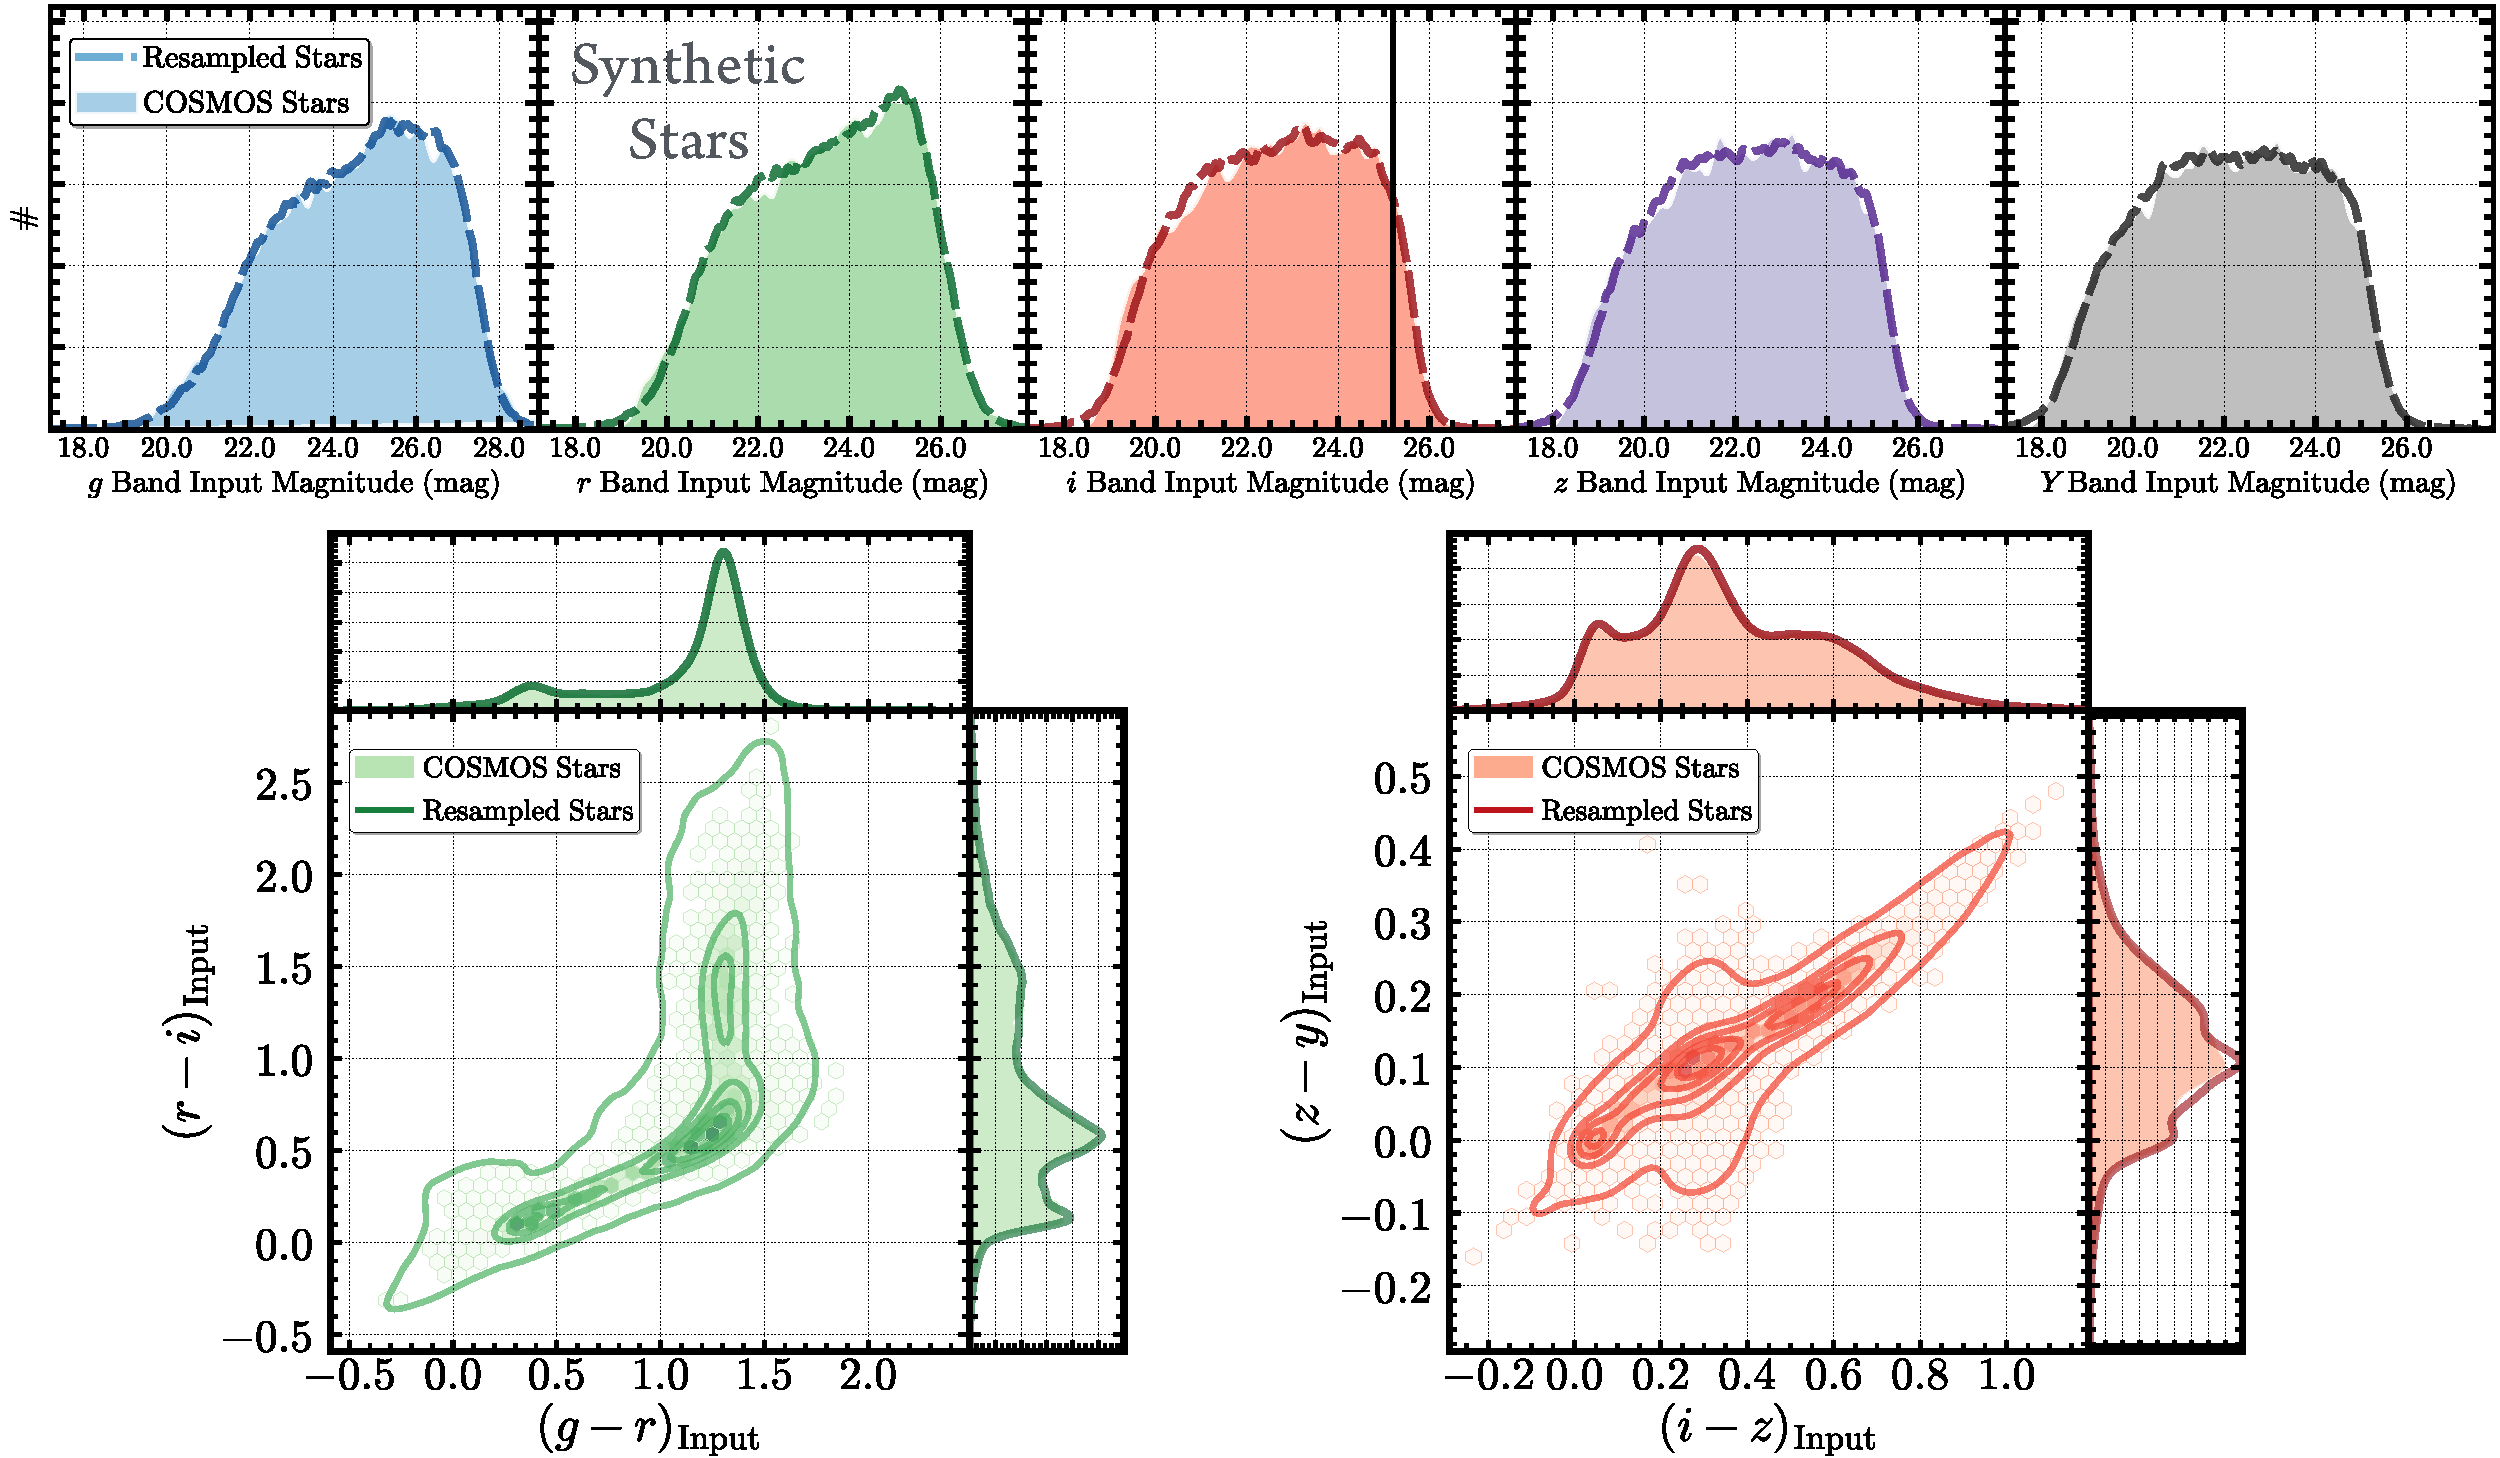
\includegraphics[width=\textwidth]{fig/synpipe_star_sample}
    \end{center}
    \caption{
        Magnitude and color distributions of the synthetic stars.
        \textbf{Upper panel} shows the 5-band magnitude distributions of the COSMOS
        stars (filled histograms) and the resampled stars (dashed lines).
        \textbf{Lower panel} shows their color-color distributions
        (left: $g-r$ v.s. $r-i$; right: $i-z$ v.s. $z-y$).
        We show the number density distribution of the COSMOS stars in hexagonal bins,
        and use contours for the resampled stars.
        }
    \label{fig:star_sample}
\end{figure*}
%% ------------------------------------------------------------------------------------ %%

%% ------------------------------------------------------------------------------------ %%
%% Fig: Galaxy Sample
\begin{figure*}
    \begin{center}
        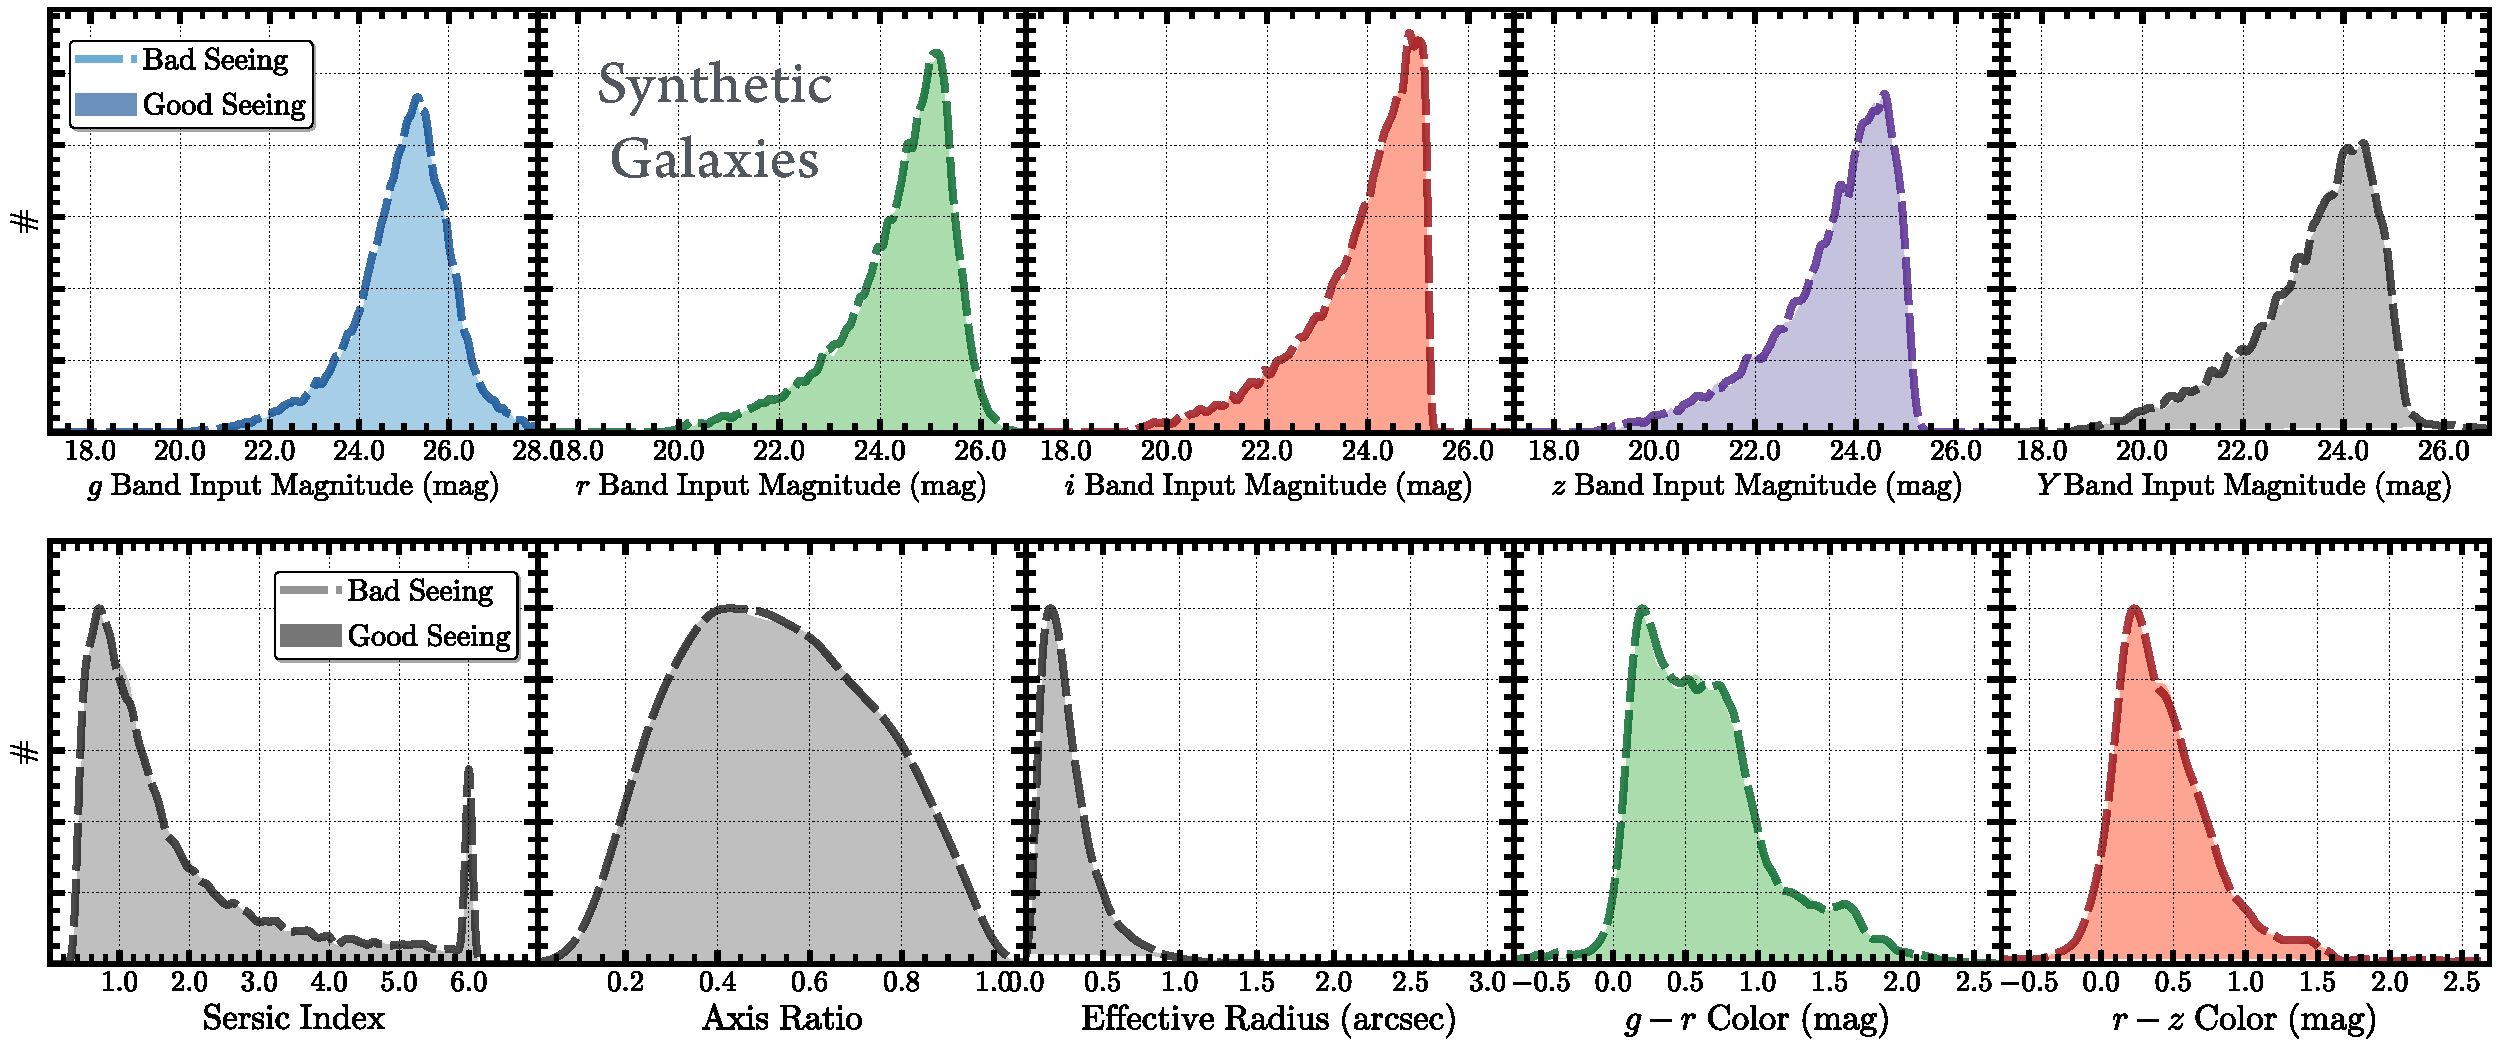
\includegraphics[width=\textwidth]{fig/synpipe_galaxy_sample}
    \end{center}
    \caption{
        Distributions of 5-band magnitudes (\textbf{upper panel}) and other properties
        (\texttt{lower panel}; from left to right are the \ser{} index, axis ratio,
        effective radius in arcsec, the $g-r$ and $r-z$ colors) of the synthetic
        galaxies.
        Objects used for the \textbf{Tract} with good seeing (filled histograms) and
        the one with bad seeing (dashed line) have almost identical distributions.
        }
    \label{fig:galaxy_sample}
\end{figure*}
%% ------------------------------------------------------------------------------------ %%

%% ------------------------------------------------------------------------------------ %%
\section{Generation of Synthetic Dataset}
    \label{sec:test}

    Here we demonstrate the application of \synpipe{} via testing the basic performance
    of HSC photometry for both stars and galaxies.

%% ------------------------------------------------------------------------------------ %%
\subsection{Test Data}

    Given the design of \synpipe{} and the data volume of HSC DR1\footnote{${\sim}70$
    TB of images}, it is not realistic to test the whole dataset.
    For this work, we select two \tracts{} in HSC Wide regions
    that fit the following criteria:

    \begin{enumerate}

        \item Not at the edge of any Wide region, so the full \tract{} is
            useful for test.

        \item Not bothered by extremely bright ($i<12$ mag), saturated star.

        \item Can represent good and bad seeing condition in the current $i$-band
            data of HSC survey.
            For the same star or galaxy, different seeing conditions affect its
            central S/N on the \texttt{coadd} images, hence it also impacts the
            detection and deblending processes in \hscpipe{}.
            Therefore, it is useful to show the photometric uncertainties under
            different seeing conditions.

    \end{enumerate}

    \noindent These regions are:
    \tract{}$=9699$ in the VVDS field (median FWHM$=0.449$\asec{} in $i$-band;
    will be referred as \texttt{goodSeeing}) and
    \tract{}$=8764$ in the XMM-LSS field (median FWHM$=0.700$\asec{};
    \texttt{badSeeing}).
    \tract{}$=9699$ also has better seeing in both $r$ and $z$-band;
    their seeing conditions in $g$ and $y$ bands are very similar.
    For both \tracts{}, the \texttt{coadd} image in each band includes data from
    20--40 \visits{}.

%% ------------------------------------------------------------------------------------ %%

%% ------------------------------------------------------------------------------------ %%
\subsection{Input Models for Stars and Galaxies}
    \label{ssec:inputs}

    In this work, we use objects from the high-resolution \hst{}/ACS observations of
    the COSMOS field to build input catalogs of realistic synthetic stars and galaxies
    with appropriate completeness for the Wide survey and reasonable five-band colors.

    For stars, we choose to use the sample from \citet{Leauthaud2007}.
    The authors select stars with clean photometry from the COSMOS images using not
    only the \texttt{SExtractor} stellar classification index (\texttt{CLASS\_STAR}),
    but also the peak surface brightness above background (\texttt{MU\_MAX}) and
    half-light radius (\texttt{RHL}).
    The classification is reliable down to $I_{\mathrm{F814W}}{\sim}25.2$ mag.
    We match this sample of stars with the HSC UltraDeep--COSMOS data that currently
    reaches to about ${\sim}27.2$ mag in $i$-band.
    After filtering the matched sample through basic quality cuts (see \ref{app:qc}),
    we gather 5-band HSC photometry for 14472 stars.
    To get a larger sample for the test, we resample the their 5-band magnitudes
    distributions using the \texttt{astroML} (\citealt{astroml}) alternative
    implementation of the \texttt{extreme-deconvolution} algorithm developed by
    \citet{Bovy2011}
    \footnote{\texttt{https://github.com/jobovy/extreme-deconvolution/}} to
    generate 100000 synthetic stars.
    In Fig \ref{fig:star_sample}, we show the magnitude and color distributions of
    the real COSMOS stars are nicely recovered by the resampled stars in all
    five-band magnitude and two color-color space.

    As for synthetic galaxies, we choose to use the single-\ser{} model of galaxies
    in the COSMOS field that have $I_{F814W} \leq 25.2$ mag.
    These models are created via method developed by \citet{Lackner2012} on the
    \textit{HST}/ACS images, and are included in \galsim{}.
    Each model is described by a total of 5 parameters: magnitude, effective radius,
    \ser{} index, axis ratio, and position angle.
    Although the single-\ser{} model is not always the best choice, its flexibility
    enables it to reasonably describe the flux distribution of most galaxies.
    Also its simplicity makes it easy to diagnose potential problems of the
    \cmodel{} photometry.
    We exclude a tiny fraction of ill-behaved models that have very high \ser{}
    index ($n_{\mathrm{Ser}} > 6.0$) or very low central surface brightness
    ($\mu_{i} < 24.0$\sb).
    We further match this COSMOS sample with the HSC UltraDeep--COSMOS data.
    after removing the objects with problematic photometry, we obtain the a sample of
    58210 synthetic galaxies with realistic 5-band HSC photometry.
    As shown in Fig \ref{fig:galaxy_sample}, the majority of these galaxies are
    faint ($i<24.0$ mag) and barely resolved ($R_{\mathrm{e}}< 1.0$\asec) galaxies.
    This sample is appropriate to test the general behaviours of photometry in
    \hscpipe{}, but is lack of relative bright galaxies ($i<20.5$ mag).

    We then create input catalogs via randomly distribute these synthetic stars and
    galaxies into the regions covered by the good and bad seeing \tracts{}.
    For stars (galaxies), we choose to use number density of 1000 (500)
    per CCD.

%% ------------------------------------------------------------------------------------ %%

%% ------------------------------------------------------------------------------------ %%

%% ------------------------------------------------------------------------------------ %%
\subsection{Running \synpipe{} Test}
    \label{ssec:running}

    We conduct these tests on the cluster (\texttt{Master}) at Kavli-IPMU using
    the HSC DR1 data stored there.
    The \texttt{addFakes.py} step takes ${\sim}1.5$ hours per \tract{} in each
    band; same process takes longer for the test of galaxies (${\sim}3.0$ hours per
    \tract{} in each band) as the \galsim{} simulation is more time consuming.
    The \texttt{stack.py} and \texttt{multiBand.py} together take ${\sim}3.5$ hours
    per \tract{}.

    We match the results with the input catalogs using a 2 pixels matching radius
    to generate output catalogs for \forced{} and \unforced{} photometry
    in each band.
    We also match the input catalogs with the original HSC catalogs to identify the
    ``ambiguously blended'' objects that are right on top of the flux peak of a real
    object.
    These objects are useful in the WL-related statistical tests (see Murata et al.
    in prep. for more details), but will not help test photometry, hence they will
    be excluded later

    The detailed log of the entire tests can be found here:
    \url{goo.gl/VINOVP}.
    User should be able to reproduce the results presented in this work using this
    information.
    It can also serve as a brief manual for running \synpipe{} test.

%% ------------------------------------------------------------------------------------ %%

%% ------------------------------------------------------------------------------------ %%
\section{Results on Photometric Performance}
    \label{sec:result}

    Here we show the general performance of \hscpipe{} for stars (galaxies)
    mainly through the \forced{} PSF (\cmodel{}) photometry.
    Although \hscpipe{} provides more options (e.g. aperture and Kron photometry),
    these two are the most appropriate and relevant ones for magnitude and colors of
    star and galaxy as they consider the effects of PSF in different bands,
    and are consistent across all bands in terms of position and shape.

%% ------------------------------------------------------------------------------------ %%

%% ------------------------------------------------------------------------------------ %%
%% Fig: Magnitude v.s S/N for stars
\begin{figure*}
    \begin{center}
        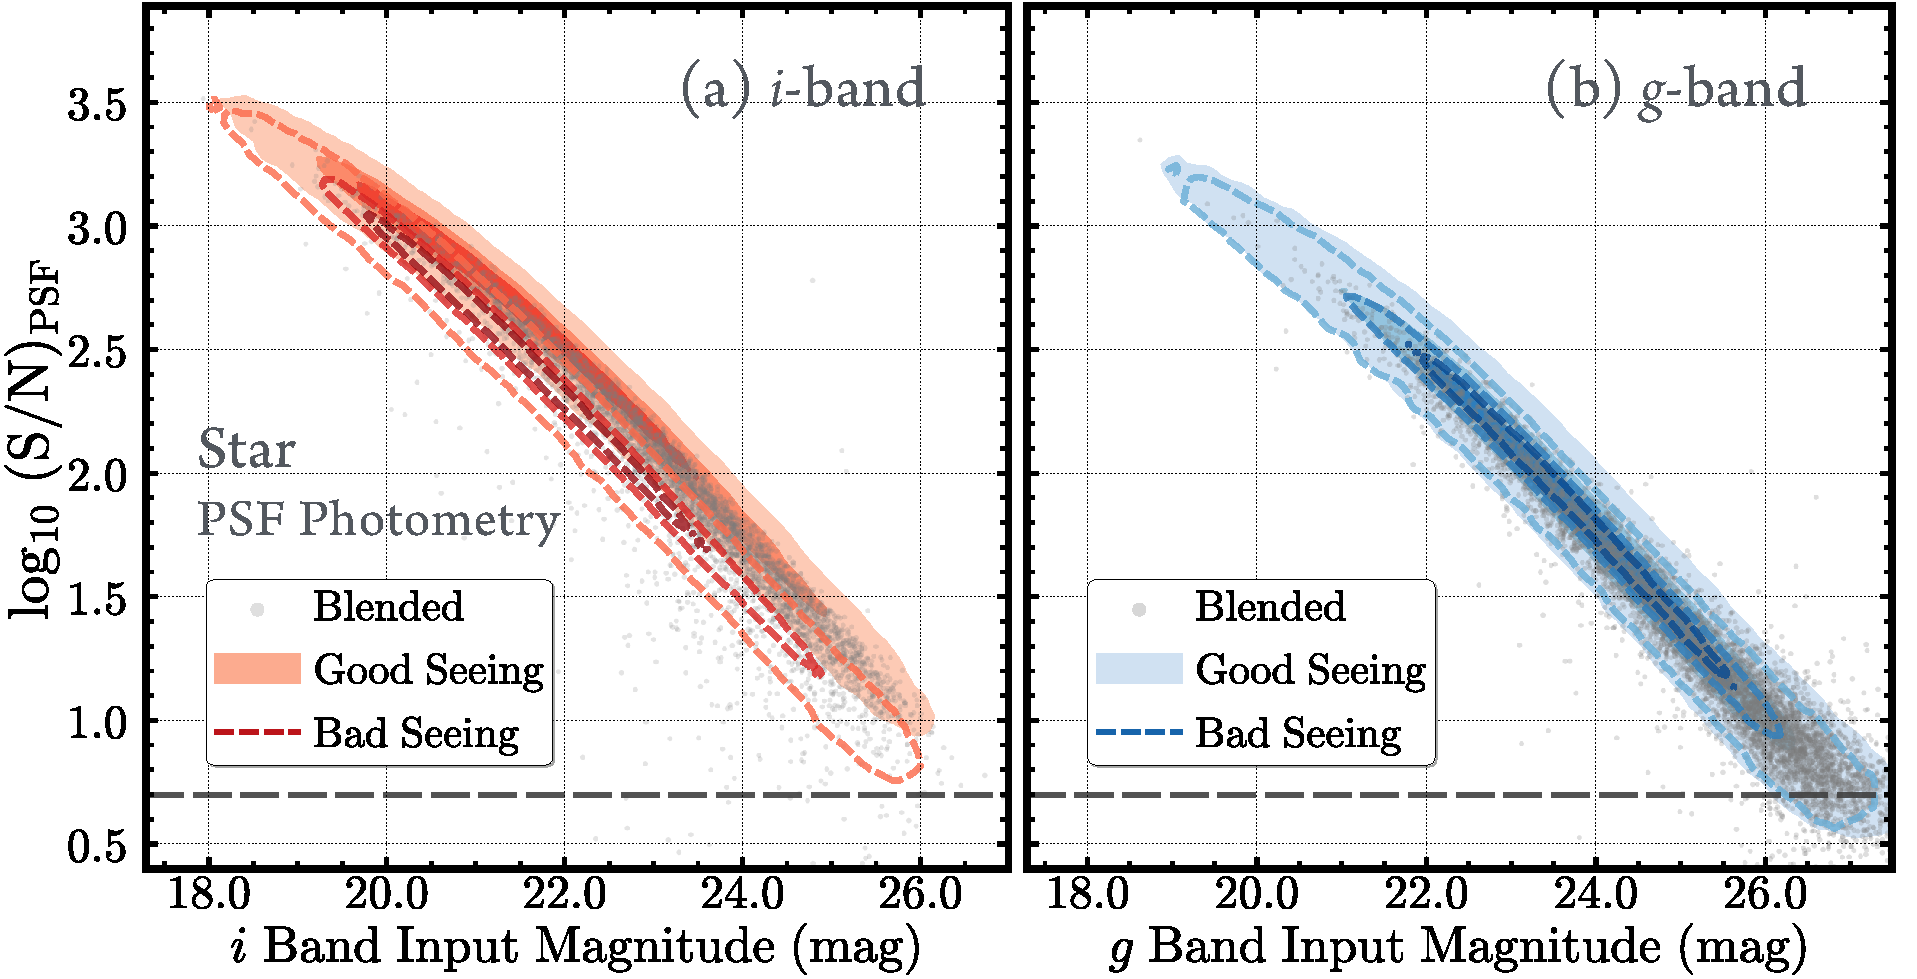
\includegraphics[width=\textwidth]{fig/synpipe_psf_sn}
    \end{center}
    \caption{
        Relations between input magnitudes (\textbf{left}: $i$-band; \textbf{right}:
        $g$-band) of synthetic stars and the $log(S/N)$ measured by \hscpipe{} PSF
        photometry.
        Hexagonal binned density plots and contours show the distributions for
        stars in the \tract{} with good and bad seeing.
        The highly blended stars are highlighted using scatter plots.
        A grey dashed line marks $S/N = 5$.
        }
    \label{fig:star_sn}
\end{figure*}
%% ------------------------------------------------------------------------------------ %%

%% ------------------------------------------------------------------------------------ %%
%% Fig: Accuracy of Forced PSF Magnitudes
\begin{figure*}
    \begin{center}
        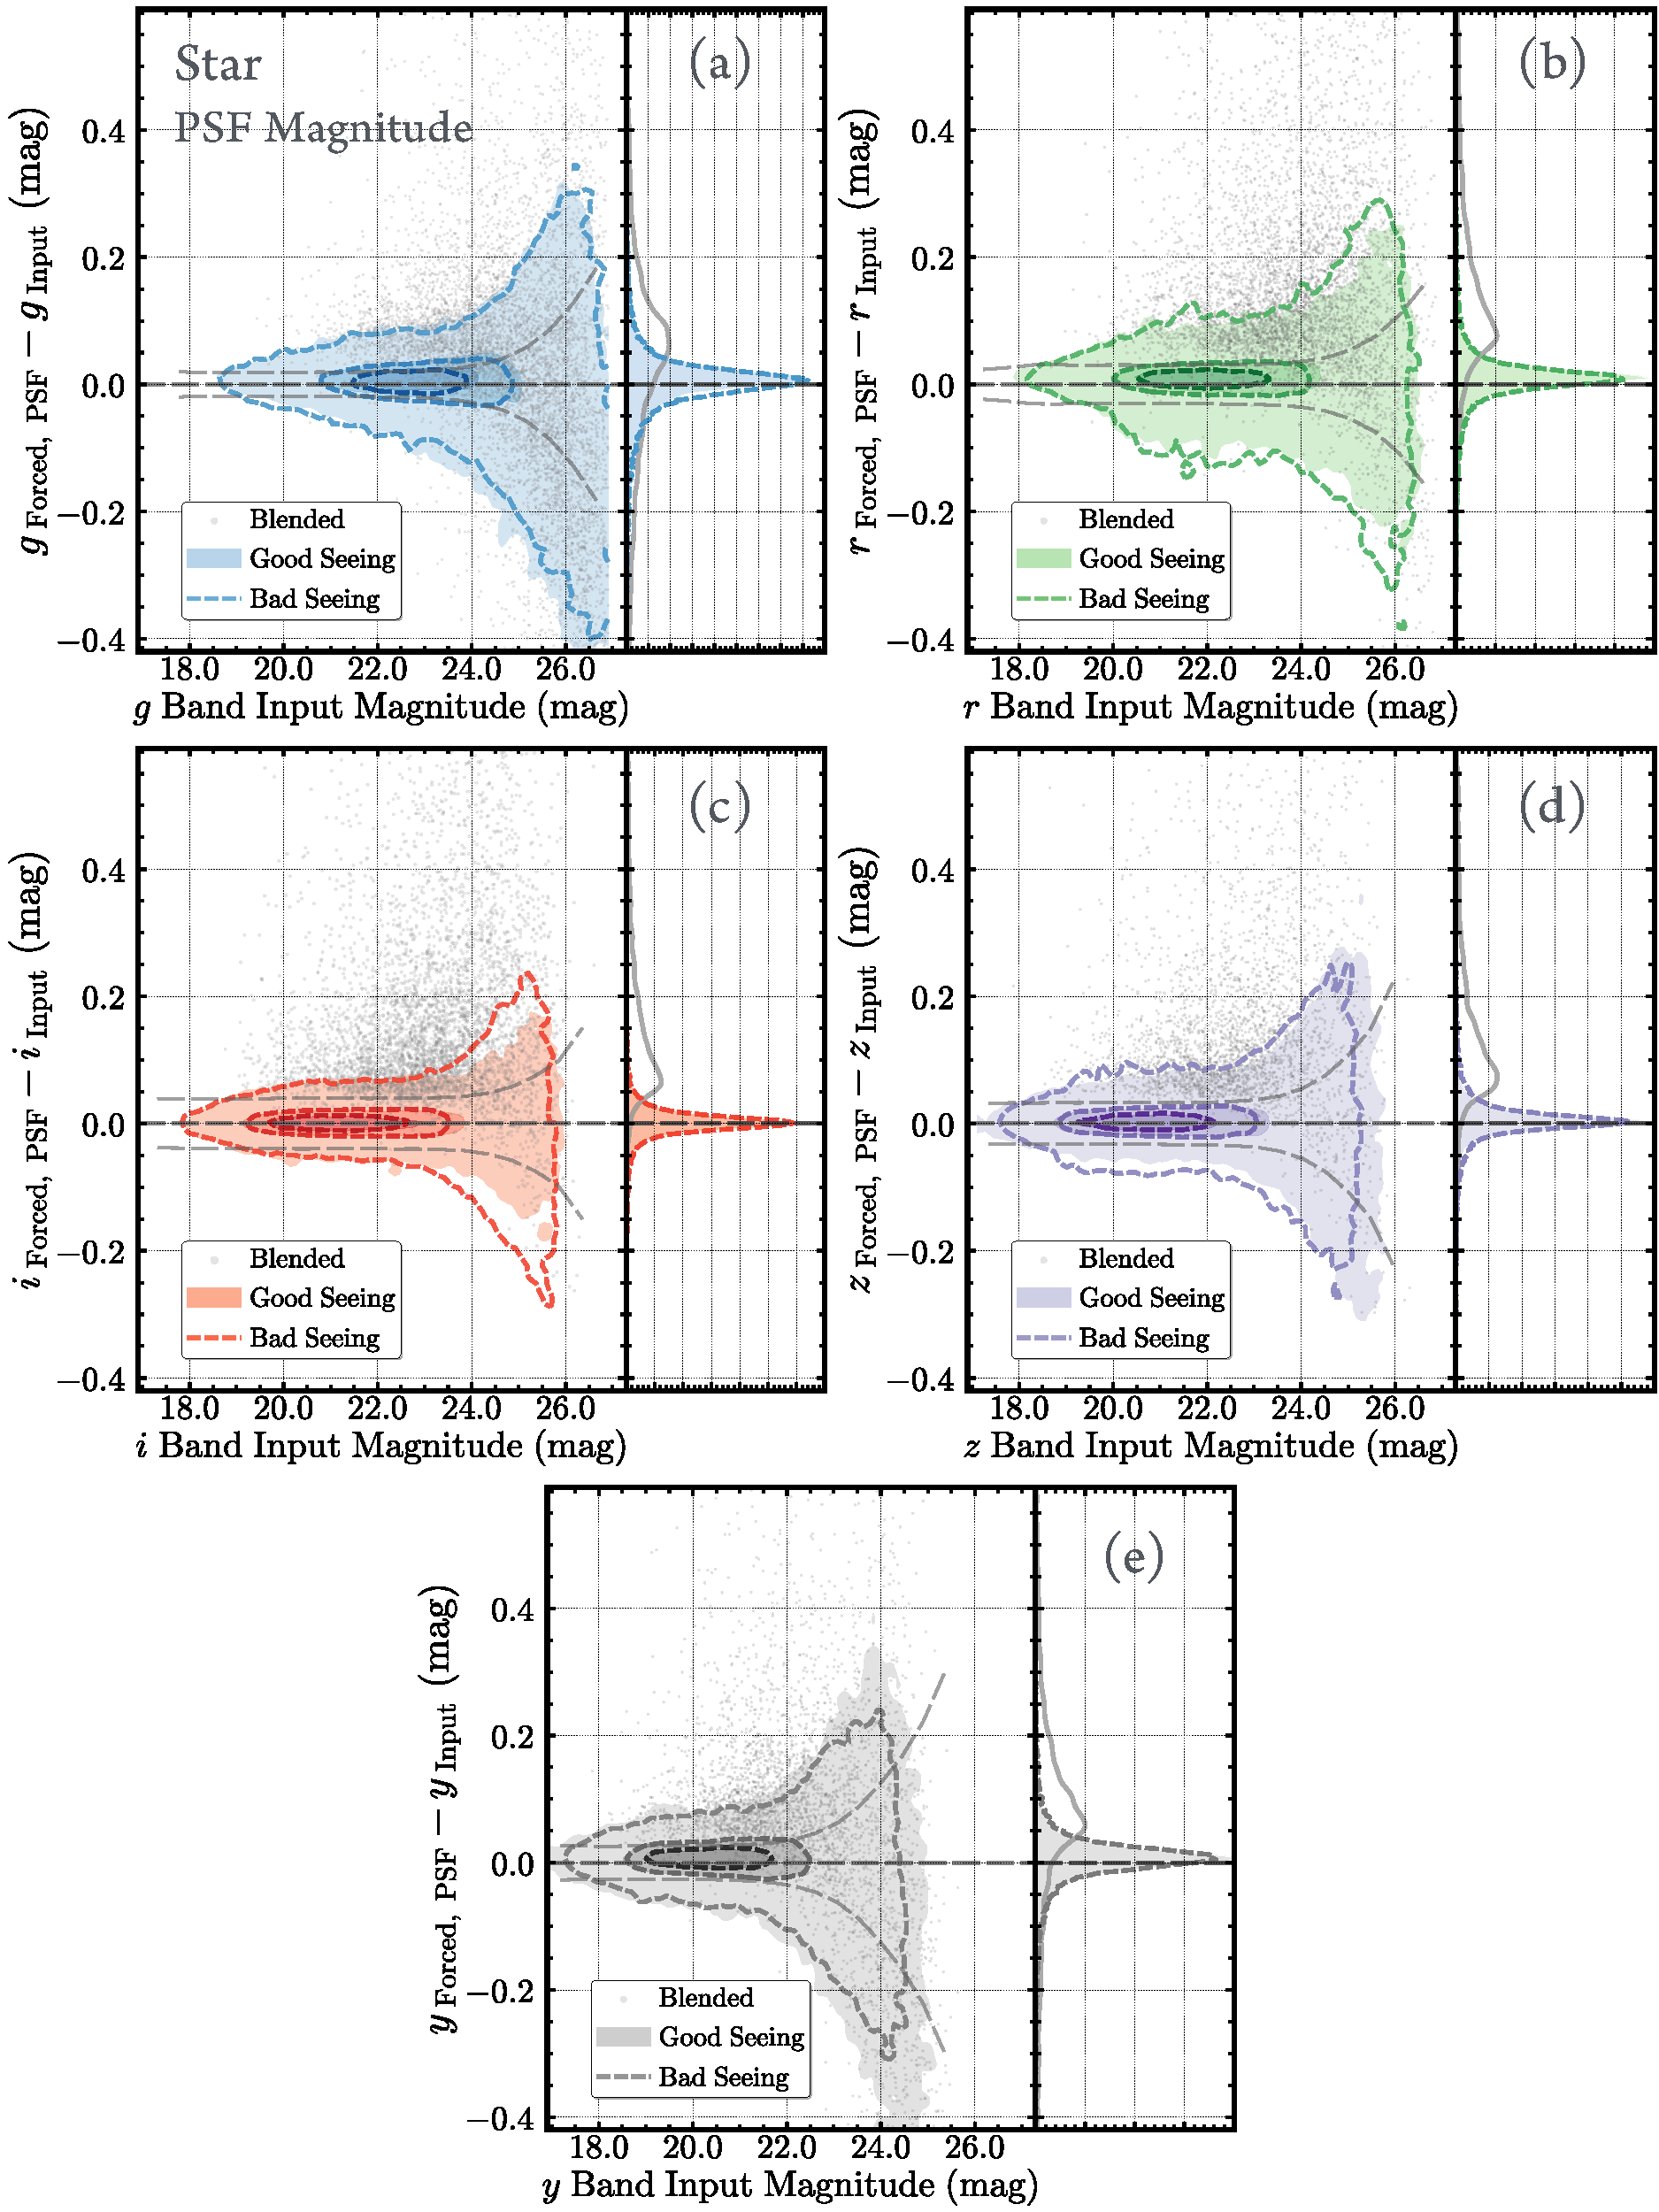
\includegraphics[width=16cm]{fig/synpipe_psf_mag}
    \end{center}
    \caption{
        Accuracies of the \texttt{hscpipe} PSF photometry for synthetic stars measured
        by the difference between input and output \forced{} PSF magnitudes.
        Plot [a, b, c, d, e] shows the results for [$g$, $r$, $i$, $z$, $y$]-band.
        In each plot, left panel shows the relation between input magnitude and
        magnitude difference.
        Hexagonal binned density plot and contour are for the synthetic galaxies from
        good and bad seeing \tracts{}.
        Highly blended objects are highlighted using scattered plot.
        The long-dashed line marks zero magnitude difference, while the pair of
        dashed lines outline the running-median of PSF magnitude errors
        (including the uncertainties in aperture correction).
        Right panel shows the distributions of the magnitude differences for objects
        in good (filled) and bad (solid line) seeing \tracts{}.
        The dashed line is for the distribution of highly blended objects.
        }
    \label{fig:psf_mag}
\end{figure*}
%% ------------------------------------------------------------------------------------ %%

%% ------------------------------------------------------------------------------------ %%
%% Fig: Difference between the Unforced and Forced Magnitudes
\begin{figure*}
    \begin{center}
        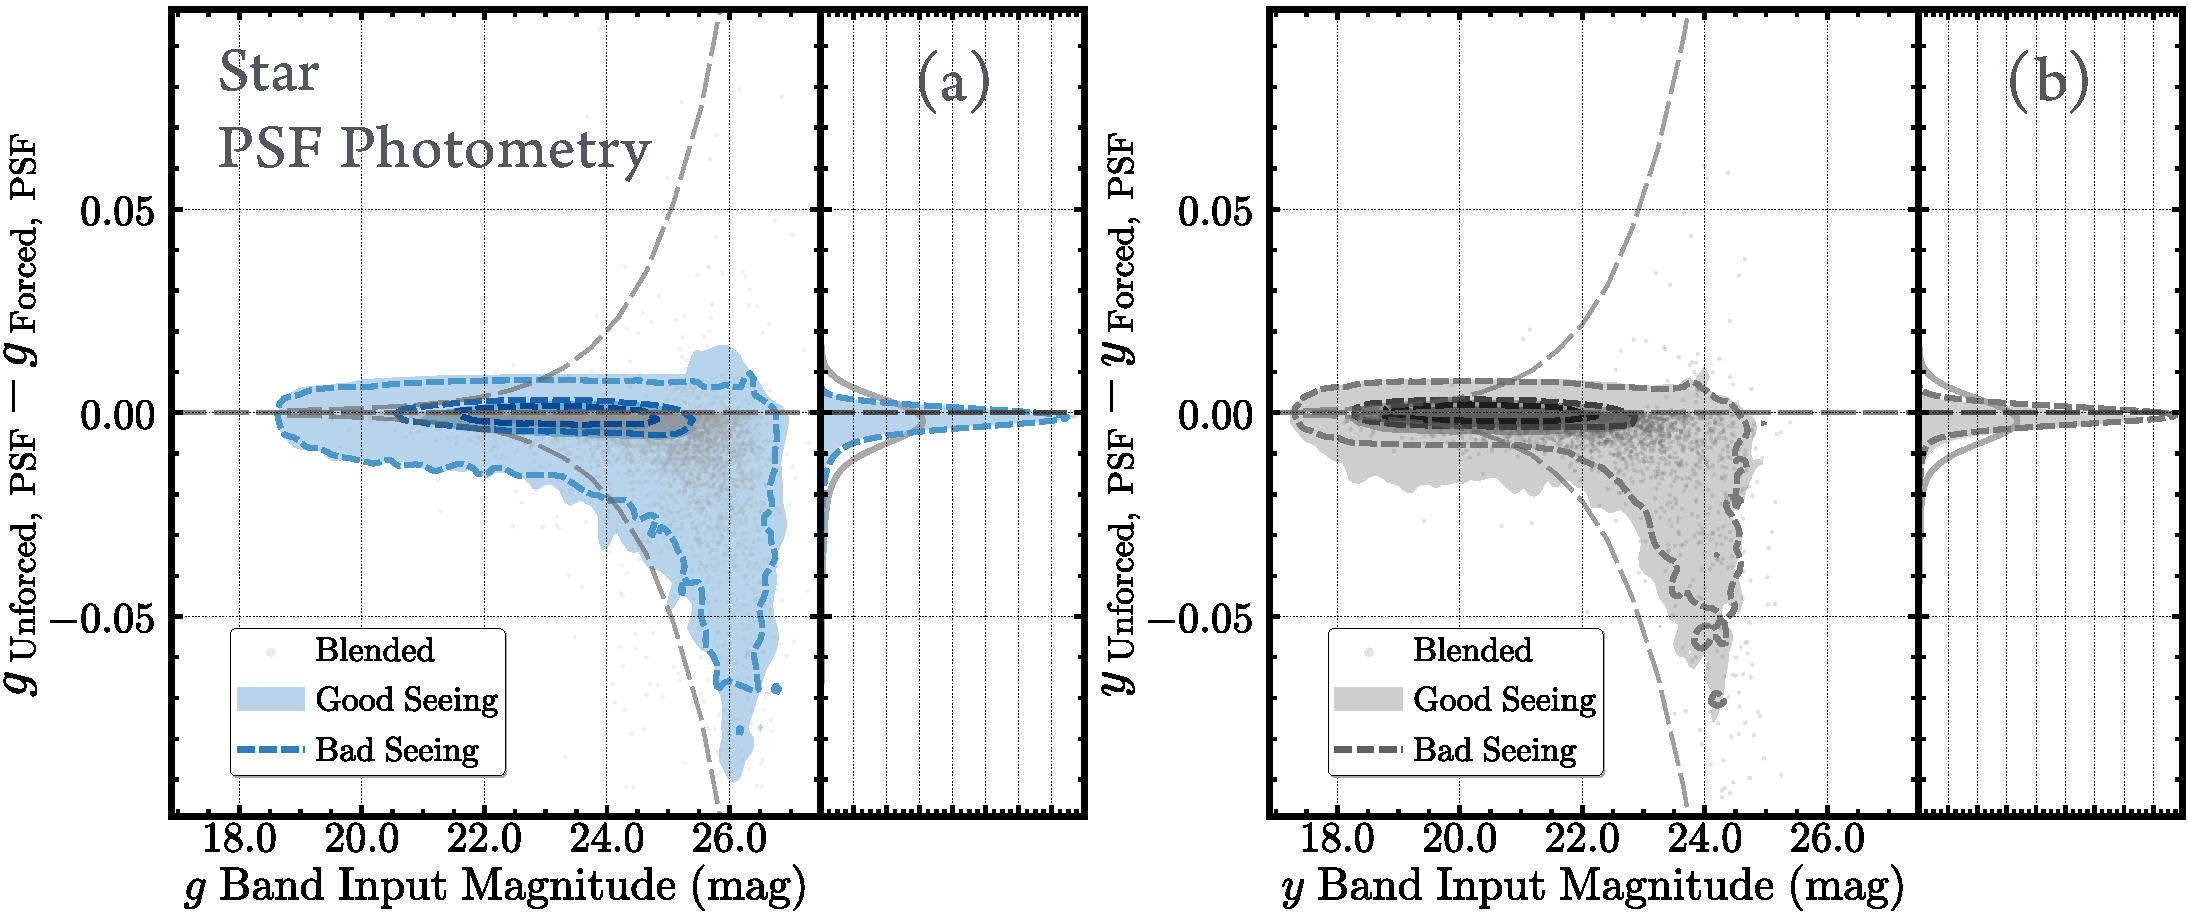
\includegraphics[width=\textwidth]{fig/synpipe_psf_diff}
    \end{center}
    \caption{
        The magnitude differences between the \unforced{} and \forced{}
        PSF photometry for synthetic stars in $g$- (\textbf{left} and $y$-band
        (\textbf{right}).
        Other formats are identical to the plots in Fig \ref{fig:psf_mag}.
        }
    \label{fig:psf_diff}
\end{figure*}
%% ------------------------------------------------------------------------------------ %%

%% ------------------------------------------------------------------------------------ %%
%% Fig: Accuracies of the PSF color
\begin{figure*}
    \begin{center}
        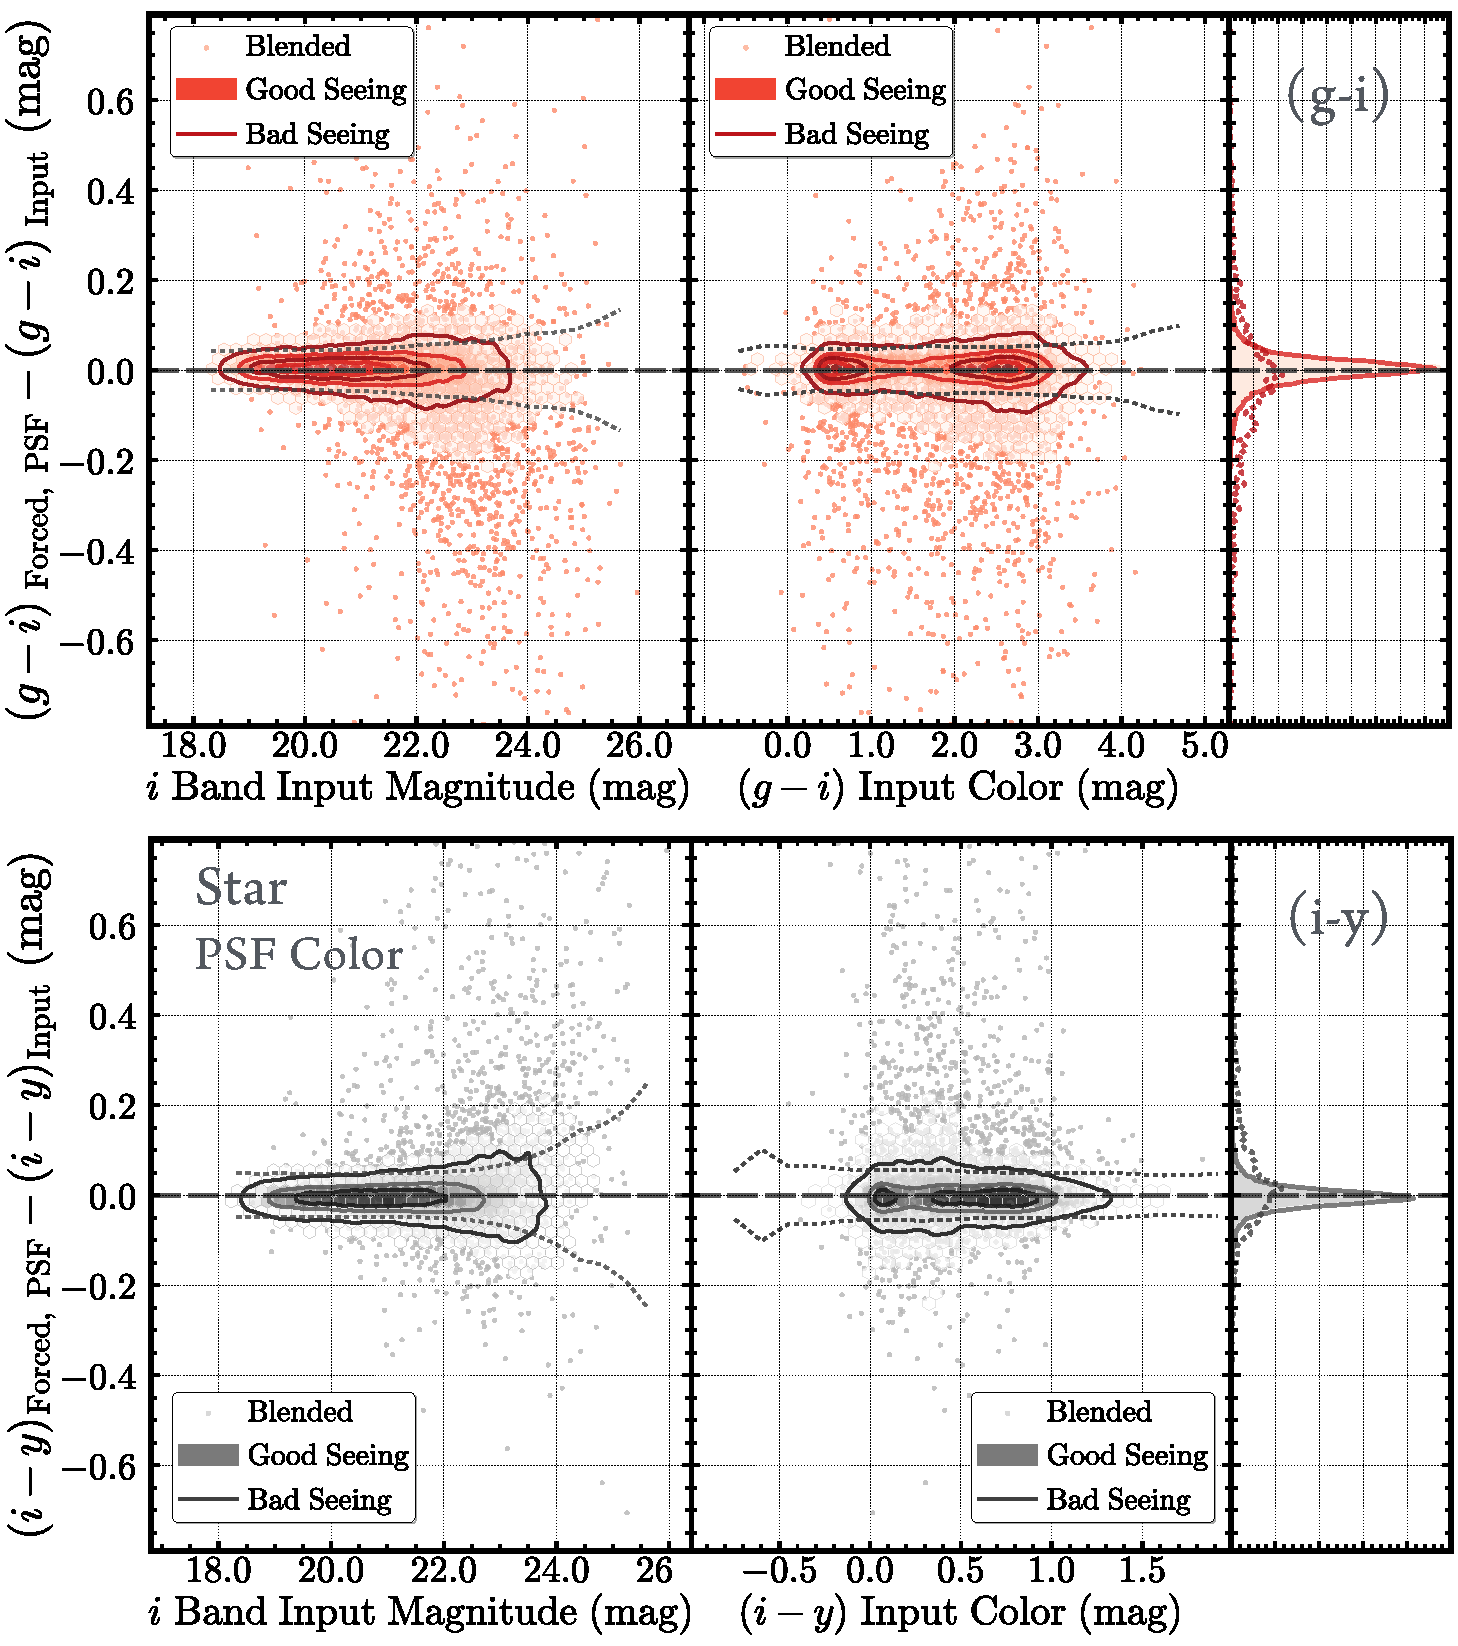
\includegraphics[width=\textwidth]{fig/synpipe_psf_color}
    \end{center}
    \caption{
        Accuracies of the color measurements for synthetic stars via the differences
        between input and \forced{} PSF colors.
        The \textbf{Upper panels} and \textbf{lower panels} are for $g-i$ and $i-y$
        colors separately.
        The \textbf{left} column shows the relation between input magnitude and
        the color difference, and the \textbf{right} one uses the input colors as
        x--axis instead.
        Other formats are identical to the plot in Fig \ref{fig:psf_mag}.
        }
    \label{fig:psf_color}
\end{figure*}
%% ------------------------------------------------------------------------------------ %%

%% ------------------------------------------------------------------------------------ %%
%% Fig: Color-Color Distributions of the Input and Measurements for stars
\begin{figure*}
    \begin{center}
        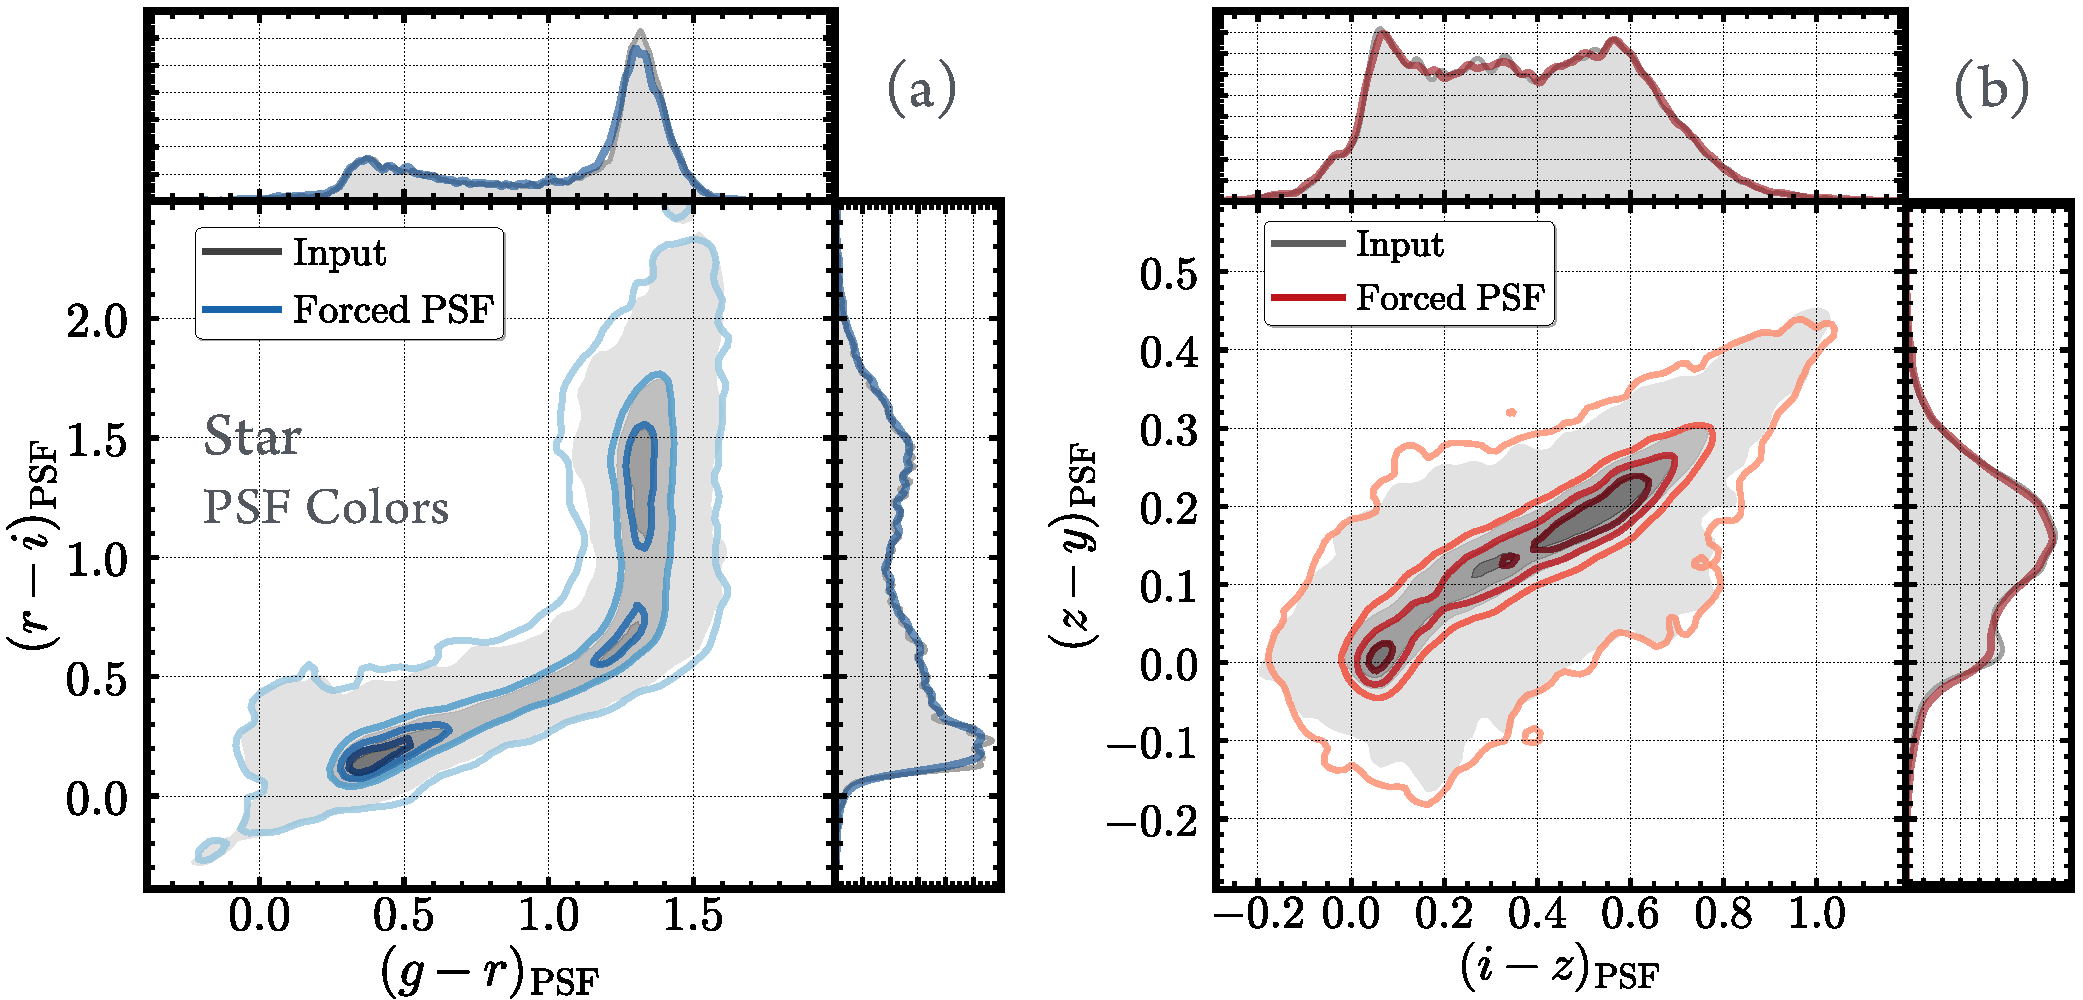
\includegraphics[width=\textwidth]{fig/synpipe_psf_cdist}
    \end{center}
    \caption{
        Evaluations of the accuracy of color measurements for synthetic stars using
        the color-color distributions.
        \textbf{Left} uses $(g-r)$ v.s. $(r-i)$ colors, and the \textbf{right} one
        uses $(i-z)$ and $(z-y)$ colors.
        The filled contours and shaded histograms reflect the distributions for input
        colors.
        The empty contours and solid-line histograms show the distributions recovered
        by \hscpipe{}.
        }
    \label{fig:psf_cdist}
\end{figure*}
%% ------------------------------------------------------------------------------------ %%

%% ------------------------------------------------------------------------------------ %%
\subsection{PSF photometry of Stars}
    \label{ssec:psf}

    In \hscpipe{}, the PSF magnitude is derived using matched-filter method that
    depends on the best-fit PSF model and uses the Lanczos interpolation to shift
    PSF model.
    The error of PSF magnitude from \hscpipe{} only considers the per-pixel noise,
    not the uncertainty of the centroid.
    \hscpipe{} also estimates aperture correction for PSF photometry.
    For more details please see Section 4.9.5 of Bosch\etal (in prep.).

    In our tests, we randomly inject ${\sim}100000$ stars to each \tract{} in all
    five-bands.
    Among these stars, ${\sim}3$--$4$\% of them locate within 2 pixels to the centroids
    of real objects.
    We remove them from the sample to avoid confusion in the comparisons.
    After this step, there are still ${\sim}1$--$3$\% of the remaining synthetic stars
    have no match in the \synpipe{} outputs.
    They could be either below the detection threshold or ambiguously blended with real
    objects.
    The input $i$-band magnitudes of these unmatched stars are on average ${\sim}0.9$
    mag fainter than the matched ones.
    The fraction of unmatched stars is slightly higher in the bad seeing \tract{},
    which is consistent with the expectation of seeing-dependent limit magnitude,
    although the difference in not very significant.
    For the matched stars, we select the primary detections
    (\texttt{detect.is-primary=True}) that have good photometric quality
    (see Appendix \ref{app:qc} for details).
    This gives us ${\sim}83000$ stars in each \tract{}.

    Next, we isolate the stars that are misidentified by \hscpipe{} as extended
    objects using the \texttt{classification.extendedness} parameter in each band.
    The fraction of misclassification is ${\sim}8$--$15$\%, and clearly depends on
    seeing conditions.
    For the same reason, $g$-band has the highest fraction of misclassification,
    while $i$-band is recommended for selecting point sources.
    The misclassified stars are on average ${\sim}1$ mag fainter than the others.
    We exclude them from the photometric comparison below, and will further discuss
    the star--galaxy separation issue in Section \ref{ssec:sg}.

    In the following comparisons, we will always show the results from the
    \textbf{good seeing} and \textbf{bad seeing} \tracts{} separately, because it
    is important to understand the impact of seeing on photometric accuracies,
    and to test whether \hscpipe{} can deliver unbiased photometry under different
    seeing conditions.

    Besides seeing, ``blendedness'' ($b$; parameter that describes on what level
    the flux distribution of one object is affected by others; please see
    Appendix \ref{app:defineb} for precise definition, and see Murata\etal in prep.
    for details) is another factor that influences the photometric accuracy.
    We therefore separate the samples into relative isolated and highly blended
    groups based on the $b$ values.
    Assuming zero pixel noise, $b$ of object $A$ reflects the fraction of flux
    within the \texttt{Footprint} of $A$ that comes from other objects.
    Ideally, $b=0$ means perfect isolation, and $b{\sim}1$ means completely
    confused with other object.
    Here we use $b>0.05$ to define blended stars (${\sim}4$--$9$\%).
    Fraction of highly blended stars slightly increases in the bad seeing \tract{}.
    We highlight these stars separately as well, and will discuss more about the
    impact of blendedness in Section \ref{ssec:blendedness}.

\subsubsection{Input magnitude and the \s2n{} of PSF photometry}

    We first briefly discuss the relationship between input magnitude and the
    signal-to-noise ratio of the output PSF photometry.
    Here, we simply define the \s2n{} as
    $\mathrm{Flux}_{\mathrm{PSF}}/\mathrm{Flux\_Err}_{\mathrm{PSF}}$ in each band
    without considering the aperture correction.
    This will help us visualize
    1) the detection limit for point sources,
    2) the impact of seeing condition on PSF photometric,
    3) and the scatter of photometric accuracies at fixed input magnitude given all
       the realistic features of HSC images (e.g. background subtraction, nearby
       object, optical artefacts).
    We show the results for $g$- and $i$-band in Fig \ref{fig:star_sn}, and find tight
    relations in both bands.

    As expected, we clearly see that the seeing condition impacts the \s2n{} of point
    sources at fixed input magnitude.
    In $i$-band, the \tract{} with slightly worse seeing (0.7\asec{}) shows systematically
    lower \s2n{} comparing to the one with better seeing (0.5\asec{}).
    As for the $g$-band, since the two \tracts{} share similar seeings now, they also
    follow similar relations.
    We also see that the blendedness can also affect accuracies of PSF photometry.
    In $i$-band, the highly blended synthetic stars scatter toward lower \s2n{} at
    fixed magnitude.
    Interestingly, the effect is not obvious in $g$-band, suggesting the deblending
    process and photometric quality of blended objects also depend on seeing condition.

    At \s2n{}$=5$, HSC Wide can detect stars as faint as ${\sim}26.5$ mag in both $g$ and
    $i$-band at average seeing condition, which is consistent with the values found
    in \citet{HSCDR1}.
    At the same time, it is worth reminding the users of HSC data that the detection
    limit will show spatial variations due to the seeing conditions.

\subsubsection{Accuracy of PSF magnitude}

    Now, we will look into the accuracies of PSF magnitudes in all five bands
    independently.
    In Fig \ref{fig:psf_mag}, we show the relations between the input magnitude and the
    magnitude difference from the \hscpipe{} \forced{} PSF photometry.

    The overall performance of PSF photometry is excellent.
    In $i$-band, the median magnitude difference for \tract{} with 0.45\asec{} seeing is
    around ${\sim}0.015$ mag (${\sim}1.5$\% accuracy) at
    $i_{\mathrm{Input}}{\sim}19.0$ mag.
    At $i_{\mathrm{Input}}{\sim}24.0$ mag, the average accuracy of PSF
    magnitude keeps at ${\sim}3$\% level (${\sim}0.036$ mag average difference).
    Down to $i_{\mathrm{Input}}{\sim}25.2$ mag, the average accuracy decreases to
    ${\sim}7$\% level with an average ${\sim}0.072$ mag difference.
    The \tract{} with worse seeing shows similar accuracy of PSF photometry at
    $i_{\mathrm{Input}}<23.5$ mag.
    At faint end, the accuracy becomes slightly worse: ${\sim}5$\% accuracy around
    $i_{\mathrm{Input}}{\sim}24.0$ mag; and ${\sim}11$\% accuracy around
    $i_{\mathrm{Input}}{\sim}25.2$ mag.
    \citet{HSCDR1} evaluates the accuracy of PSF photometry via external comparisons
    with the PS1 PV2 and SDSS data at $i<21$ mag, and finds a 1-2\% level accuracy,
    which is consistent with our results.
    At fainter magnitude, external comparisons become difficult due to the lack of deep
    imaging data at HSC level and the impact of the color-term when comparing photometry
    using different filters.
    The results from \synpipe{} hence provide more useful evaluations down to the
    detection limit\footnote{Strictly speaking, the uncertainties here should be
    considered as lower limit as the \synpipe{} now does not consider the uncertainties
    in PSF modeling.}.

    We also see that the accuracy of PSF photometry does not strongly depend on filters.
    The forced PSF magnitude in $r$ and $z$-band have very similar accuracy with
    $i$-band (1.5-4.0\% at $19.0 < r_{\mathrm{Input}} < 24.0$ mag, ${\sim}8$\% down to
    $r_{\mathrm{Input}}{\sim}25.2$ mag;
    1.0-5.0\% at $19.0 < z_{\mathrm{Input}} < 24.0$ mag, ${\sim}10$\% down to
    $z_{\mathrm{Input}}{\sim}25.2$ mag).
    The accuracies in $g$- and $y$-band become slightly worse (
    1.5-7.0\% at $19.0 < g_{\mathrm{Input}} < 24.0$ mag, ${\sim}13$\% down to
    $g_{\mathrm{Input}}{\sim}25.2$ mag;
    1.5-5.0\% at $19.0 < y_{\mathrm{Input}} < 23.0$ mag, ${\sim}12$\% down to
    $y_{\mathrm{Input}}{\sim}24.0$ mag;), but the differences can be attributed to the
    differences in seeing conditions.

    For relative isolated stars, \hscpipe{} provides unbiased PSF photometry down to
    very faint magnitude in $i$- and $z$-band.
    For $g$-, $r$-, and $y$-band, we find small offsets in the distributions of magnitude
    differences, which indicates \hscpipe{} tends to underestimate the fluxes of stars
    in these bands by ${\sim}0.01-0.02$ mag.
    Although the exact cause of this offset is unclear (could still be related to
    differences in seeing), it will not affect the accuracies of magnitudes of colors.

    At the same time, the story for highly blended stars is very different.
    \hscpipe{} on average systematically underestimates the total fluxes of them by
    $0.05$--$0.10$ mag at fixed input magnitude.
    We see the same effect in all bands, and the impact of blendedness becomes
    increasingly significant at fainter magnitude.
    It is therefore important to keep this in mind when using PSF photometry for point
    sources in HSC data.

    We also test the \unforced{} PSF photometry in all five bands, and find very similar
    accuracies.
    During the measurement of \forced{} PSF photometry, \hscpipe{} fixes the centroid
    of the PSF model across all five band.
    Therefore, the magnitude difference between \forced{} and \unforced{} PSF magnitudes
    indicates the photometric uncertainties induced by differences in the accuracies of
    astrometric calibrations and PSF modeling among different bands.
    We highlight the differences between \forced{} and \unforced{} PSF photometry of
    $g$- and $y$-band in Fig \ref{fig:psf_diff}.
    The overall difference is very small ($<0.01$ mag), but it also suggest that
    \hscpipe{} \unforced{} PSF photometry systematically recovers slightly more fluxes
    at very faint end.

\subsubsection{Accuracy of the PSF colors}

    Color measurement based on PSF photometry is the most appropriate one for point
    sources, and is therefore important to many scientific goals of the HSC survey
    (e.g. study of the Milky Way structure, selection of unique stellar objects or
    high-redshift quasars, and the accurate star--galaxy separation).

    In Fig \ref{fig:psf_color}, we evaluate the accuracies of the \forced{} $(g-i)$
    and $(i-y)$ PSF colors via comparing the error in color measurements with both
    input magnitudes and input colors.
    These results suggest that \hscpipe{} provides accurate and unbiased PSF color
    estimates for synthetic stars with realistic color distributions down to very faint
    magnitude.
    For $(g-i)$ color, the average uncertainty around $i_{\mathrm{Input}}{\sim}19.0$ mag
    is ${\sim}0.025$ mag, and increases to ${\sim}0.11$ mag at
    $i_{\mathrm{Input}}{\sim}24.0$ mag.
    The results are very similar for the $(i-y)$ color.
    We also find that the accuracies of PSF colors do not depend on the input colors of
    the synthetic stars or the seeing conditions.
    For instance, the accuracy of $(g-i)$ color for \tract{} with bad seeing only becomes
    slightly worse in the very faint end (${\sim}0.14$ mag at
    $i_{\mathrm{Input}}{\sim}24.0$ mag) comparing to the results for good seeing \tract{}.

    We further illustrate the accuracies of PSF colors via comparing the distributions
    of colors for the input synthetic stars and the ones recovered by \hscpipe{}
    (see Fig \ref{fig:psf_cdist}).
    Using four different colors and two color--color planes, we show that the \forced{}
    PSF colors can accurately reproduce the distributions of all four colors and the
    2-D color-color distributions.

    As for the highly blended stars, on Fig \ref{fig:psf_color}, we see that on average
    they still have larger uncertainties in colors comparing to the relative isolated
    ones.
    For $(g-i)$ color, the average color uncertainty is ${\sim}0.1$ mag larger for the
    highly blended stars at fixed input magnitude.
    However, the biases in color measurements for these stars are less severe than
    the magnitude measurements.
    Although the blended stars still show slightly bluer (redder) $(g-i)$ ($(i-y)$)
    colors comparing to the isolated ones and the input values, the differences in the
    distributions of color uncertainties of blended and isolated stars are less striking
    than the ones for magnitude differences.

%% ------------------------------------------------------------------------------------ %%

%% ------------------------------------------------------------------------------------ %%
%% Fig: Magnitude v.s S/N for galaxies
\begin{figure*}
    \begin{center}
        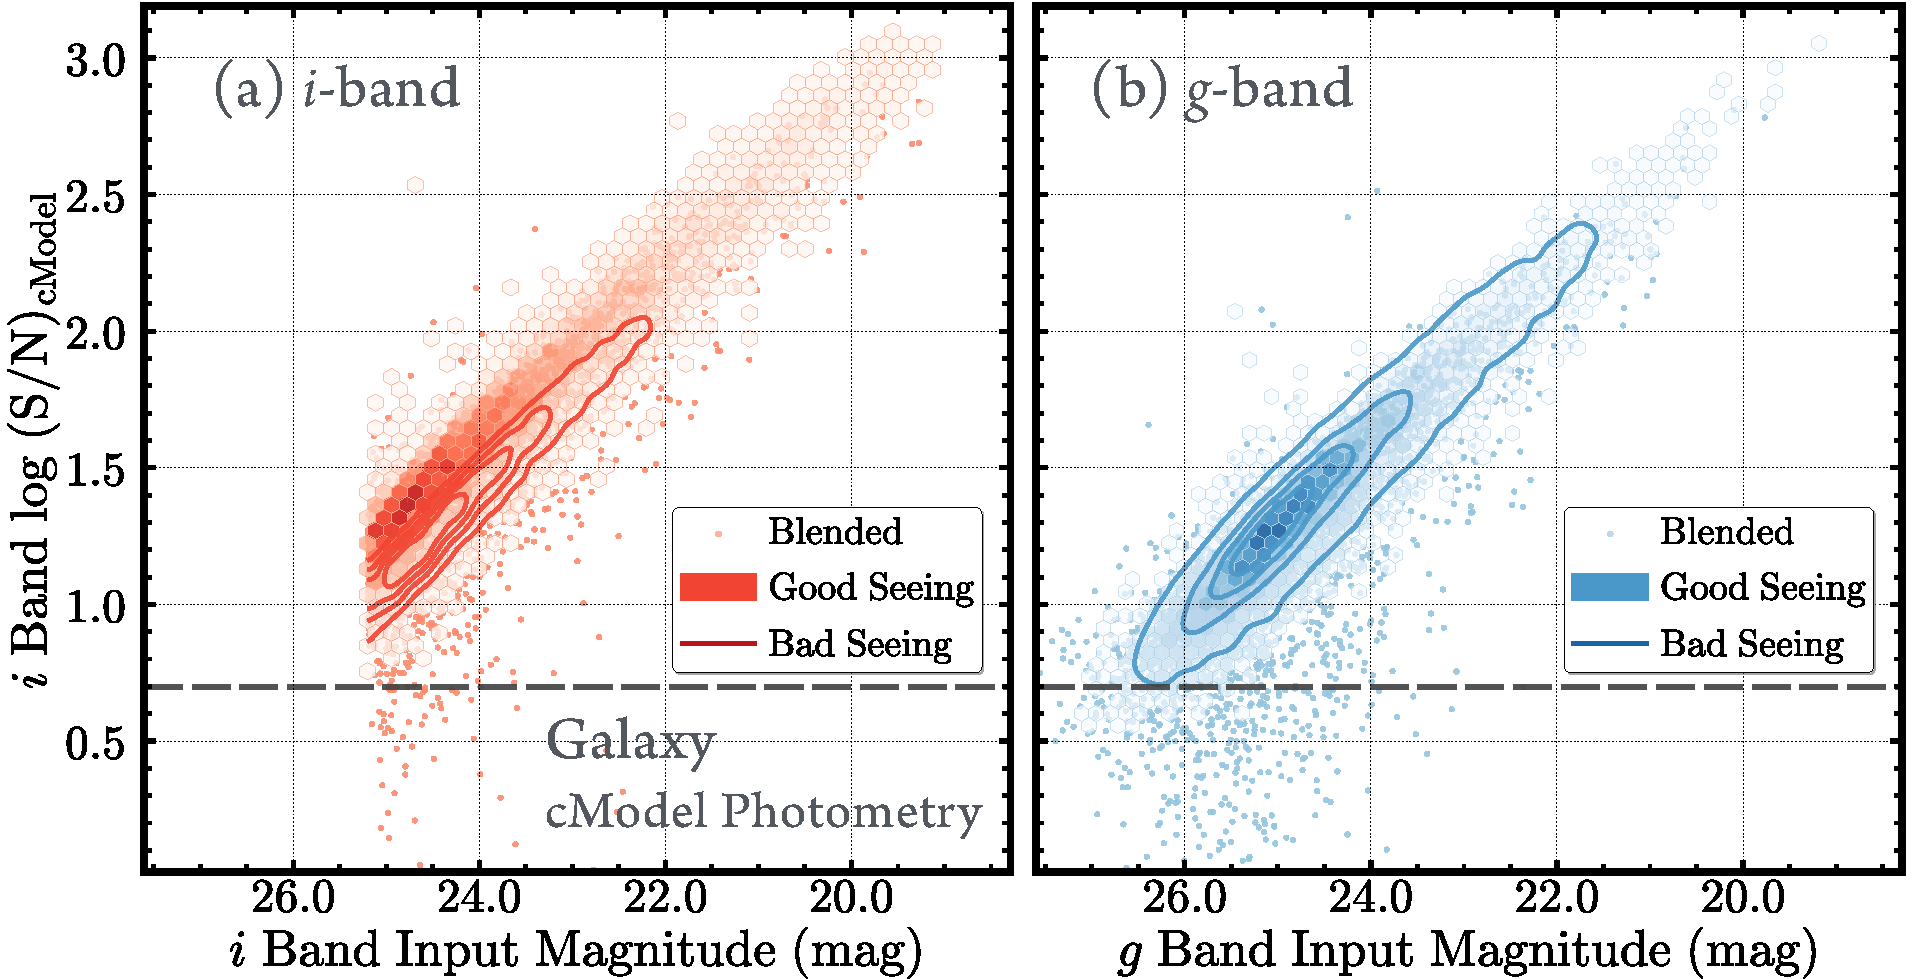
\includegraphics[width=\textwidth]{fig/synpipe_galaxy_sn}
    \end{center}
    \caption{
        Relations between input magnitudes (\textbf{left}: $i$-band; \textbf{right}:
        $g$-band) of synthetic galaxies and the $log(S/N)$ measured by \hscpipe{}
        \cmodel{} photometry.
        Other formats are very similar to Fig \ref{fig:star_sn}
        }
    \label{fig:cmodel_sn}
\end{figure*}
%% ------------------------------------------------------------------------------------ %%

%% ------------------------------------------------------------------------------------ %%
%% Fig: Accuracy of Forced cModel Magnitudes for galaxies
\begin{figure*}
    \begin{center}
        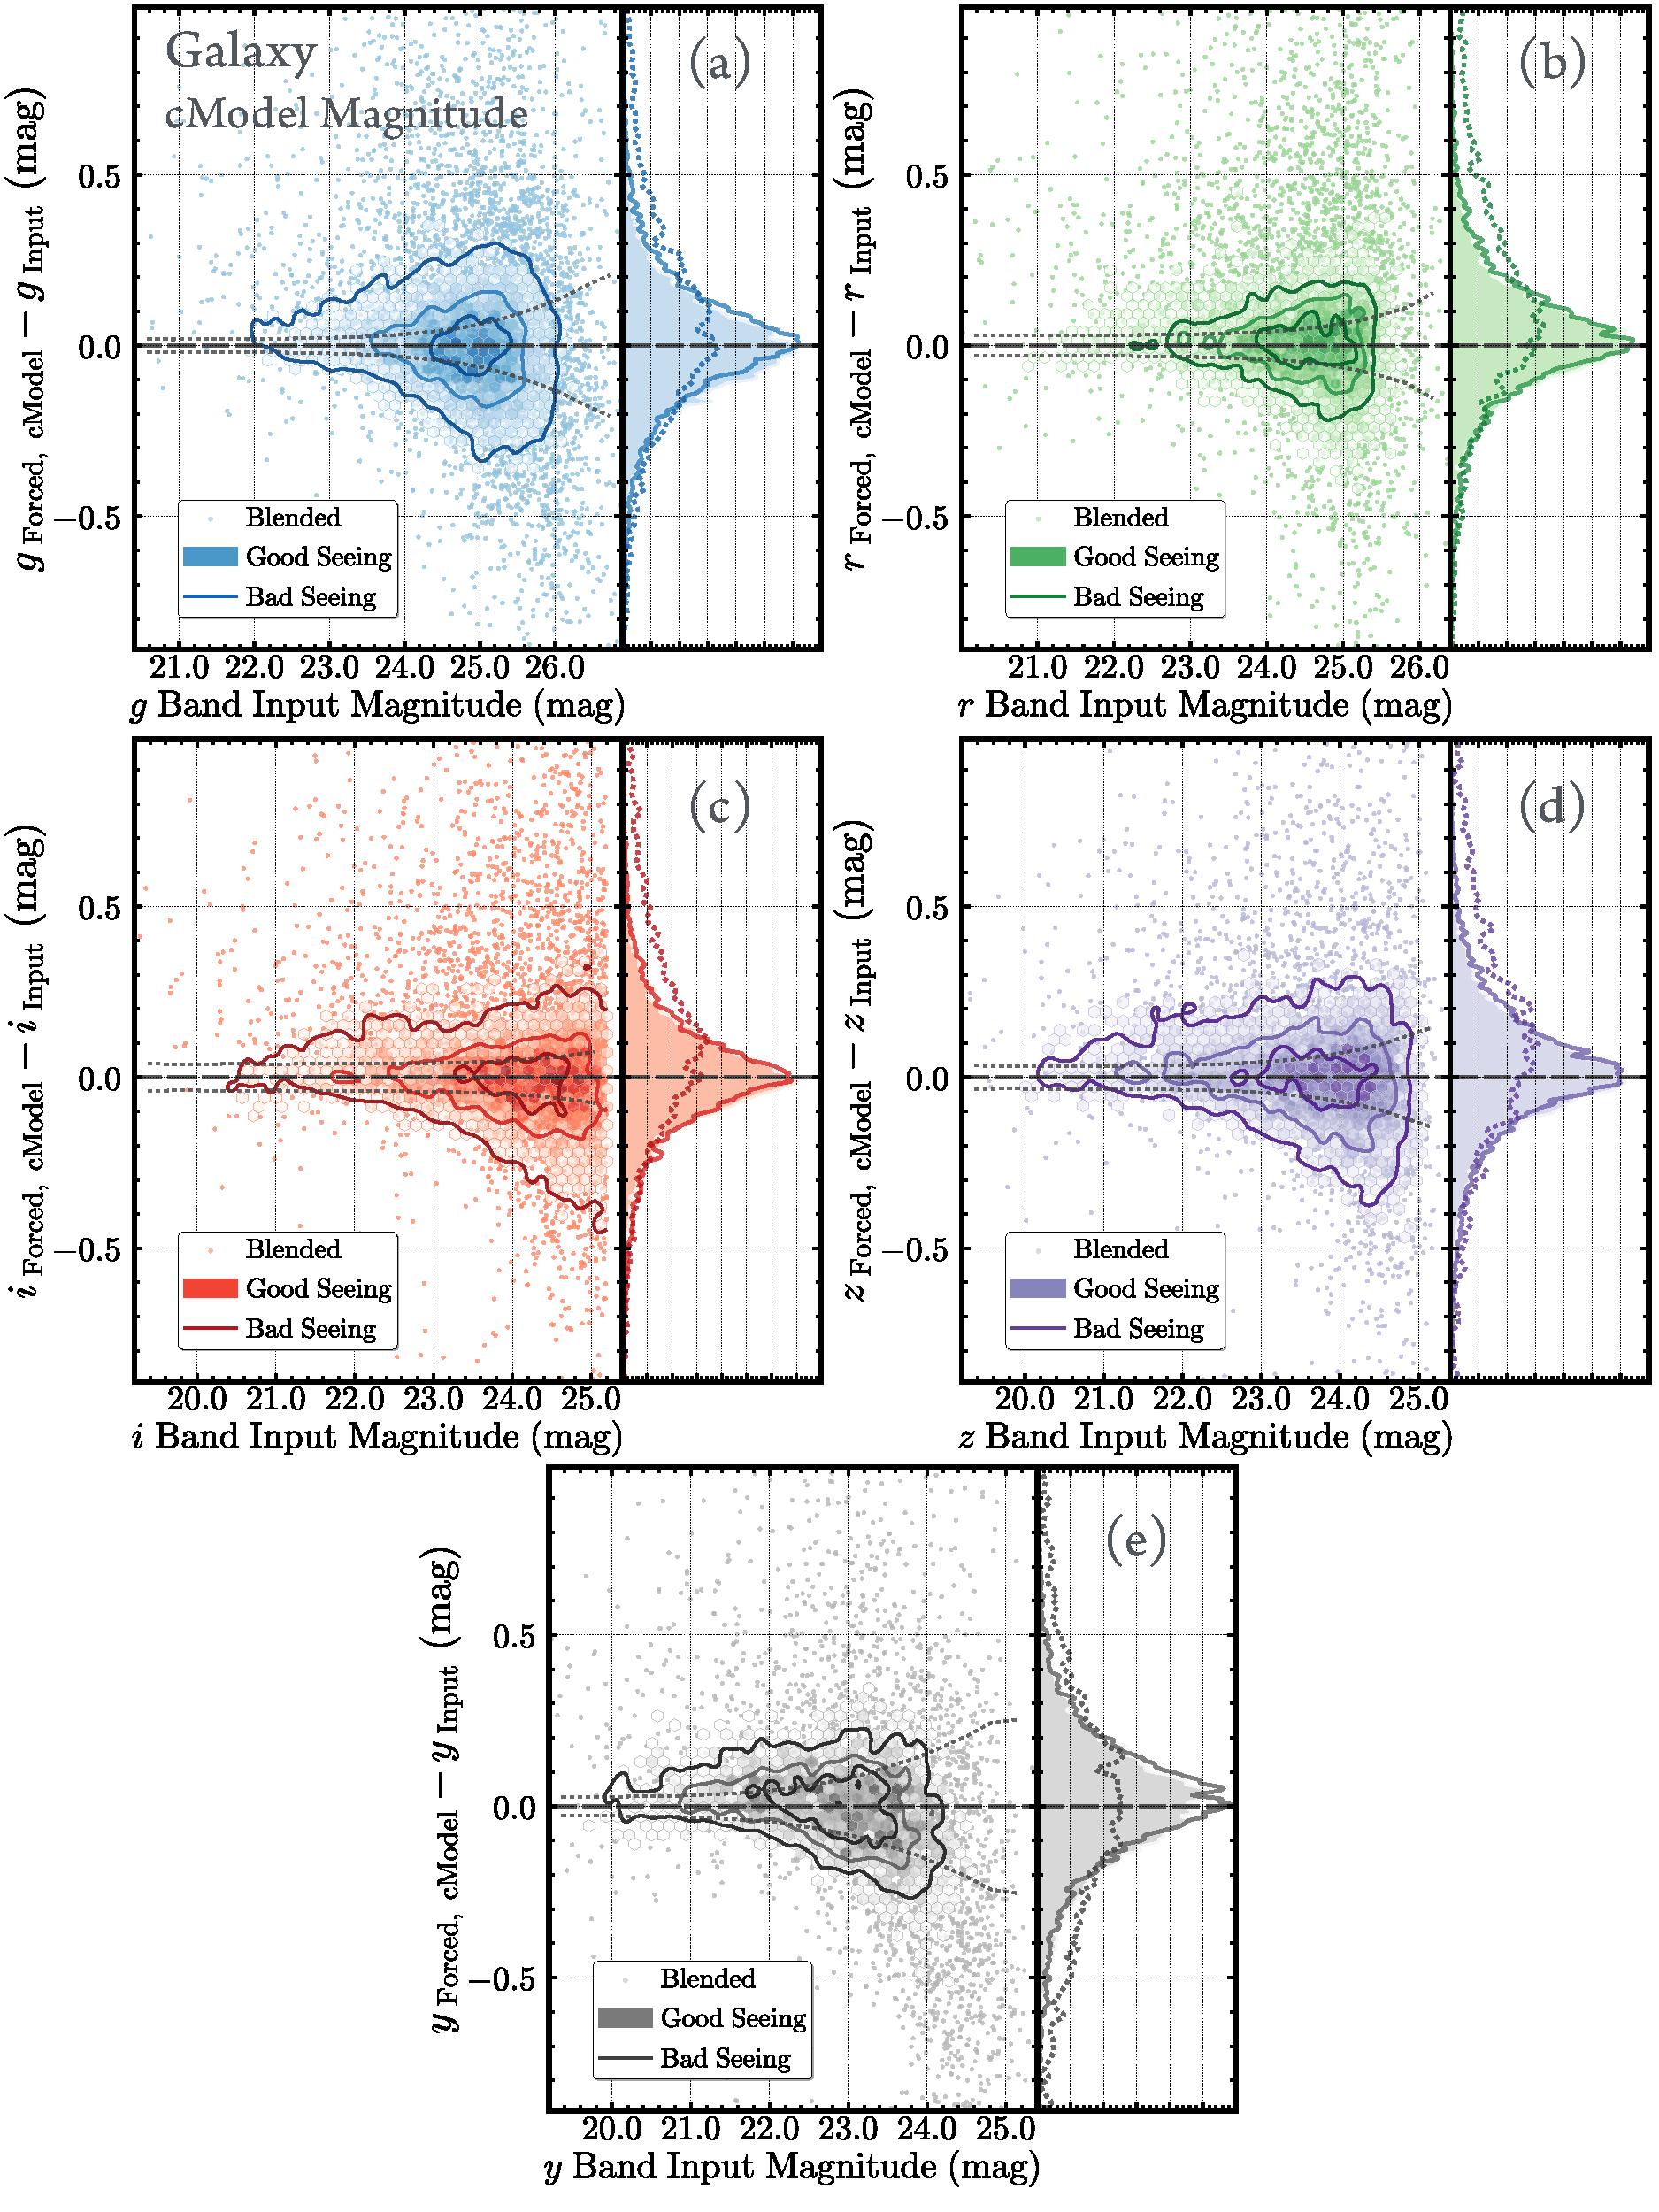
\includegraphics[width=16cm]{fig/synpipe_galaxy_mag}
    \end{center}
    \caption{
        Accuracies of the \texttt{hscpipe} \cmodel{} photometry for synthetic
        galaxies measured by the difference between input and output \forced{}
        \cmodel{} magnitudes.
        Plot [a, b, c, d, e] shows the results for [$g$, $r$, $i$, $z$, $y$]-band.
        Other formats are identical to Fig \ref{fig:psf_mag}.
        }
    \label{fig:cmodel_mag}
\end{figure*}
%% ------------------------------------------------------------------------------------ %%

%% ------------------------------------------------------------------------------------ %%
%% Fig: Difference between the Unforced and Forced Magnitudes
\begin{figure*}
    \begin{center}
        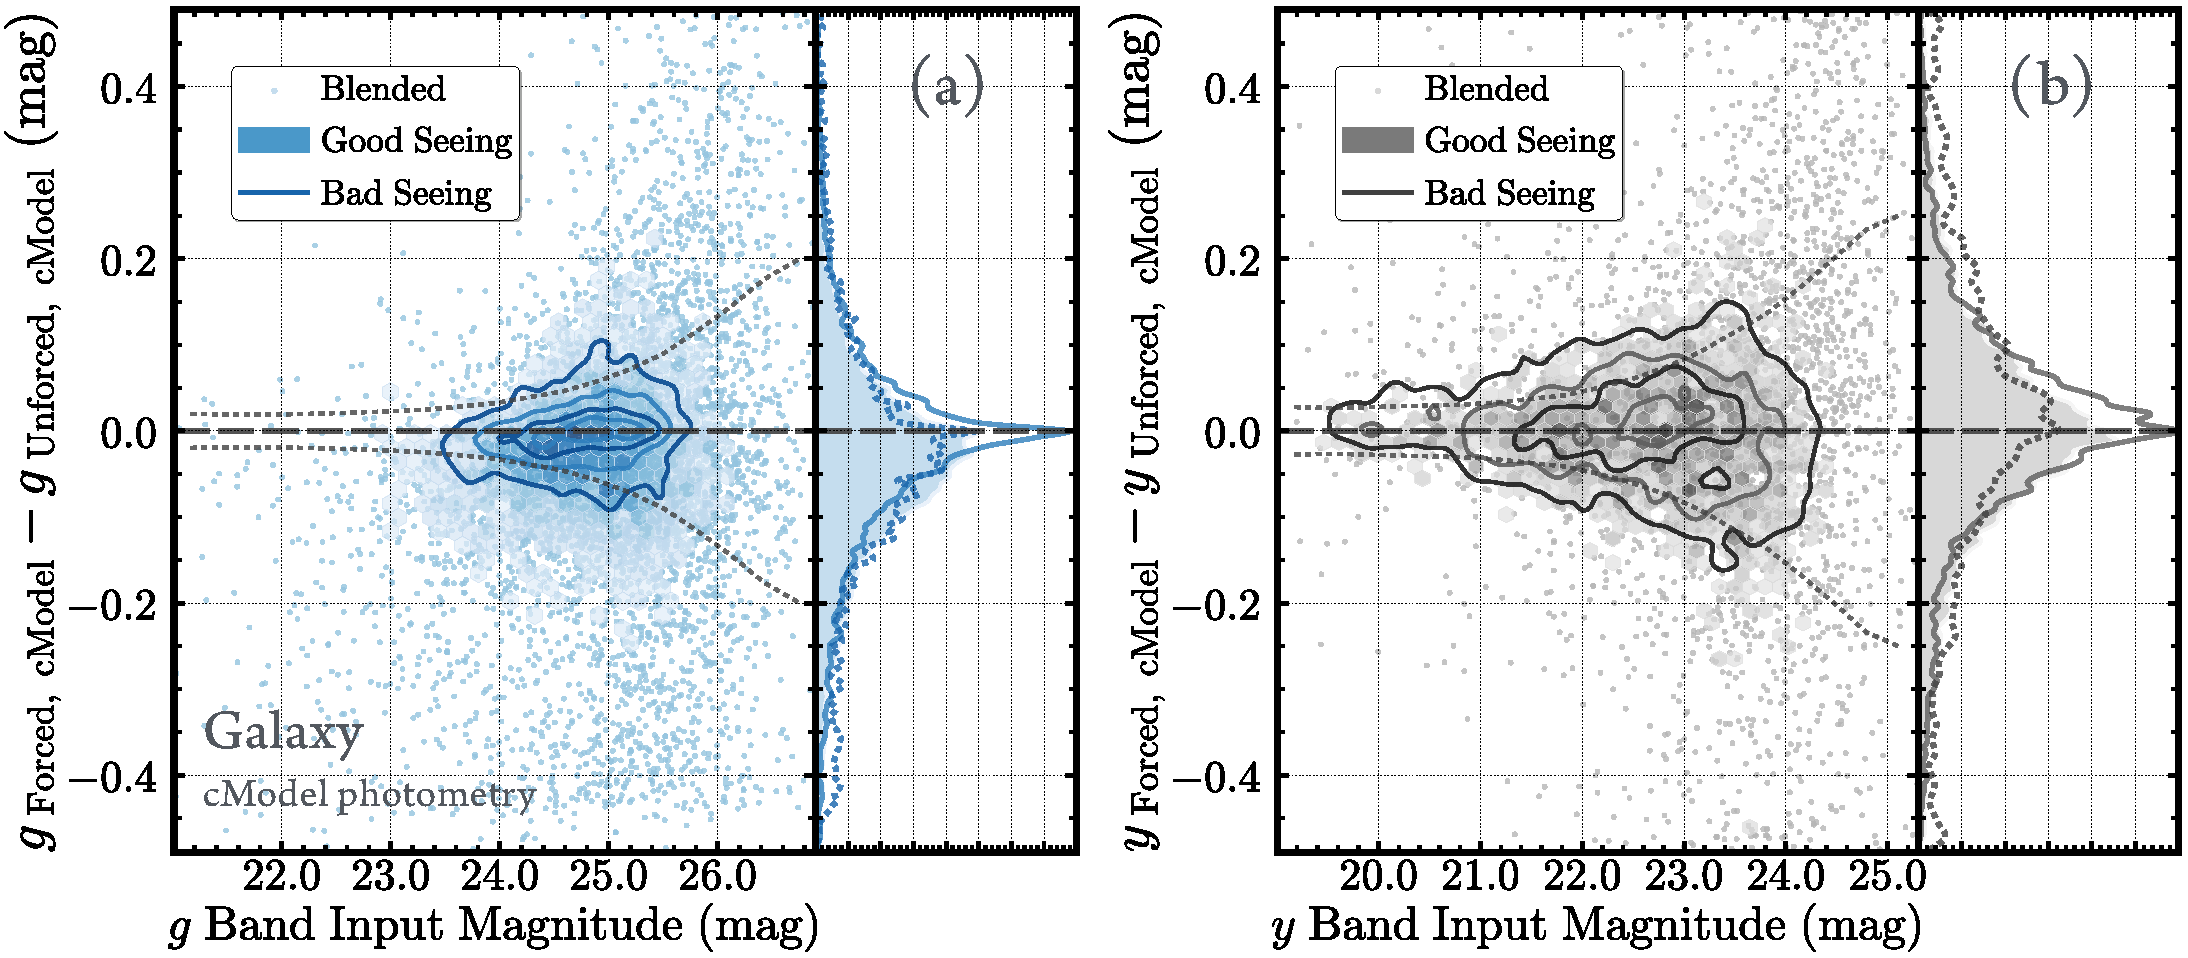
\includegraphics[width=\textwidth]{fig/synpipe_cmodel_diff}
    \end{center}
    \caption{
        The magnitude differences between the \unforced{} and \forced{}
        \cmodel{} photometry for synthetic galaxies in $g$- (\textbf{left} and
        $y$-band (\textbf{right}).
        Other formats are identical to the plots in Fig \ref{fig:psf_diff}.
        }
    \label{fig:cmodel_diff}
\end{figure*}
%% ------------------------------------------------------------------------------------ %%

%% ------------------------------------------------------------------------------------ %%
%% Fig: Accuracies of the cModel color for galaxies
\begin{figure*}
    \begin{center}
        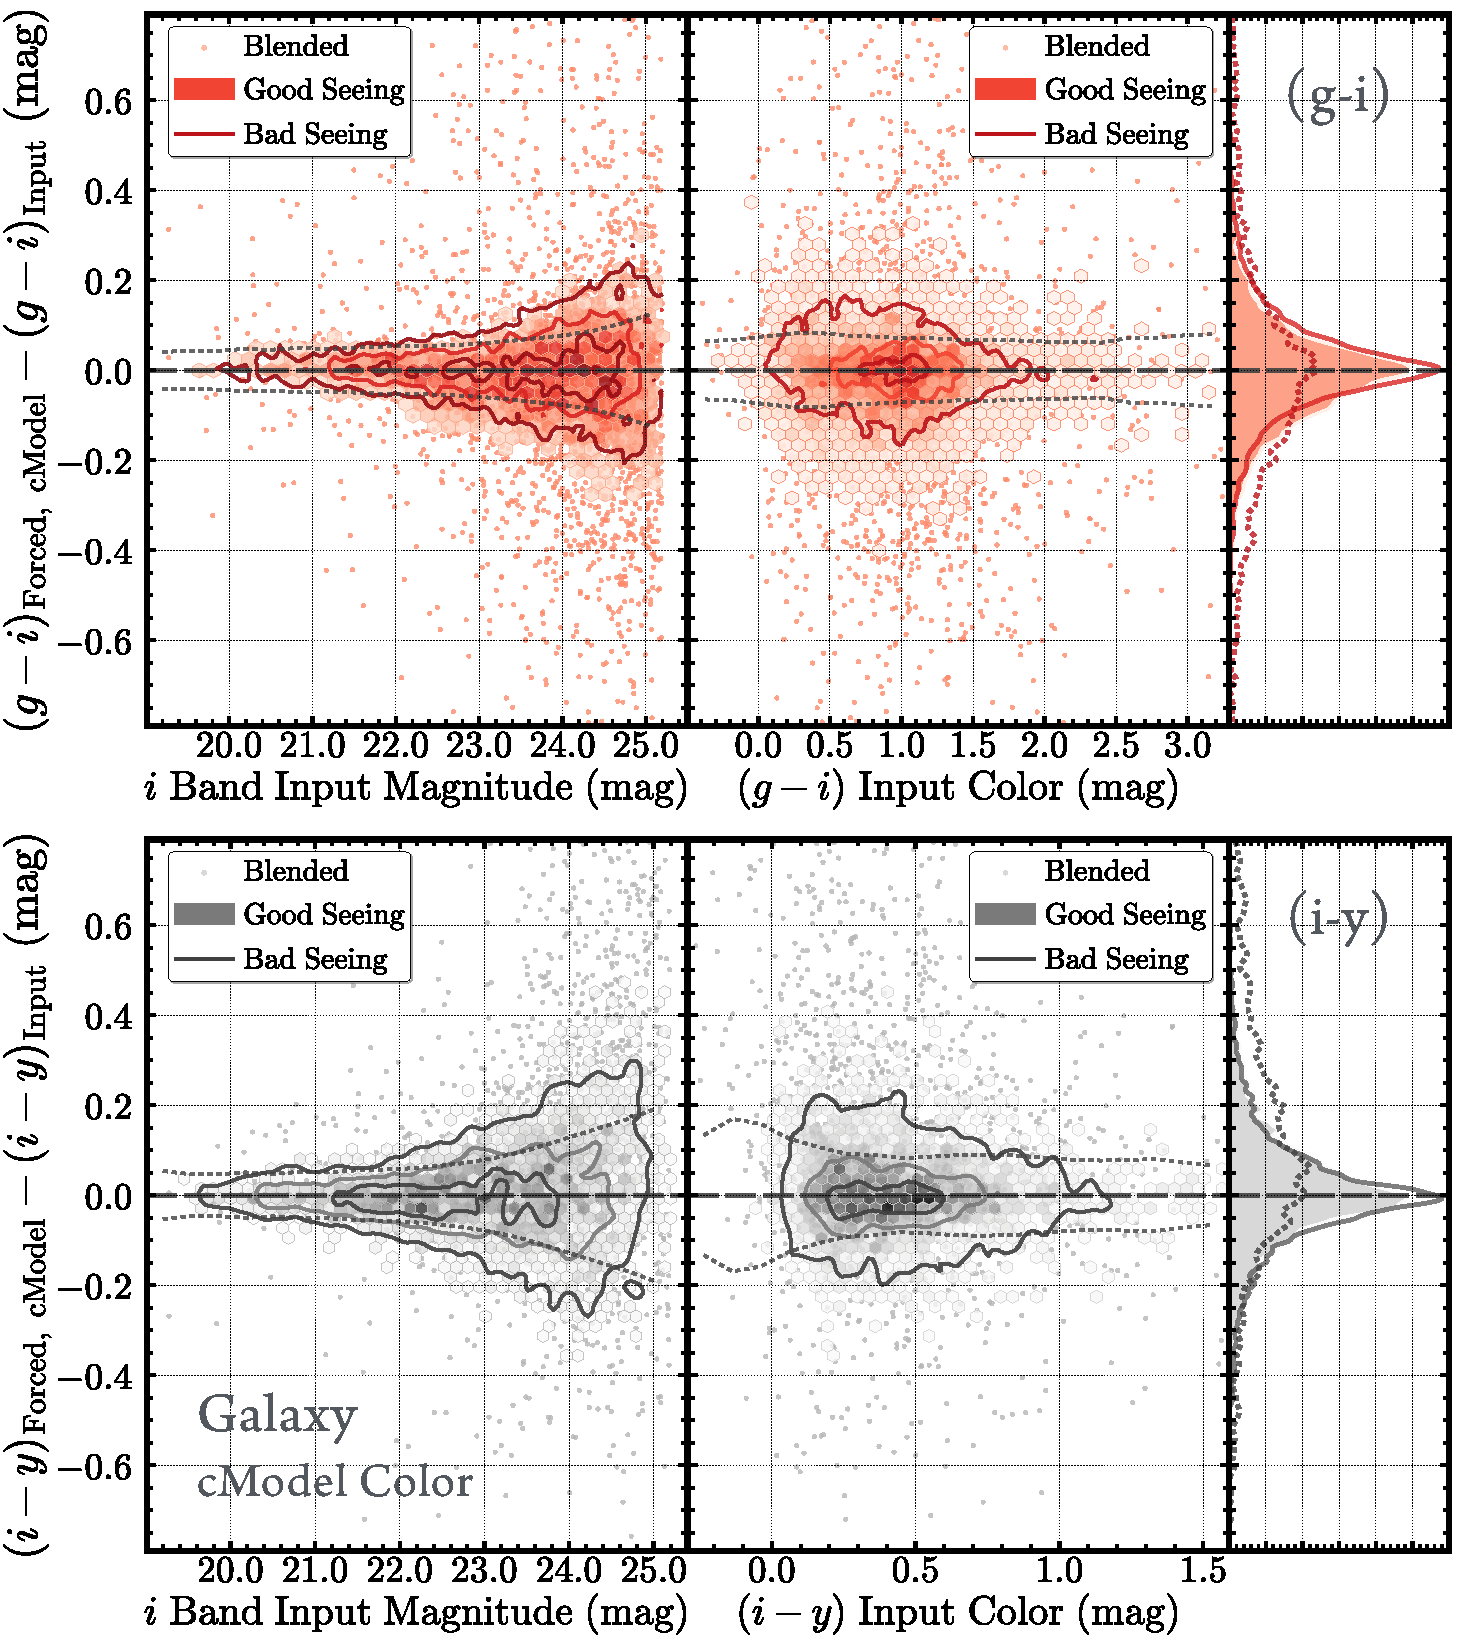
\includegraphics[width=\textwidth]{fig/synpipe_galaxy_color}
    \end{center}
    \caption{
        Accuracies of the color measurements for synthetic galaxies via the
        differences between input and \forced{} \cmodel{} colors.
        The \textbf{Upper panels} and \textbf{lower panels} are for $g-i$ and $i-y$
        colors separately.
        The \textbf{left} column shows the relation between input magnitude and
        the color difference, and the \textbf{right} one uses the input colors as
        x--axis instead.
        Other formats are identical to the plot in Fig \ref{fig:psf_color}.
        }
    \label{fig:cmodel_color}
\end{figure*}
%% ------------------------------------------------------------------------------------ %%

%% ------------------------------------------------------------------------------------ %%
%% Fig: Color-Color Distributions of the Input and Measurements for galaxies
\begin{figure*}
    \begin{center}
        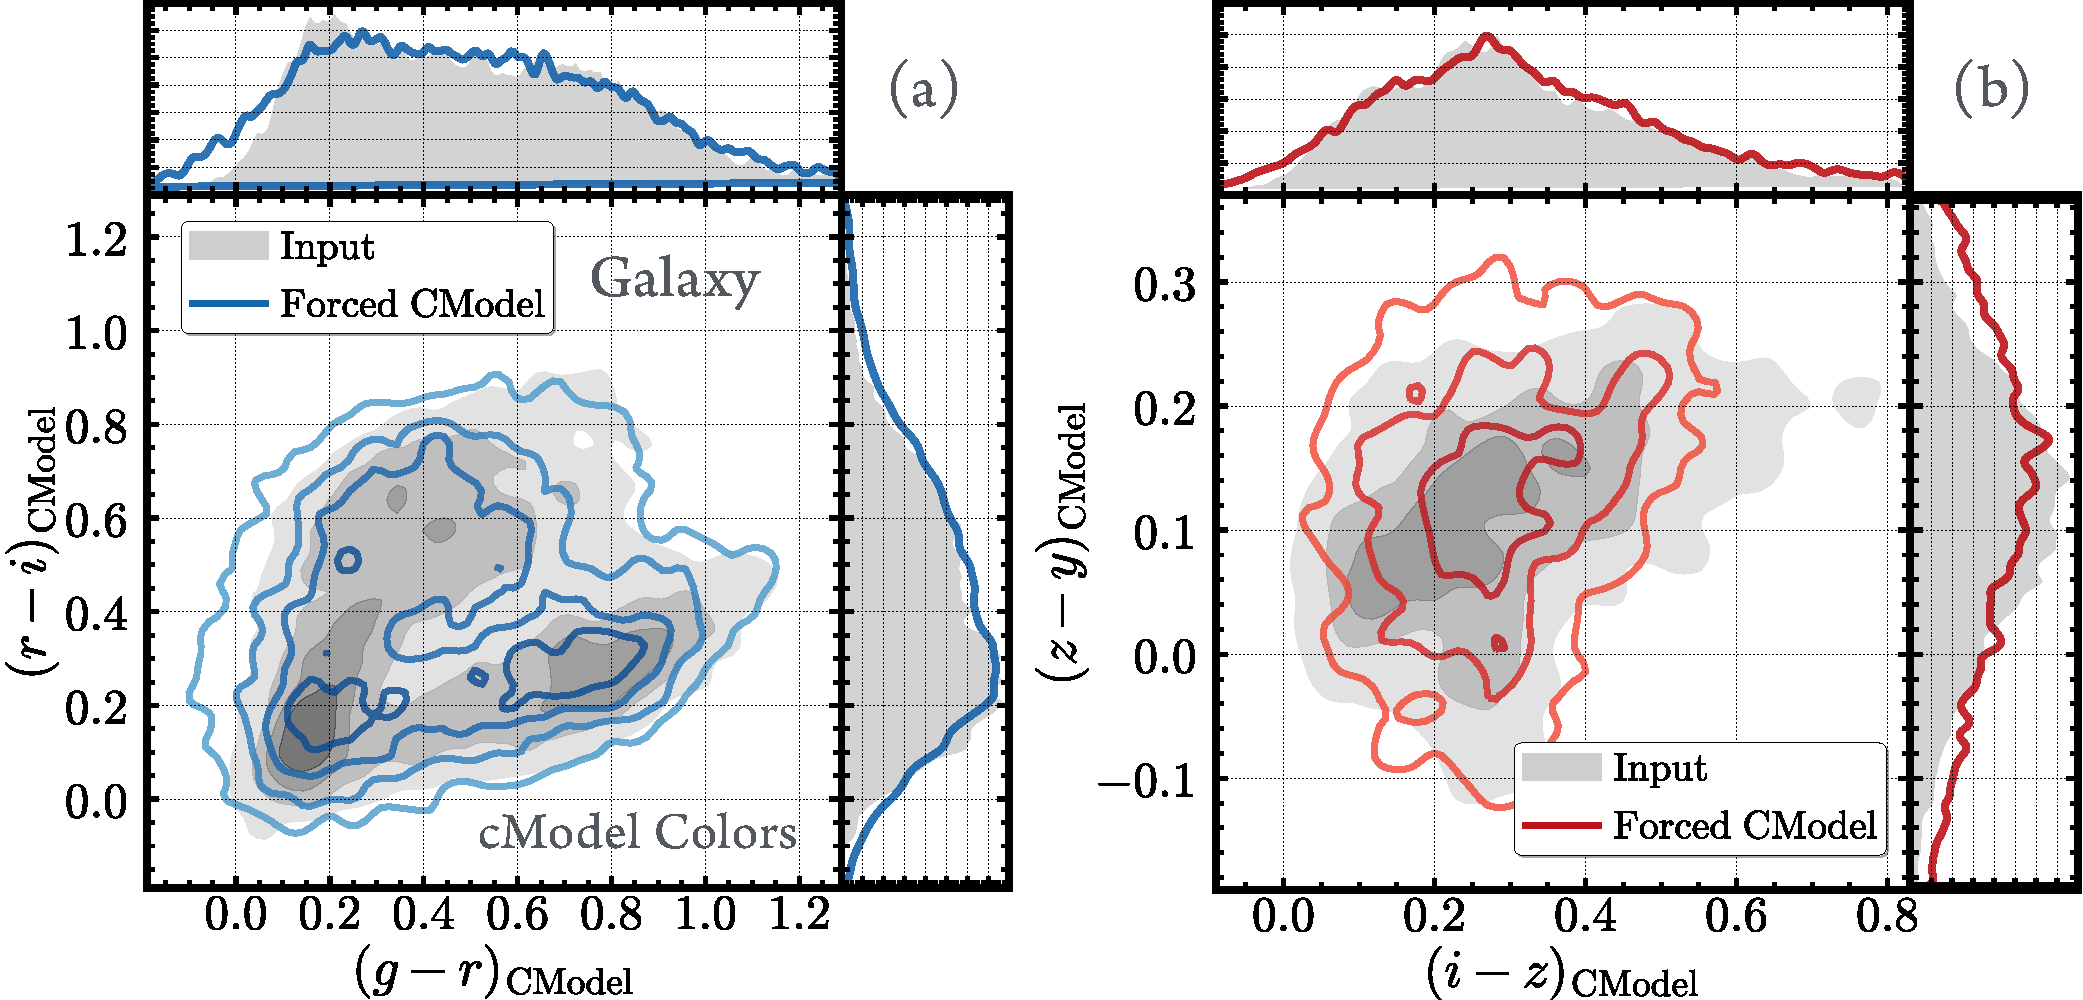
\includegraphics[width=\textwidth]{fig/synpipe_galaxy_cdist}
    \end{center}
    \caption{
        Evaluations of the accuracy of color measurements for synthetic galaxies
        using the color-color distributions.
        \textbf{Left} uses $(g-r)$ v.s. $(r-i)$ colors, and the \textbf{right} one
        uses $(i-z)$ and $(z-y)$ colors.
        The filled contours and shaded histograms reflect the distributions for input
        colors.
        The empty contours and solid-line histograms show the distributions recovered
        by \hscpipe{} \cmodel{} photometry.
        }
    \label{fig:cmodel_cdist}
\end{figure*}
%% ------------------------------------------------------------------------------------ %%

%% ------------------------------------------------------------------------------------ %%
\subsection{cModel photometry of Galaxies}
    \label{ssec:cmodel}

    \cmodel{} algorithm is the primary photometric method for galaxies in
    \hscpipe{} that can be seen as an improved version of the SDSS \cmodel{}
    photometry.
    For more details, please see Section 4.9.8 of Bosch\etal (in prep.).
    In short, \cmodel{} tries to fit each object using a combination of de Vaucouleur
    and exponential profiles that are approximated by multiple Gaussian profiles.
    Despite the limitation of the \cmodel{} method (e.g. sensitive to background
    subtraction and deblender failure), it can deliver robust PSF-corrected fluxes and
    colors for galaxies.

    In our tests, we randomly inject ${\sim}40000$ synthetic galaxies into each 
    \tract{}, and select samples for photometric comparisons in a similar way to the
    stars. 
    First, ${\sim}2$--$3$\% of the synthetic galaxies are ambiguously blended with 
    real objects, and are hence removed from the sample. 
    Among the rest of the sample, ${\sim}2$--$7$\% do not have any match in the 
    \synpipe{} results in different \tracts{} and filters. 
    The fraction of unmatched objects is slightly higher for the $g$- and $y$-band. 
    For the same filter, the fraction is always higher for the bad seeing \tract{}.
    The magnitudes of the unmatched galaxies are systematically fainter than the 
    matched ones. 
    In $i$-band, the median input magnitudes for matched and unmatched galaxies are 
    $24.0$ mag and $24.6$ mag. 
    
    After selecting the matched synthetic galaxies with primary detection and 
    clean photometry (see Appendix \ref{app:qc} for details), we have ${\sim}30000$
    galaxies in each \tract{} for comparison.  
    Among these objects, only $<1$\% is misclassified as point sources by \hscpipe{}
    in the good seeing \tract{}.  
    However, for the bad seeing one, the fraction increases to $4$\%.  
    The median input magnitude for these misclassified sources is ${\sim}24.9$ mag 
    in $i$-band, significantly fainter than the median of others.  
    We will further discuss this in Section \ref{ssec:sg}.
    
    We also use $b>0.1$ to define samples of highly blended galaxies.
    Due to the extended nature, the distributions of $b$ for synthetic galaxies are 
    very different from stars, and skew toward higher values (especially for the 
    bad-seeing \tract{}). 
    About ${\sim}7$--$9$\% of synthetic galaxies are highly blended by this standard.
    The fraction is only slightly higher in the bad-seeing \tract{}, and the 
    $g$-band has the highest fraction of highly blended galaxies. 
    We highlight the highly blended ones in comparisons, and there are more relevant 
    discussions in Section \ref{ssec:blendedness}.
    
    Although these galaxies span in very wide large ranges of magnitude and 
    structural parameters, the majority of them are faint 
    ($i_{\mathrm{Input}} > 24.0$ mag) and small ($R_{\mathrm{e}} < 0.5$\asec). 
    The photometric quality of these galaxies is very challenging, and also crucial
    to several key scientific goals of the HSC survey. 
    At the same time, these samples are unable to provide enough amounts of 
    bright or large galaxies to test. 
    We will supplement results for these galaxies using better samples for them 
    in the future. 

%% ------------------------------------------------------------------------------------ %%
\subsubsection{Input magnitude and the \s2n{} of \cmodel{} photometry}

    In Fig \ref{fig:cmodel_sn}, we first show the relations between the input 
    magnitudes and the \s2n{} of the synthetic galaxies estimated by the ratio 
    between \cmodel{} flux and its uncertainties from \hscpipe{}. 
    Since these galaxies are extended objects, the \s2n{} here should be treated 
    as the average \s2n{} which is different from the \s2n{} of stars using PSF 
    photometry. 
    
    We still use $i$- and $g$-band as examples. 
    Comparing to the similar figure for stars, the most obvious difference is that
    at fixed input magnitude, the \s2n{} distribution of galaxies show much larger
    scatter than stars.  
    At the same total flux, galaxy can have different size and shape, and 
    naturally leads to differences in their peak and average \s2n{}.  
    This also makes it difficult to have a clear definition of ``detection limit'' 
    for galaxies. 
    For $i$-band, the typical \s2n{} for synthetic galaxies at the magnitude limit 
    of our sample ($25.2$ mag) is ${\sim}20$, but the low-\s2n{} tail has already 
    reached to the \s2n{}$=5$ boundary.  
    This suggests that, although HSC Wide can detect galaxies as faint as 
    $i{\sim}26.0$ mag, the sample will become highly incomplete. 
    Furthermore, it can also introduce bias into the selection as galaxies with 
    certain structural properties are harder to detect than others. 
    Users of HSC survey data who want to select flux-limited samples of galaxies,
    or intend to study the population of faint (e.g. high-$z$) galaxies should
    keep this in mind.  
    
    Similar to the synthetic stars, worse seeing condition can also lead to 
    noticeable decrease of \s2n{} at the same magnitude (see the figure for
    $i$-band). 
    Meanwhile, the highly blended synthetic galaxies do not show significantly 
    different \s2n{} distributions here. 

%% ------------------------------------------------------------------------------------ %%
\subsubsection{Accuracy of the \cmodel{} magnitude}

    In Fig \ref{fig:cmodel_mag}, we illustrate the photometric uncertainties of the 
    \cmodel{} magnitudes in each band using the same format with 
    Fig \ref{fig:psf_mag}.
    
    The overall performance of \cmodel{} photometry is very reasonable all the way 
    down to $i_{\mathrm{Input}}=25.2$ mag. 
    Comparing to the qualities of PSF photometry for stars, the magnitude differences
    of \cmodel{} show much larger scatter. 
    Given the diversity of properties of these galaxies and the complexities in the 
    model-fitting process, this difference is expected.  
    At the same time, we can see that the \cmodel{} algorithm in \hscpipe{} can 
    provide unbiased and consistent photometry for galaxies in different bands and 
    seeing conditions. 
    
    In $i$-band, the median flux uncertainties of \forced{} \cmodel{} is ${\sim}7$\% 
    in the good-seeing \tract{} at $i_{\mathrm{Input}}{\sim}20.0$ mag, 
    and ${\sim}9$\% at $i_{\mathrm{Input}}{\sim}24.0$ mag.  
    Down to $i_{\mathrm{Input}}{\sim}25.0$ mag, the median uncertainty maintains 
    at ${\sim}11$\% level. 
    For the bad-seeing \tract{}, the performance is very similar in $i$-band. 
    From $i_{\mathrm{Input}}{\sim}20.0$ to $25.0$ mag, the median magnitude difference
    between output and input values changes from \plus{}$0.041$ mag to 
    \minus{}$0.005$ mag, which suggests that \forced{} \cmodel{} photometry is 
    unbiased down to very faint end. 
    It is worth noting that the photometric uncertainties estimated by \synpipe{}
    are significantly larger than the fiducial error from \hscpipe{} that does not 
    take into account the systematically uncertainties involved in the modeling 
    fitting process. 
    Although the synthetic galaxies here are described by the simple single-\ser{} 
    model, \cmodel{} algorithm can only approximate them to certain accuracy, 
    especially when the noise level, deblending uncertainty, and priors of model 
    parameters are considered. 
    Given that the real galaxies are more complex in structural details, these 
    uncertainties should be treated as lower limits. 
    
    The performance of \forced{} \cmodel{} photometry is very consistent across all
    filters. 
    For $g$, $r$, and $z$-band, the photometric uncertainties are very similar to 
    the ones for $i$-band between $20.0$ to $25.0$ mag. 
    The \forced{} \cmodel{} magnitudes are also unbiased for these 3 filters 
    across the entire input magnitude range. 
    The uncertainties for $y$-band are slightly large, range from 9-17\% in the 
    same magnitude bins. 
    In addition, \forced{} \cmodel{} tends to overestimate the total flux in $y$-band
    at $y_{\mathrm{Input}}>24.0$ mag. 
    Mean magnitude differences change from \minus{}0.06 at 24.0 mag to \minus{}0.22
    mag at 25.0 mag.  
    Both worse seeing condition and higher background noise level can make it more 
    difficult to detect faint object on $y$-band image.
    At $y_{\mathrm{Input}}{\sim}24.0$, the average \s2n{} for \cmodel{} in $y$-band
    is already close to the detection threshold. 
    
    As mentioned, the statistics for brighter galaxies are very uncertain due to 
    small sample size. 
    However, we do notice that, at $i_{\mathrm{Input}}<20.0$, the \forced{} 
    \cmodel{} photometry shows larger uncertainty and starts to systematically 
    underestimate the total flux.  
    This problem is confirmed via comparing with more carefully derived total fluxes 
    for bright galaxies (e.g. \citealt{HSCDR1}, Huang\etal in prep.). 
    It relates to the known issues of \hscpipe{} (e.g. over-deblend around bright 
    objects; inappropriate weighting of priors in \cmodel{}), but it may also suggest
    that, at the imaging depth of HSC, assumptions in \cmodel{} are no longer the 
    best choice in modeling these galaxies (e.g. for massive elliptical galaxies; 
    see Huang\etal in prep.~for more details). 
    
    For the highly blended synthetic galaxies, we also see systematically 
    underestimated total flux (average offset ${\sim}0.1$ mag) and larger scatter 
    of photometric uncertainty in all five bands.  
    Meanwhile, the contrast between relative isolated and highly blended galaxies 
    in photometric performance is no longer as staggering as the one for synthetic
    stars (Fig \ref{fig:psf_mag}).
    
    We also test the \unforced{} \cmodel{} photometry in all five bands, and the 
    results suggest similar accuracies.
    We highlight the differences between \forced{} and \unforced{} \cmodel{} 
    photometry in $g$- and $y$-band in Fig \ref{fig:cmodel_diff}.
    The only noticeable difference is for galaxies brighter than $24.0$ mag in 
    $g$-band, their \forced{} \cmodel{} magnitudes are systematically brighter than 
    the \unforced{} ones. 
 
%% ------------------------------------------------------------------------------------ %%   
\subsubsection{Accuracy of the \cmodel{} color}

    The consistent and accurate five-band \cmodel{} colors from \hscpipe{} are crucial 
    to the photometric redshift and spectral energy distribution (SED) fitting results. 
    They are also key to the selection of high-$z$ Lyman-break galaxies (LBG) and 
    and many other interesting objects. 

    In Fig \ref{fig:cmodel_color}, we demonstrate the accuracies of \forced{} $(g-i)$
    and $(i-y)$ \cmodel{} colors in the same format for synthetic stars 
    (Fig \ref{fig:psf_color}).
    These plots show that \hscpipe{} can provide reliable \cmodel{} colors for 
    synthetic galaxies down to $i_{\mathrm{Input}}{\sim}25.0$ mag. 
    For $(g-i)$ colors, average uncertainty around $i_{\mathrm{Input}}{\sim}21.0$ mag 
    is ${\sim}0.04$ mag.
    The uncertainty increases to ${\sim}0.11$ mag at $i_{\mathrm{Input}}{\sim}25.0$ mag.
    Results for $(i-y)$ colors are similar.
    
    The performance of \forced{} \cmodel{} color does not show dependence on seeing
    condition, and is unbiased across the ranges for input total magnitude and color.
    The only noticeable feature is that the $(i-y)$ color at 
    $i_{\mathrm{Input}}>24.0$ is slightly overestimated. 
    As mentioned above, this is not surprise given the shallower imaging depth of 
    $y$-band.    
    At the same time, high blendedness of synthetic galaxies can still increase the 
    uncertainties of the color and bias the color measurements.
    The highly blended galaxies on average show slightly bluer $(g-i)$ 
    colors and redder $(i-y)$ colors than the input values.
    
    Similar to Fig \ref{fig:psf_cdist}, we also compare the color--color distributions 
    of the input and output \forced{} \cmodel{} values in Fig \ref{fig:cmodel_cdist}. 
    The general distributions of colors are well recovered despite the accuracy is 
    not as good as the one for stars, especially on the $(i-z)$ v.s. $(z-y)$ plane. 
    It is expected given the narrow dynamical ranges of these colors among red filters.
    The \forced{} \cmodel{} tends to slightly underestimate the $(g-r)$ and $(i-z)$ 
    colors at the very ``blue'' end, while overestimate the $(i-y)$ color at very 
    red end. 
    
    In the end, we should point out that we assume constant color for the entire galaxy.  
    In reality, different colors for individual components and smooth color gradient 
    can really complicated the situation, hence the uncertainties of \cmodel{} colors 
    here should be considered as lower limits.
%% ------------------------------------------------------------------------------------ %%


%% ------------------------------------------------------------------------------------ %%
%% Fig: Astrometric Calibration
\begin{figure*}
    \begin{center}
        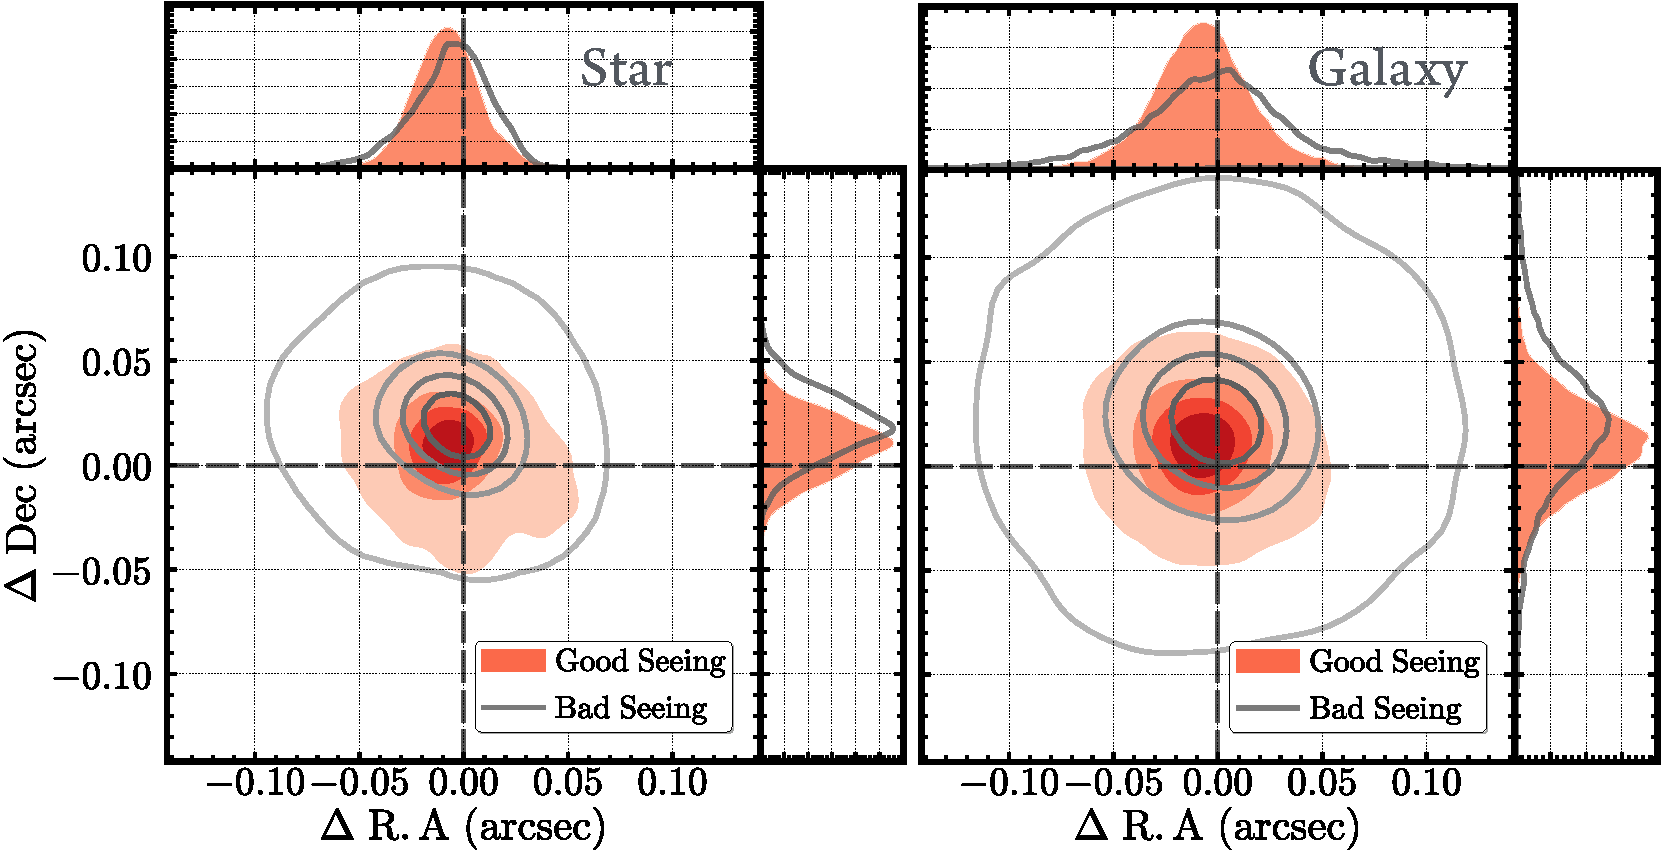
\includegraphics[width=\textwidth]{fig/synpipe_astrometry}
    \end{center}
    \caption{
        Astrometric accuracy for synthetic star (\textbf{left}) and galaxy
        (\textbf{right}) via the differences in R.A and Dec between the input
        coordinates and the ones measured on the coadd images.
        Hexagonal bins (filled histogram) and contours (solid-line histogram) are for
        the synthetic objects from \tracts{} with good and bad seeing conditions.
        $\Delta\mathrm{R.A}=0$ and $\Delta\mathrm{Dec}=0$ are marked by dashed lines.
        }
    \label{fig:astrometry}
\end{figure*}
%% ------------------------------------------------------------------------------------ %%


%% ------------------------------------------------------------------------------------ %%
%% Fig: Star-Galaxy Separation
\begin{figure*}
    \begin{center}
        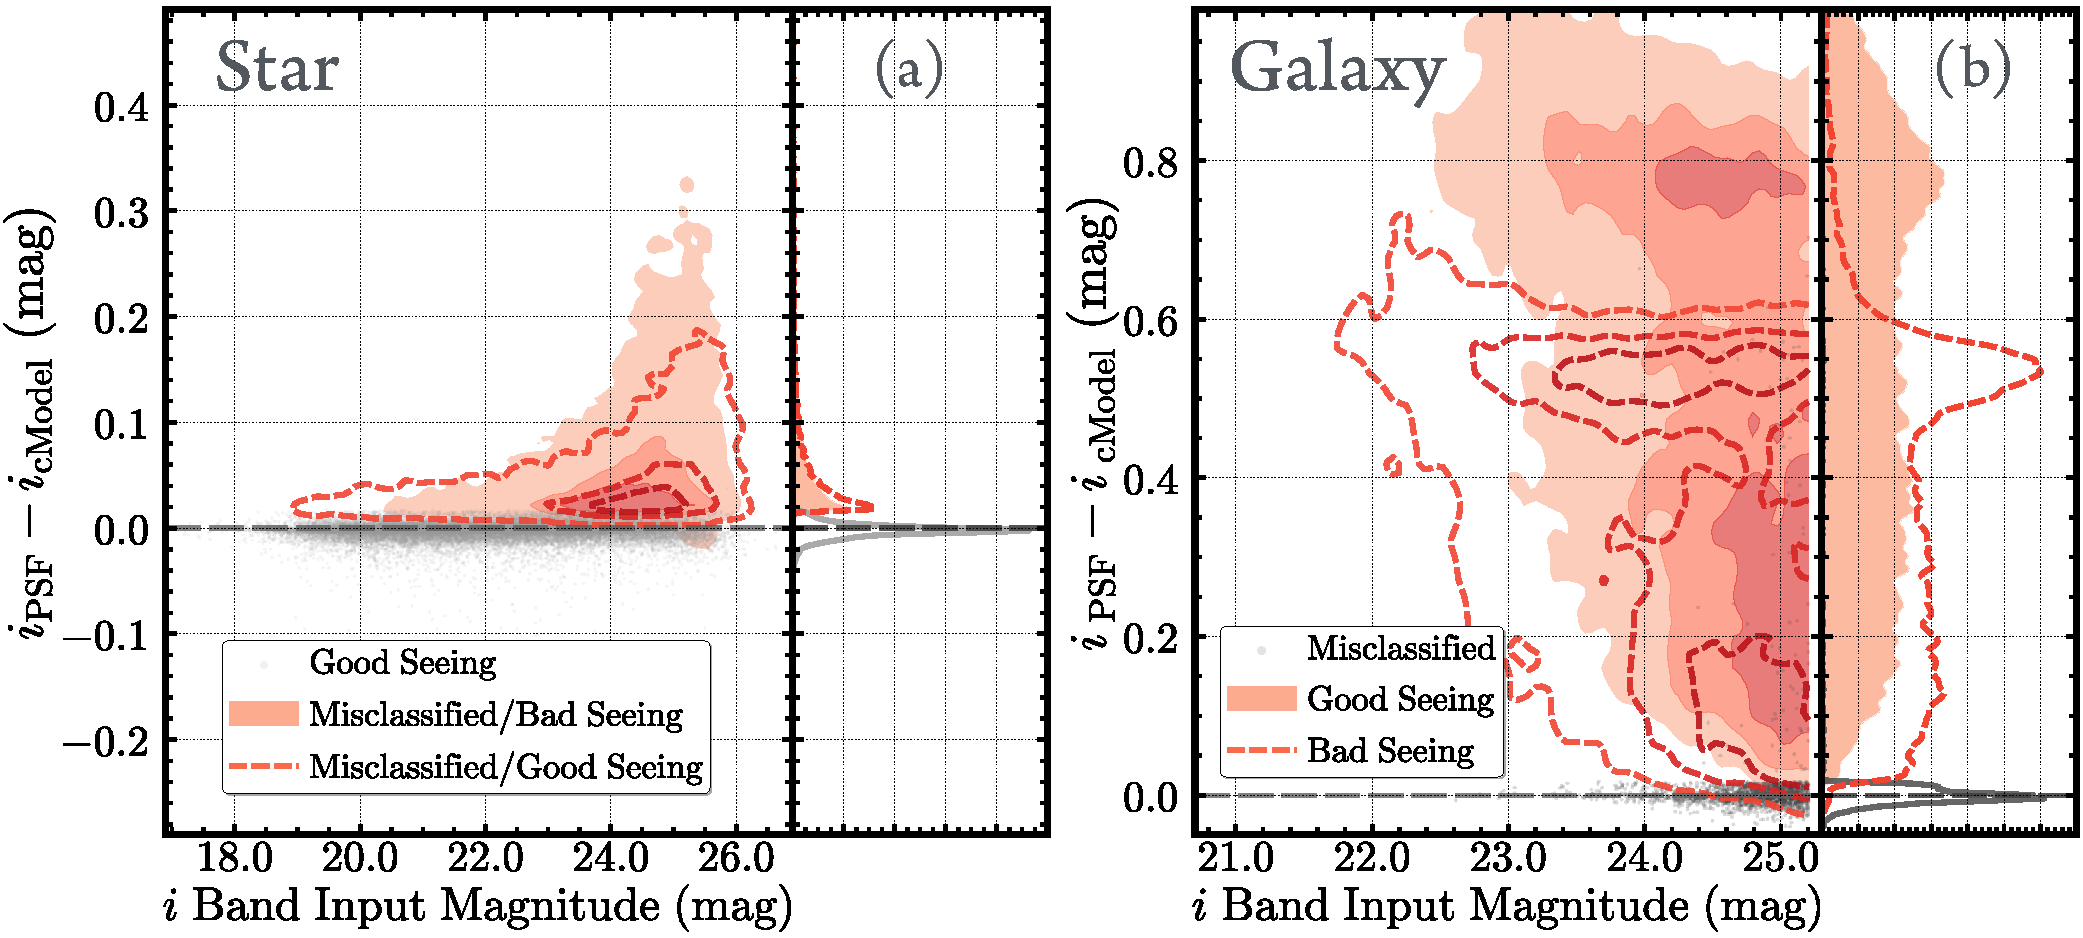
\includegraphics[width=\textwidth]{fig/synpipe_star_galaxy}
    \end{center}
    \caption{
        Illustrates the problems with current star--galaxy separation method in
        \hscpipe{} which is based on the magnitude difference between the PSF and
        \cmodel{} photometry.
        \textbf{Left} plot is for the synthetic stars.
        Hexagonal bins and filled histogram show distributions of correctly classified
        synthetic stars in the good seeing \tract{}.
        The scatter plot (dashed-line histogram) and contour (solid-line histogram)
        show distributions of synthetic stars that are misclassified as extended
        objects in \tracts{} with bad and good seeing conditions.
        \textbf{Right} one is for synthetic galaxies.
        Here the hexagonal bins (filled histogram) and contours (solid-line histogram)
        are for galaxies from good and bad seeing \tracts{}.
        The scatter plot and dashed-line histogram are for synthetic galaxies that are
        misclassified as point sources.
        Zero magnitude difference is highlighted using dashed lines on both plots.
        }
    \label{fig:sg}
\end{figure*}
%% ------------------------------------------------------------------------------------ %%

%% ------------------------------------------------------------------------------------ %%
%% Fig: Relations between Blendedness and Photomertic Errors
\begin{figure*}
    \begin{center}
        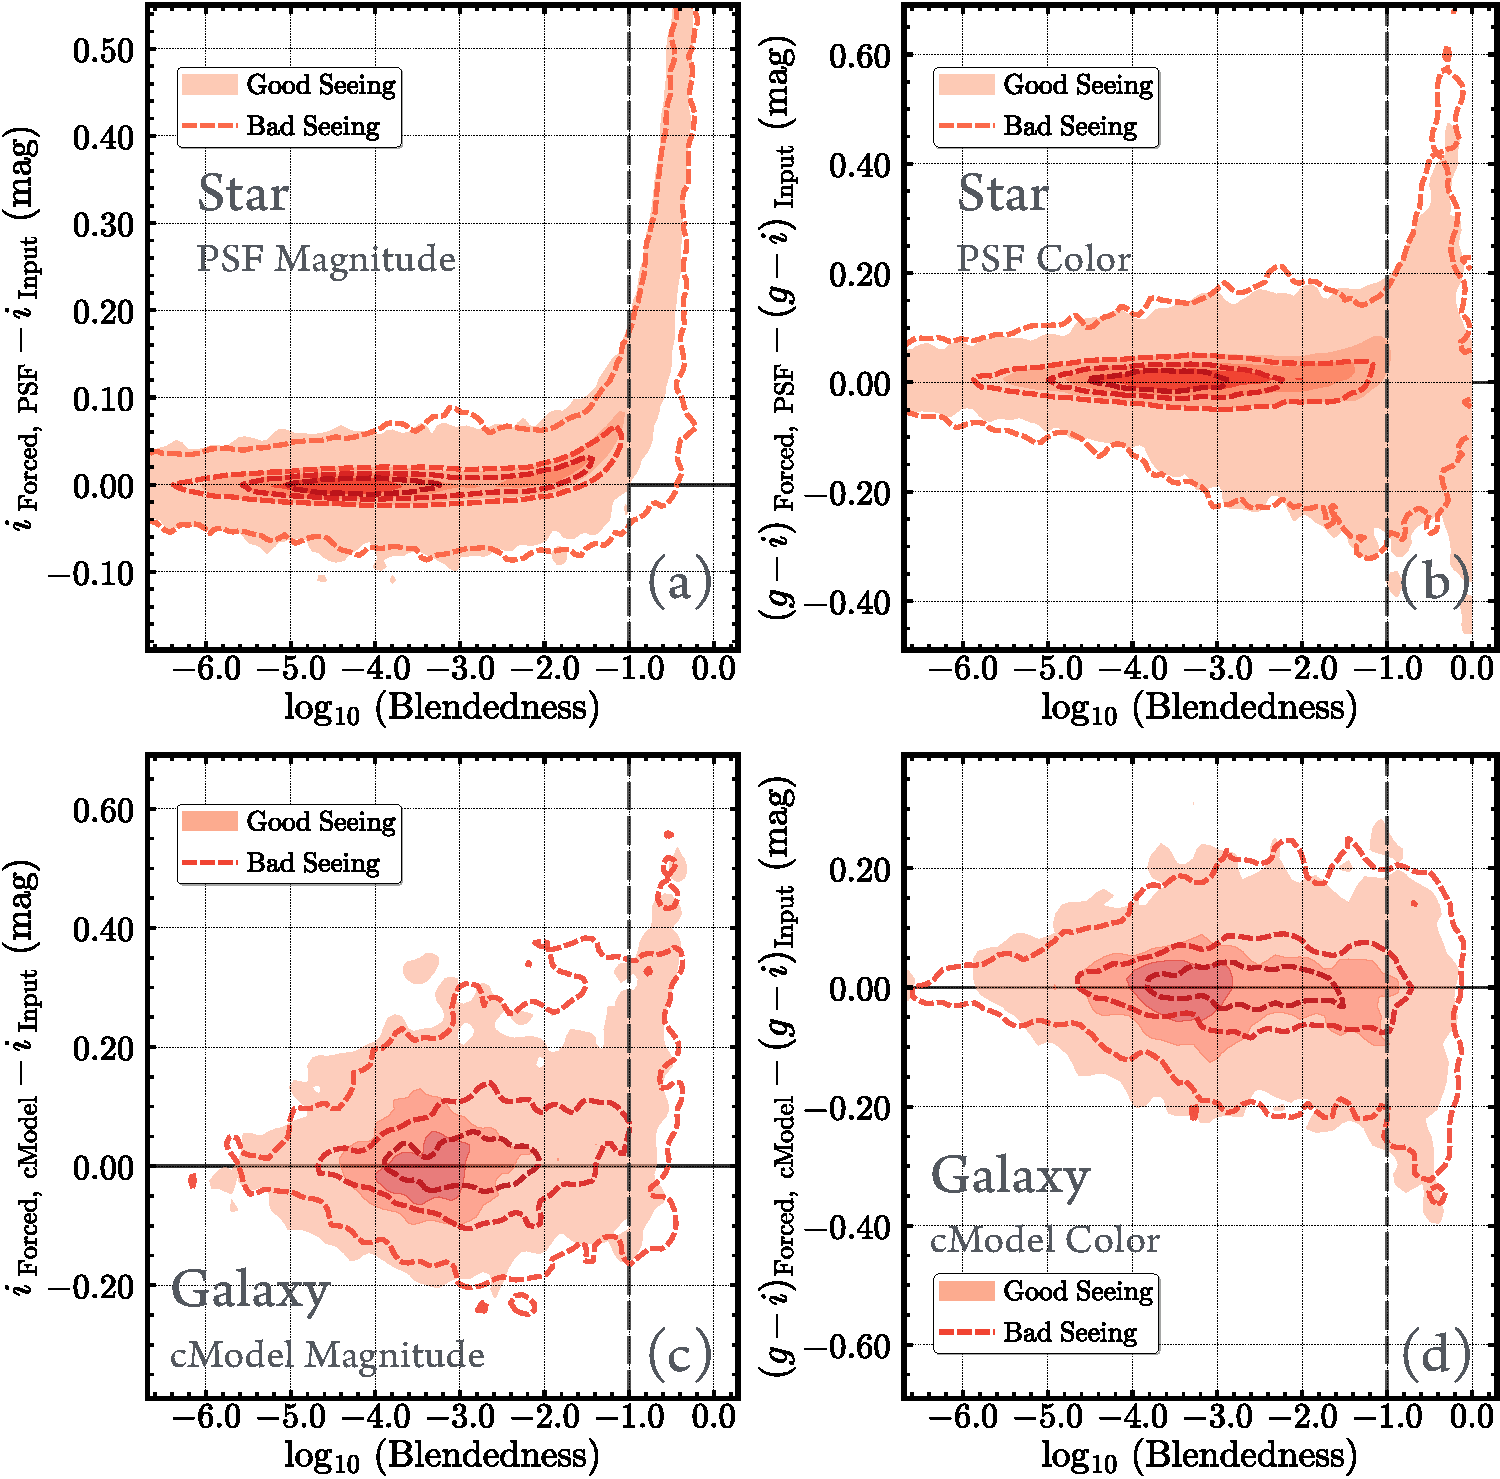
\includegraphics[width=\textwidth]{fig/synpipe_blendedness_err}
    \end{center}
    \caption{
        Shows the relationships between the $\log(\mathrm{Blendedness})$ parameter
        and the photometric accuracies for synthetic stars (\textbf{upper row}) and
        galaxies (\textbf{lower row}).
        \textbf{Left} column is for uncertainties of PSF or \cmodel{} magnitude,
        and the \textbf{right} one is for uncertainties of $(g-i)$ color.
        Hexagonal bins and contours show results for good and bad seeing
        \tracts{}.
        $\log(\mathrm{Blendedness}) = -1.0$ is marked using vertical dashed line.
        }
    \label{fig:blend}
\end{figure*}
%% ------------------------------------------------------------------------------------ %%

%% ------------------------------------------------------------------------------------ %%
%% Fig: Compare with the behaviours of the Kron photometry for galaxies
\begin{figure*}
    \begin{center}
        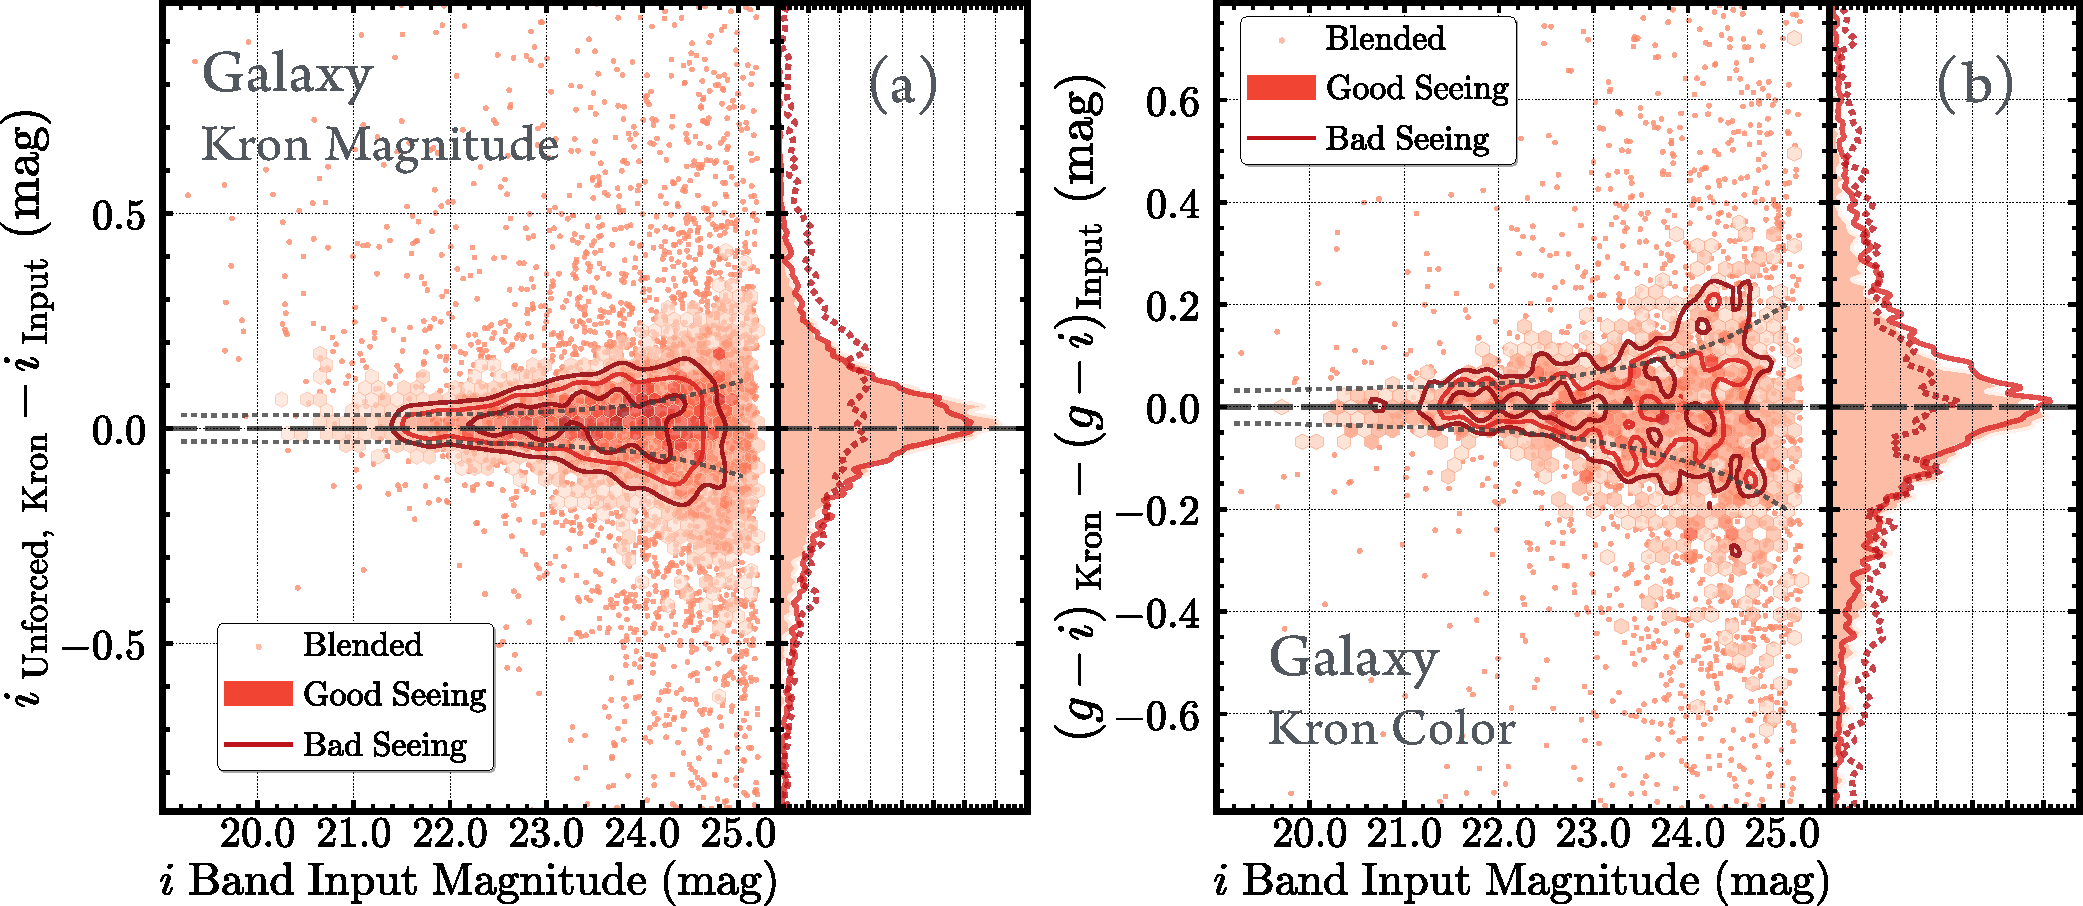
\includegraphics[width=\textwidth]{fig/synpipe_galaxy_kron}
    \end{center}
    \caption{
        Basic performance of the Kron photometry for synthetic galaxies.
        \textbf{Left} shows the accuracy in $i$-band.
        magnitude. The format is identical to Fig \ref{fig:galaxy_mag}.
        \textbf{Right} shows the accuracy of the $(g-i)$ color using
        Kron photometry.
        Other formats are identical to Fig \ref{fig:cmodel_color}.
        }
    \label{fig:galaxy_kron}
\end{figure*}
%% ------------------------------------------------------------------------------------ %%

%% ------------------------------------------------------------------------------------ %%
%% Fig: HSC cModel has problem recovering the size and shape of galaxies
\begin{figure*}
    \begin{center}
        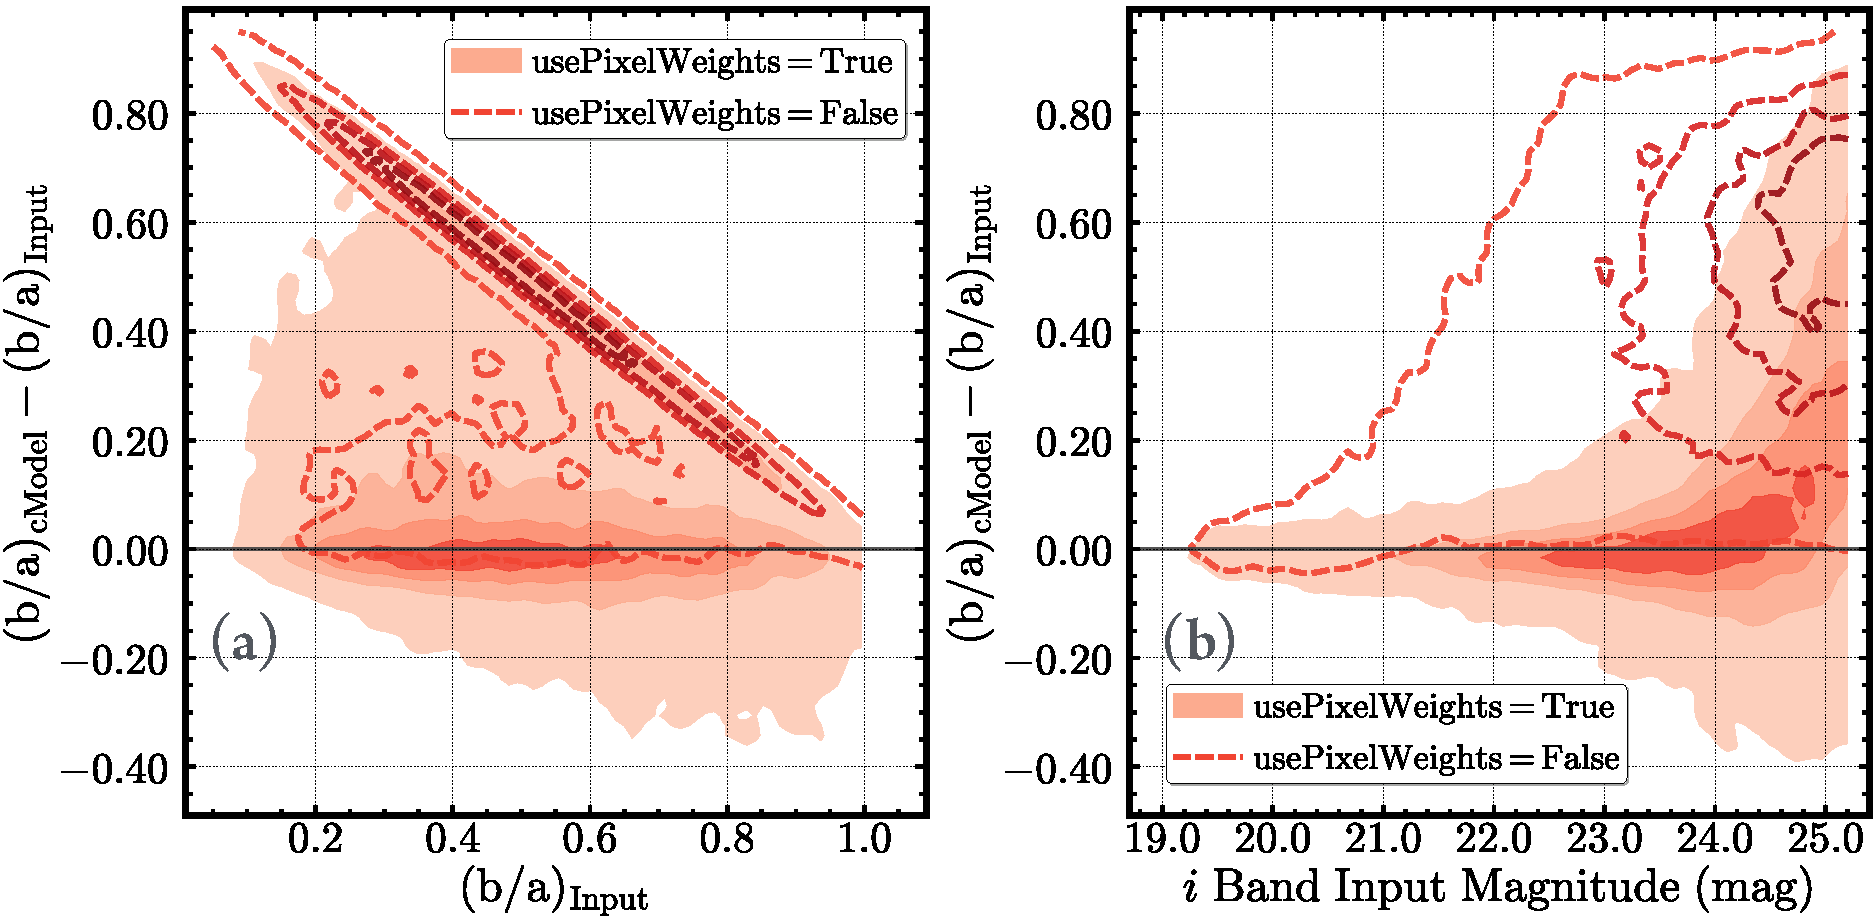
\includegraphics[width=\textwidth]{fig/synpipe_galaxy_ba}
    \end{center}
    \caption{
        Shows the accuracy of the weighted axis ratio measurements for synthetic
        galaxies using \cmodel{} photometry.
        \textbf{Left} shows the relation between the input $(b/a)$ and the
        uncertainties of $(b/a)$ estimates.
        \textbf{Right} shows the relation between input magnitude of synthetic galaxy
        and the $(b/a)$ uncertainties.
        Contours are for the default test with \texttt{usePixelWeights=False}, and the
        hexagonal bins are used for same tests with \texttt{usePixelWeights=True}.
        }
    \label{fig:galaxy_ba}
\end{figure*}
%% ------------------------------------------------------------------------------------ %%


%% ------------------------------------------------------------------------------------ %%

\section{Results on Other Aspects of \hscpipe{}}
    \label{sec:others}

    In this section, we briefly discuss a few other issues of \hscpipe{} that relates 
    to astrometric calibration, star-galaxy separation, and measurements of galaxy 
    shape to demonstrate the ranges of topics can be tested by \synpipe{}
    
%% ------------------------------------------------------------------------------------ %%
\subsection{Astrometric Calibration}
    \label{ssec:astrometry}
    
    For \synpipe{} test, we inject synthetic objects to single \visit{} images using 
    the less accurate, initial astrometric calibration. 
    During the image stacking step, the joint calibration process will improve the 
    astrometric solutions. 
    Therefore the differences between the input and output coordinates from \synpipe{}
    can help understand the systematic effect of this step. 
    
    In Fig \ref{fig:astrometry}, we plot the distributions of astrometric offsets for 
    both synthetic stars and galaxies in good- and bad-seeing \tracts{}. 
    Small systematic offsets at ${\sim}10$--20 mas can be noticed in either direction. 
    The two \tracts{} apparently show different systematic offsets. 
    In the same \tracts{}, synthetic stars and galaxies show very similar offsets, 
    although the scatter for galaxies is slightly larger due to their extended nature.
    
%% ------------------------------------------------------------------------------------ %%
\subsection{Star-Galaxy Separation}
    \label{ssec:sg}
    
    As we already mentioned, star--galaxy separation is important for cosmology survey,
    and becomes increasingly difficult for fainter and fainter objects. 

    \begin{itemize}

        \item \plan{Explain how star--galaxy separation is done in \hscpipe{}, and
            why it is difficult at faint magnitudes.}

        \item In Fig \ref{fig:sg}, we highlight the misclassified stars and galaxies
            on the relations between the input magnitude and
            $i_{\mathrm{PSF}}-i_{\mathrm{cModel}}$.

        \item \plan{The fraction of misclassified stars show dependence on both
            input magnitude and seeing.}

        \item \plan{Most of the misclassified galaxies have $i > 24.0$.
            The fraction of misclassification and distribution of
            $i_{\mathrm{PSF}}-i_{\mathrm{cModel}}$ for synthetic galaxies also depend on
            seeings}.

    \end{itemize}

%% ------------------------------------------------------------------------------------ %%
\subsection{Blendedness and Photometric Errors}
    \label{ssec:blendedness}

    \plan{Review the definition of blendedness and explain why it is important.}
    \plan{Relationship between magnitude and blendedness}

    \plan{How blendedness affects the photometric uncertainties}

%% ------------------------------------------------------------------------------------ %%
\subsection{Comparing to Kron photometry}

    \plan{Uses $i$-band as example to briefly discuss Kron photometry}

    \plan{Although magnitude for galaxies is Ok, the color becomes worse}

%% ------------------------------------------------------------------------------------ %%
\subsection{Shape and Structural Parameters of Galaxies}
    \label{ssec:shape}

    \plan{Explain why the current \cmodel{}{} algorithm has problem with measuring
          the size and shape of galaxies}

    \plan{Briefly showcase the problem, and how small change of \hscpipe{}
          configuration can improve the situation}
%% ------------------------------------------------------------------------------------ %%

%% ------------------------------------------------------------------------------------ %%
\section{Summary and Conclusion}
    \label{sec:summary}

    %% Short summary
    The on-going HSC survey just had its first public data release, and is still
    producing increasingly larger amount of high-quality imaging data.
    To help achieve the designed goals of the survey and facilitate scientific
    outputs, we develop \synpipe{}, a flexible framework that is based on the
    \hscpipe{} to exam the data reduction process and check the accuracy of all the
    pipeline outputs.
    \synpipe{} injects synthetic stars and galaxies to the desired locations on the
    single-\visit{} images with the help of the original astrometric and
    photometric calibrations.
    These data are then processed by \hscpipe{} to generate the coadd images and
    all the photometric measurements.
    In this way, \synpipe{} can simulate the realistic data reduction process
    to an extent that many subtle systematical effects can be taken into
    consideration, which is helpful for the outstanding scientific goals of the HSC
    survey.
    In this work, we choose two \tracts{} in the HSC/Wide layer with
    representative seeing conditions (good/bad) to test the general behaviors of HSC
    photometry for both stars and galaxies.

    From these tests, we find:

    \begin{enumerate}

        \item The \forced{} PSF photometry provides excellent magnitude and color
            measurements for isolated stars at $18.0 < i < 25.0$.
            The typical uncertainties of HSC forced PSF photometry for stars range
            from around 0.01 mag at $i{\sim}18.0$ mag to 0.08 mag at $i{\sim}25.0$
            mag (1\%-7\% accuracy in the $i$-band).
            The \forced{} PSF photometry can accurately recover the color--color
            sequences for stars.

        \item The \forced{} \cmodel{} photometry is reliable for synthetic galaxies
            with realistic distributions of structural parameters and colors at
            $20.0 < i < 25.0$ mag.
            The average accuracy of \forced{} \cmodel{} magnitude ranges from
            ${\sim}7$\% at $i{\sim}20.0$ mag to ${\sim}10$\% at $i{\sim}25.0$.
            The \forced{} \cmodel{} colors for galaxies are accurate and unbiased.
            The accuracies of colors do not show dependence on input magnitude and
            color.

        \item The \forced{} PSF and \cmodel{} photometry are robust against different
            seeing conditions, despite that worse seeing leads to lower
            $\mathrm{S}/\mathrm{N}$ at fixed input magnitude.

        \item High blendedness ($b>0.1$) impacts the accuracy of both PSF and \cmodel{}
            photometry, especially for stars.
            For highly blended stars, the \forced{} PSF photometry on average
            overestimate the magnitudes of stars by 0.1–-0.2 mag.
            For galaxies, high-blendedness typically adds an additional 0.05 mag
            uncertainty in both magnitude and color estimates.

    \end{enumerate}

    Meanwhile, we also notice a few issues in the current \hscpipe{}:

    \begin{enumerate}

        \item The performance of current star--galaxy separation algorithm in \hscpipe{}
            is not perfect, especially at faint magnitude end and under poor seeing
            condition.
            The fraction of stars that are misclassified as extended objects is still
            quite high ($>20$\% at $i> 22.5$ mag).

        \item The \cmodel{} setting right now (\texttt{usePixelWeights=True}) results
            in very biased estimates of shape and size for galaxies, especially for the
            relative faint ones.
            The axis ratio of galaxy using \cmodel{} is highly overestiamted while
            the effective radius is underestimated.
            We show that, using \texttt{usePixelWeights=True} instead and significantly
            improve this situation.
            However, it may impact the accuracy of deblender, which we will test in the
            future.

    \end{enumerate}

    The HSC collaboration is working on improving these issues in the future version
    of \hscpipe{} and the following data release.
    Meanwhile, we suggest the users of HSC data to keep these caveats in mind.
%% ------------------------------------------------------------------------------------ %%

%% ------------------------------------------------------------------------------------ %%
    %% Other applications
    Although we mainly focus on the general behaviors of photometric measurements here,
    \synpipe{} is quite flexible and has plenty of other applications for any HSC
    dataset.
    For instance, in a following paper, Murata\etal (in prep.) uses \synpipe{} to test
    the impacts of extremely blended objects on the WL measurements.
    Also, \citep{Niikura2017} applies \synpipe{} to the high-cadence HSC observations
    of M31 to help the search of interesting microlensing events.
    At this moment, it is also being used to estimate the completeness of the selections 
    for high-$z$ Lyman-break galaxies (LBG) and Lyman- $\alpha$ emitters 
    (Ono\etal in prep.; Konno\etal in prep), check the dependence of the detection and 
    completeness of high-$z$ LBG pairs on the pair separation (Harikane\etal in prep.),
    identify low surface brightness dwarf galaxies (Greco\etal in prep),
    and test photometric and WL measurements around nearby clusters (Chiu\etal in prep).

    %% Caveats
    In the end, it is worth brief discussing the limitations of the current \synpipe{}:

    \begin{enumerate}

        \item \citet{HSCDR1} points out that \hscpipe{} tends to over-subtract the
            background around bright objects.
            Unfortunately, \synpipe{} now takes the original background subtraction on
            the single-\visit{} image for granted, hence lacks the capability to
            test or help improve this problem.

        \item Right now, \synpipe{} simply adopts the PSF measured by \hscpipe{} and
            use it for model of point source and PSF convolution for galaxy.
            Hence it can not be used to test how the uncertainty of the PSF modeling
            affects the photometry and shape measurements.
            This could be important for regions with exquisite seeing that makes the
            PSF modeling difficult, and for accurate WL measurements.

        \item \synpipe{} now works in ``unit'' of \visit{} for single exposure
            test, and \tract{} for test of \texttt{coadd} images.
            In case of tests that focus on specific regions that are much smaller than
            the size of \visit{} or \tract{} (e.g. quality of photometry
            around rich galaxy clusters), the usage of \synpipe{} often leads to
            low efficiency.

    \end{enumerate}

    %% Future developments
    Right now, both \hscpipe{} and \synpipe{} still undergo active development,
    and \synpipe{} will update accordingly to provide photometric benchmark for
    each data release of HSC survey, and help \hscpipe{} improve.
    At the same time, we are also working on improving the efficiency of \synpipe{}.
    Since subtle effects involved in the image stacking process are not the concerns
    of many topics, we will update \synpipe{} so that it can directly inject
    synthetic objects to the coadd images and speed up these tests.

%% ------------------------------------------------------------------------------------ %%

%% ------------------------------------------------------------------------------------ %%

\begin{ack}
    \label{sec:ack}

    % HSC part
    The Hyper Suprime-Cam (HSC) collaboration includes the astronomical communities of
    Japan and Taiwan, and Princeton University.
    The HSC instrumentation and software were developed by the National Astronomical
    Observatory of Japan (NAOJ), the Kavli Institute for the Physics and Mathematics of
    the Universe (Kavli IPMU), the University of Tokyo, the High Energy Accelerator
    Research Organization (KEK), the Academia Sinica Institute for Astronomy and
    Astrophysics in Taiwan (ASIAA), and Princeton University.
    Funding was contributed by the FIRST program from Japanese Cabinet Office, the
    Ministry of Education, Culture, Sports, Science and Technology (MEXT), the Japan
    Society for the Promotion of Science (JSPS), Japan Science and Technology Agency
    (JST), the Toray Science  Foundation, NAOJ, Kavli IPMU, KEK, ASIAA, and Princeton
    University.

    % LSST software part
    This paper makes use of software developed for the Large Synoptic Survey Telescope.
    We thank the LSST Project for making their code available as free software at
    http://dm.lsstcorp.org.

    % Pan-STARRS1 part
    The Pan-STARRS1 Surveys (PS1) have been made possible through contributions of the
    Institute for Astronomy, the University of Hawaii, the Pan-STARRS Project Office,
    the Max-Planck Society and its participating institutes, the Max Planck Institute
    for Astronomy, Heidelberg and the Max Planck Institute for Extraterrestrial Physics,
    Garching, The Johns Hopkins University, Durham University, the University of
    Edinburgh, Queen's University Belfast, the Harvard-Smithsonian Center for Astrophysics,
    the Las Cumbres Observatory Global Telescope Network Incorporated, the National
    Central University of Taiwan, the Space Telescope Science Institute, the National
    Aeronautics and Space Administration under Grant No.
    NNX08AR22G issued through the Planetary Science Division of the NASA Science
    Mission Directorate, the National Science Foundation under Grant No. AST-1238877,
    the University of Maryland, and Eotvos Lorand University (ELTE) and the Los Alamos
    National Laboratory.

    % Software part
    This research made use of
    {\texttt{Astropy}},
        a community-developed core Python package for Astronomy (\citealt{Astropy};
        \url{http://www.astropy.org/});
    {\texttt{astroML}},
        a machine learning library for astrophysics (\citealt{astroml};
        \url{http://www.astroml.org/});
    {\texttt{SciPy}},
        an open source scientific tools for Python (\citealt{SciPy};
        \url{http://www.scipy.org/});
    {\texttt{NumPy}},
        a fundamental package for scientific computing with Python (\citealt{NumPy};
        \url{http://www.numpy.org/});
    {\texttt{Matplotlib}},
        a 2-D plotting library for Python (\citealt{Matplotlib};
        \url{http://matplotlib.org/});
    {\texttt{scikit-learn}},
        a machine-learning library in Python (\citealt{scikit-learn};
        \url{http://scikit_learn.org/}).

\end{ack}
%% ------------------------------------------------------------------------------------ %%

%%%%%%%%%%: Bibliographic Section %%%%%%%%%%

%\bibliography{synpipe}

%% ------------------------------------------------------------------------------------ %%
\bibliographystyle{apj}

%% ------------------------------------------------------------------------------------ %%
\begin{thebibliography}{}
    \label{sec:ref}
    \expandafter\ifx\csname natexlab\endcsname\relax\def\natexlab#1{#1}\fi

    %% A %%
    \bibitem[Abazajian et al.(2004)]{Abazajian2004} Abazajian, K., Adelman-McCarthy,
             J.~K., Ag{\"u}eros, M.~A., et al.\ 2004, \aj, 128, 502

    \bibitem[Aihara et al.(2017)]{HSCDR1} Aihara, H., Armstrong, R., Bickerton, S.,
             et al.\ 2017, arXiv:1702.08449

    \bibitem[Antilogus et al.(2014)]{2014JInst...9C3048A} Antilogus, P., Astier, P.,
             Doherty, P., Guyonnet, A., \& Regnault, N.\ 2014, Journal of
             Instrumentation, 9, C03048

    \bibitem[Astropy Collaboration et al.(2013)]{Astropy} Astropy Collaboration,
             Robitaille, T.~P., Tollerud, E.~J., et al.\ 2013, \aap, 558, A33

    \bibitem[Axelrod et al.(2010)]{Axelrod2010} Axelrod, T., Kantor, J., Lupton,
             R.~H., \& Pierfederici, F.\ 2010, \procspie, 7740, 774015

    %% B %%
    \bibitem[Bartelmann \& Schneider(2001)]{Bartelmann2001} Bartelmann, M., \&
             Schneider, P.\ 2001, \physrep, 340, 291

    \bibitem[Ben{\'{\i}}tez(2000)]{Benitez2000} Ben{\'{\i}}tez, N.\ 2000, \apj,
             536, 571

    \bibitem[Bertin(2011)]{Bertin2011} Bertin, E.\ 2011, Astronomical Data Analysis
             Software and Systems XX, 442, 435

    \bibitem[Bertin(2013)]{Bertin2013} Bertin, E.\ 2013, Astrophysics Source
             Code Library, ascl:1301.001

    \bibitem[Bolzonella et al.(2000)]{Bolzonella2000} Bolzonella, M., Miralles, J.-M.,
            \& Pell{\'o}, R.\ 2000, \aap, 363, 476

    \bibitem[Bovy Jo et al.(2011)]{Bovy2011} Bovy Jo, Hogg, D.~W., \& Roweis,
             S.~T.\ 2011, Annals of Applied Statistics, 5,

    %% C %%
    \bibitem[Chang et al.(2015)]{Chang2015} Chang, C., Busha, M.~T., Wechsler, R.~H.,
             et al.\ 2015, \apj, 801, 73

    %% D %%
    \bibitem[Dressler et al.(2012)]{Dressler2012} Dressler, A., Spergel, D., Mountain,
             M., et al.\ 2012, arXiv:1210.7809

    %% G %%
    \bibitem[Greisen \& Calabretta(2002a)]{WCS1} Greisen, E.~W., \& Calabretta, M.~R.\
             2002, \aap, 395, 1061

    \bibitem[Calabretta \& Greisen(2002b)]{WCS2} Calabretta, M.~R., \& Greisen, E.~W.\
             2002, \aap, 395, 1077

    %% H %%
    \bibitem[Hunter (2007)]{Matplotlib} Hunter J. D., 2007, Computing In Science \&
             Engineering, 9, 90

    %% I %%
    \bibitem[Ilbert et al.(2009)]{Ilbert2009} Ilbert, O., Capak, P., Salvato,
             M., et al.\ 2009, \apj, 690, 1236

    \bibitem[Ivezic et al.(2008)]{Ivezic2008} Ivezic, Z., Axelrod, T., Brandt, W.~N.,
             et al.\ 2008, Serbian Astronomical Journal, 176, 1

    %% J %%
    \bibitem[Jones et al.(2001)]{SciPy} Jones E., Oliphant T., Peterson P., et al.,
             2001, SciPy: Open source scientific tools for Python,
             \url{http://www.scipy.org/}

    \bibitem[Juri{\'c} et al.(2015)]{Juric2015} Juri{\'c}, M., Kantor, J., Lim, K.,
             et al.\ 2015, arXiv:1512.07914

    %% K %%
    \bibitem[Kaiser \& Squires(1993)]{Kaiser1993} Kaiser, N., \& Squires, G.\
             1993, \apj, 404, 441

    %% L %%
    \bibitem[Lackner \& Gunn(2012)]{Lackner2012} Lackner, C.~N., \& Gunn, J.~E.\
             2012, \mnras, 421, 2277

    \bibitem[Laureijs et al.(2012)]{Laureijs2012} Laureijs, R., Gondoin, P., Duvet, L.,
             et al.\ 2012, \procspie, 8442, 84420T

    \bibitem[Leauthaud et al.(2007)]{Leauthaud2007} Leauthaud, A., Massey, R.,
             Kneib, J.-P., et al.\ 2007, \apjs, 172, 219

    \bibitem[Lupton et al.(2001)]{Lupton2001} Lupton, R., Gunn, J.~E., Ivezi{\'c},
             Z., Knapp, G.~R., \& Kent, S.\ 2001, Astronomical Data Analysis Software
             and Systems X, 238, 269

    %% M %%
    \bibitem[Magnier et al.(2013)]{Magnier2013} Magnier, E.~A., Schlafly, E.,
             Finkbeiner, D., et al.\ 2013, \apjs, 205, 20

    \bibitem[Mandelbaum et al.(2014)]{Mandelbaum2014} Mandelbaum, R., Rowe, B.,
            Bosch, J., et al.\ 2014, \apjs, 212, 5

    \bibitem[Mandelbaum et al.(2015)]{Mandelbaum2015} Mandelbaum, R., Rowe, B.,
             Armstrong, R., et al.\ 2015, \mnras, 450, 2963

    \bibitem[Miyazaki et al.(2012)]{Miyazaki2012} Miyazaki, S., Komiyama, Y., Nakaya,
             H., et al.\ 2012, \procspie, 8446, 84460Z

    %% N %%
    \bibitem[Niikura et al.(2017)]{Niikura2017} Niikura, H., Takada, M., Yasuda, N.,
             et al.\ 2017, arXiv:1701.02151

    %% P %%
    \bibitem[Padmanabhan et al.(2008)]{Padmanabhan2008} Padmanabhan, N., Schlegel,
             D.~J., Finkbeiner, D.~P., et al.\ 2008, \apj, 674, 1217-1233

    \bibitem[Pedregosa et al.(2011)]{scikit-learn} Pedregosa F., et al., 2011,
             Journal of Machine Learning Research, 12, 2825

    %% R %%
    \bibitem[Rowe et al.(2015)]{Rowe2015} Rowe, B.~T.~P., Jarvis, M., Mandelbaum, R.,
             et al.\ 2015, Astronomy and Computing, 10, 121

    %% S %%
    \bibitem[Schlafly et al.(2012)]{Schlafly2012} Schlafly, E.~F., Finkbeiner, D.~P.,
             Juri{\'c}, M., et al.\ 2012, \apj, 756, 158

    \bibitem[Scoville et al.(2007)]{Scoville2007} Scoville, N., Abraham, R.~G.,
             Aussel, H., et al.\ 2007, \apjs, 172, 38

    \bibitem[S{\'e}rsic(1963)]{Sersic1963} S{\'e}rsic, J.~L.\ 1963, Boletin de la
             Asociacion Argentina de Astronomia La Plata Argentina, 6, 41

    \bibitem[Suchyta et al.(2016)]{Suchyta2016} Suchyta, E., Huff, E.~M., Aleksi{\'c},
             J., et al.\ 2016, \mnras, 457, 786

    \bibitem[Steidel et al.(1996)]{Steidel1996} Steidel, C.~C., Giavalisco, M.,
             Pettini, M., Dickinson, M., \& Adelberger, K.~L.\ 1996, \apjl, 462, L17

    %% T %%
    \bibitem[The Dark Energy Survey Collaboration(2005)]{DES2005} The Dark Energy
             Survey Collaboration 2005, arXiv:astro-ph/0510346

    \bibitem[Tonry et al.(2012)]{Tonry2012} Tonry, J.~L., Stubbs, C.~W., Lykke, K.~R.,
             et al.\ 2012, \apj, 750, 99

    %% V %%
    \bibitem[VanderPlas et al.(2014)]{astroml} VanderPlas, J., Fouesneau, M., \&
             Taylor, J.\ 2014, Astrophysics Source Code Library, ascl:1407.018

    %% W %%
    \bibitem[Walt et al.(2011)]{NumPy} Walt S. v. d., Colbert S. C., Varoquaux G.,
             2011, Computing in Science and Engg., 13, 22

\end{thebibliography}
%% ------------------------------------------------------------------------------------ %%


%% ------------------------------------------------------------------------------------ %%
\appendix
%% ------------------------------------------------------------------------------------ %%
\section{Quality Control of Synthetic Objects}
    \label{app:qc}

    To select synthetic stars and galaxies from the results to test the photometry,
    we apply some basic quality control cuts here.

    The HSC survey defines the full--depth \& full--color regions (\texttt{FDFC}) to
    make sure the data used for science reach the expected number of exposures in each
    band
    ($\mathtt{(\#gri\ \geq\ 4)\ and\ (\#yz\ \geq\ 6)\ and\ (Limiting\ imag> 25.6)}$).
    And, the two \tracts{} we used in this work are almost entirely covered in
    the \texttt{FDFC} region so we do not apply this cut.
    We apply the following cuts to the matched synthetic objects"

    \begin{itemize}

        \item[ ] \texttt{ idetect\_is\_primary==True }
        \item[ ] \texttt{ ideblend\_skipped==False }
        \item[ ] \texttt{ iflags\_badcentroid==False }
        \item[ ] \texttt{ icentroid\_sdss\_flags==False }
        \item[ ] \texttt{ iflags\_pixel\_edge==False }
        \item[ ] \texttt{ iflags\_pixel\_interpolated\_center==False }
        \item[ ] \texttt{ iflags\_pixel\_saturated\_center==False }
        \item[ ] \texttt{ iflags\_pixel\_cr\_center==False }
        \item[ ] \texttt{ iflags\_pixel\_bad==False }
        \item[ ] \texttt{ iflags\_pixel\_suspect\_center==False }
        \item[ ] \texttt{ iflags\_pixel\_clipped\_any==False }
        \item[ ] \texttt{ iflags\_pixel\_bright\_object\_center ==False }

    \end{itemize}

    \todo{Details for stars and galaxies}

%% ------------------------------------------------------------------------------------ %%

%% ------------------------------------------------------------------------------------ %%
\section{$b$: The Blendedness Parameter}
    \label{app:defineb}

    To evaluate at what degree an object is blended with others, \hscpipe{} introduces
    the blendedness parameter: $b$ (\texttt{[grizy]blendedness\_abs\_flux}).
    Please refer to Bosch\etal (in prep.) and Murata\etal (in prep.) for more details,
    here we briefly explain the definition.

    For object ${\rm A}$:
    \begin{eqnarray*}
        b({\rm A}) \equiv
        1-\frac{\int_{\mathbb{R}^2} {\rm d}x~ {\rm d}y\ \mathcal{N}_{\mathrm{A}}({\bf x}\ |\  \mu_{\mathrm{A}}, {\bf\Sigma}_{\mathrm{A}})
        F_{\mathrm{A}}({\bf x})}{\int_{\mathbb{R}^2} {\rm d}x~ {\rm d}y\ \mathcal{N}_{\mathrm{A}}({\bf x}\ |\  \mu_{\mathrm{A}},
        {\bf\Sigma}_{\rm{A}}) F_{\rm{total}}({\bf x})},
        \label{eq:defineb}
    \end{eqnarray*}

    \noindent
    where $\mathcal{N}_{\rm{A}}({ \bf x }\ |\  \mu_{\rm{A}}, {\bf\Sigma}_{\rm{A}})$
    is a 2-D Gaussian function at pixel position $\bf x$, $\mu_{\mathrm{A}}$ is the
    estimated centroid of object ${\rm A}$, and covariance ${\bf \Sigma}_{\mathrm{A}}$
    is estimated based on the Gaussian-weighted adaptive second moments of object
    ${\rm A}$ (no PSF correction).
    $F_{\mathrm{total}}({\bf x })$ and $F_{\rm{A}}({\bf x })$ are pixels values of
    ${\rm A}$ before and after \hscpipe{} deblending process.

    By definition, the parameter is bound from 0 to 1.
    When the deblending process is carried out correctly, the $b({\rm A})$ parameter
    reflects the fraction of fluxes that comes from other objects in the
    region of ${\rm A}$.
%% ------------------------------------------------------------------------------------ %%

%% ------------------------------------------------------------------------------------ %%
%%%%%%%%%%%: Possible Tables %%%%%%%%%%%%%
%\input{table1.tex}
%% ------------------------------------------------------------------------------------ %%

%% ------------------------------------------------------------------------------------ %%
\label{lastpage}
\end{document}
%% ------------------------------------------------------------------------------------ %%
